\chapter{Adversarial Studies on DeepJet}

To evaluate the performance of adversarial attacks, the models nominal performance is assessed as a baseline for unperturbed input data. Based on this data, the input similarity (see \ref{sec:input_similarity}) is addressed for multi-iterational attacks of PGD, PIP and PIP-PGD. Furthermore, a PGD attack is applied as a reference for a successful attack. The JSD value is used throughout this entire chapter to quantify the mismatching of the given adversarial input. ROC Curves act as labels for the success of the attacks while being complemented by additional loss/validation curves that offer a broader view of the attacks performance. All attacks are evaluated in terms of attack severity, performance on nominal data, and adversarial-trained performance, followed by an analysis of their transferability and cross-robustness to determine whether PIP — alone or in combination with continuous-domain attacks — offers robustness beyond existing methods.

\section{Reference study}

This section establishes critical benchmarks for evaluating adversarial attacks on DeepJet. It first assesses the model's nominal performance under standard conditions to provide a baseline for unperturbed data. Then, it examines the impact of PGD attacks to set a reference for comparing subsequent adversarial strategies.

\subsection{Nominal Performance}

At nominal training and testing, the training validation yields a stable curve with a convergence at around 0.93. The validation is sitting slightly below at roughly 0.90 offering stable convergence too (see figure \ref{fig:nominal_training}). Figure \ref{fig:nominal_roc} portrays the identification score for BvsL found to be $AUC=0.965$.

\begin{figure}[htbp]
  \centering
  \begin{subfigure}[t]{0.59\textwidth}
    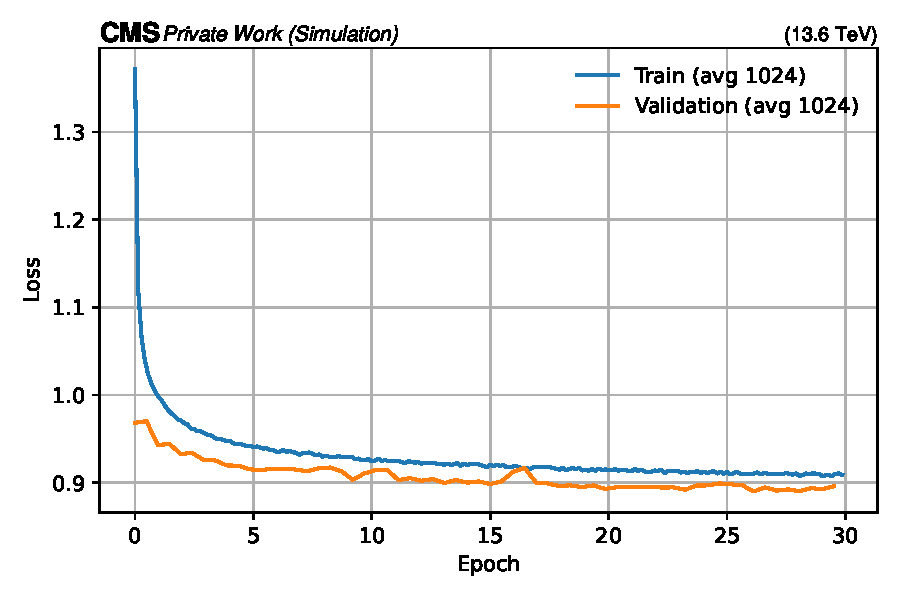
\includegraphics[width=\linewidth]{media/output/nominal_loss_validation.pdf}
    \caption{Training and validation loss for nominal training up to 30 epochs.}
    \label{fig:nominal_training}
  \end{subfigure}\hfill
  \begin{subfigure}[t]{0.41\textwidth}
    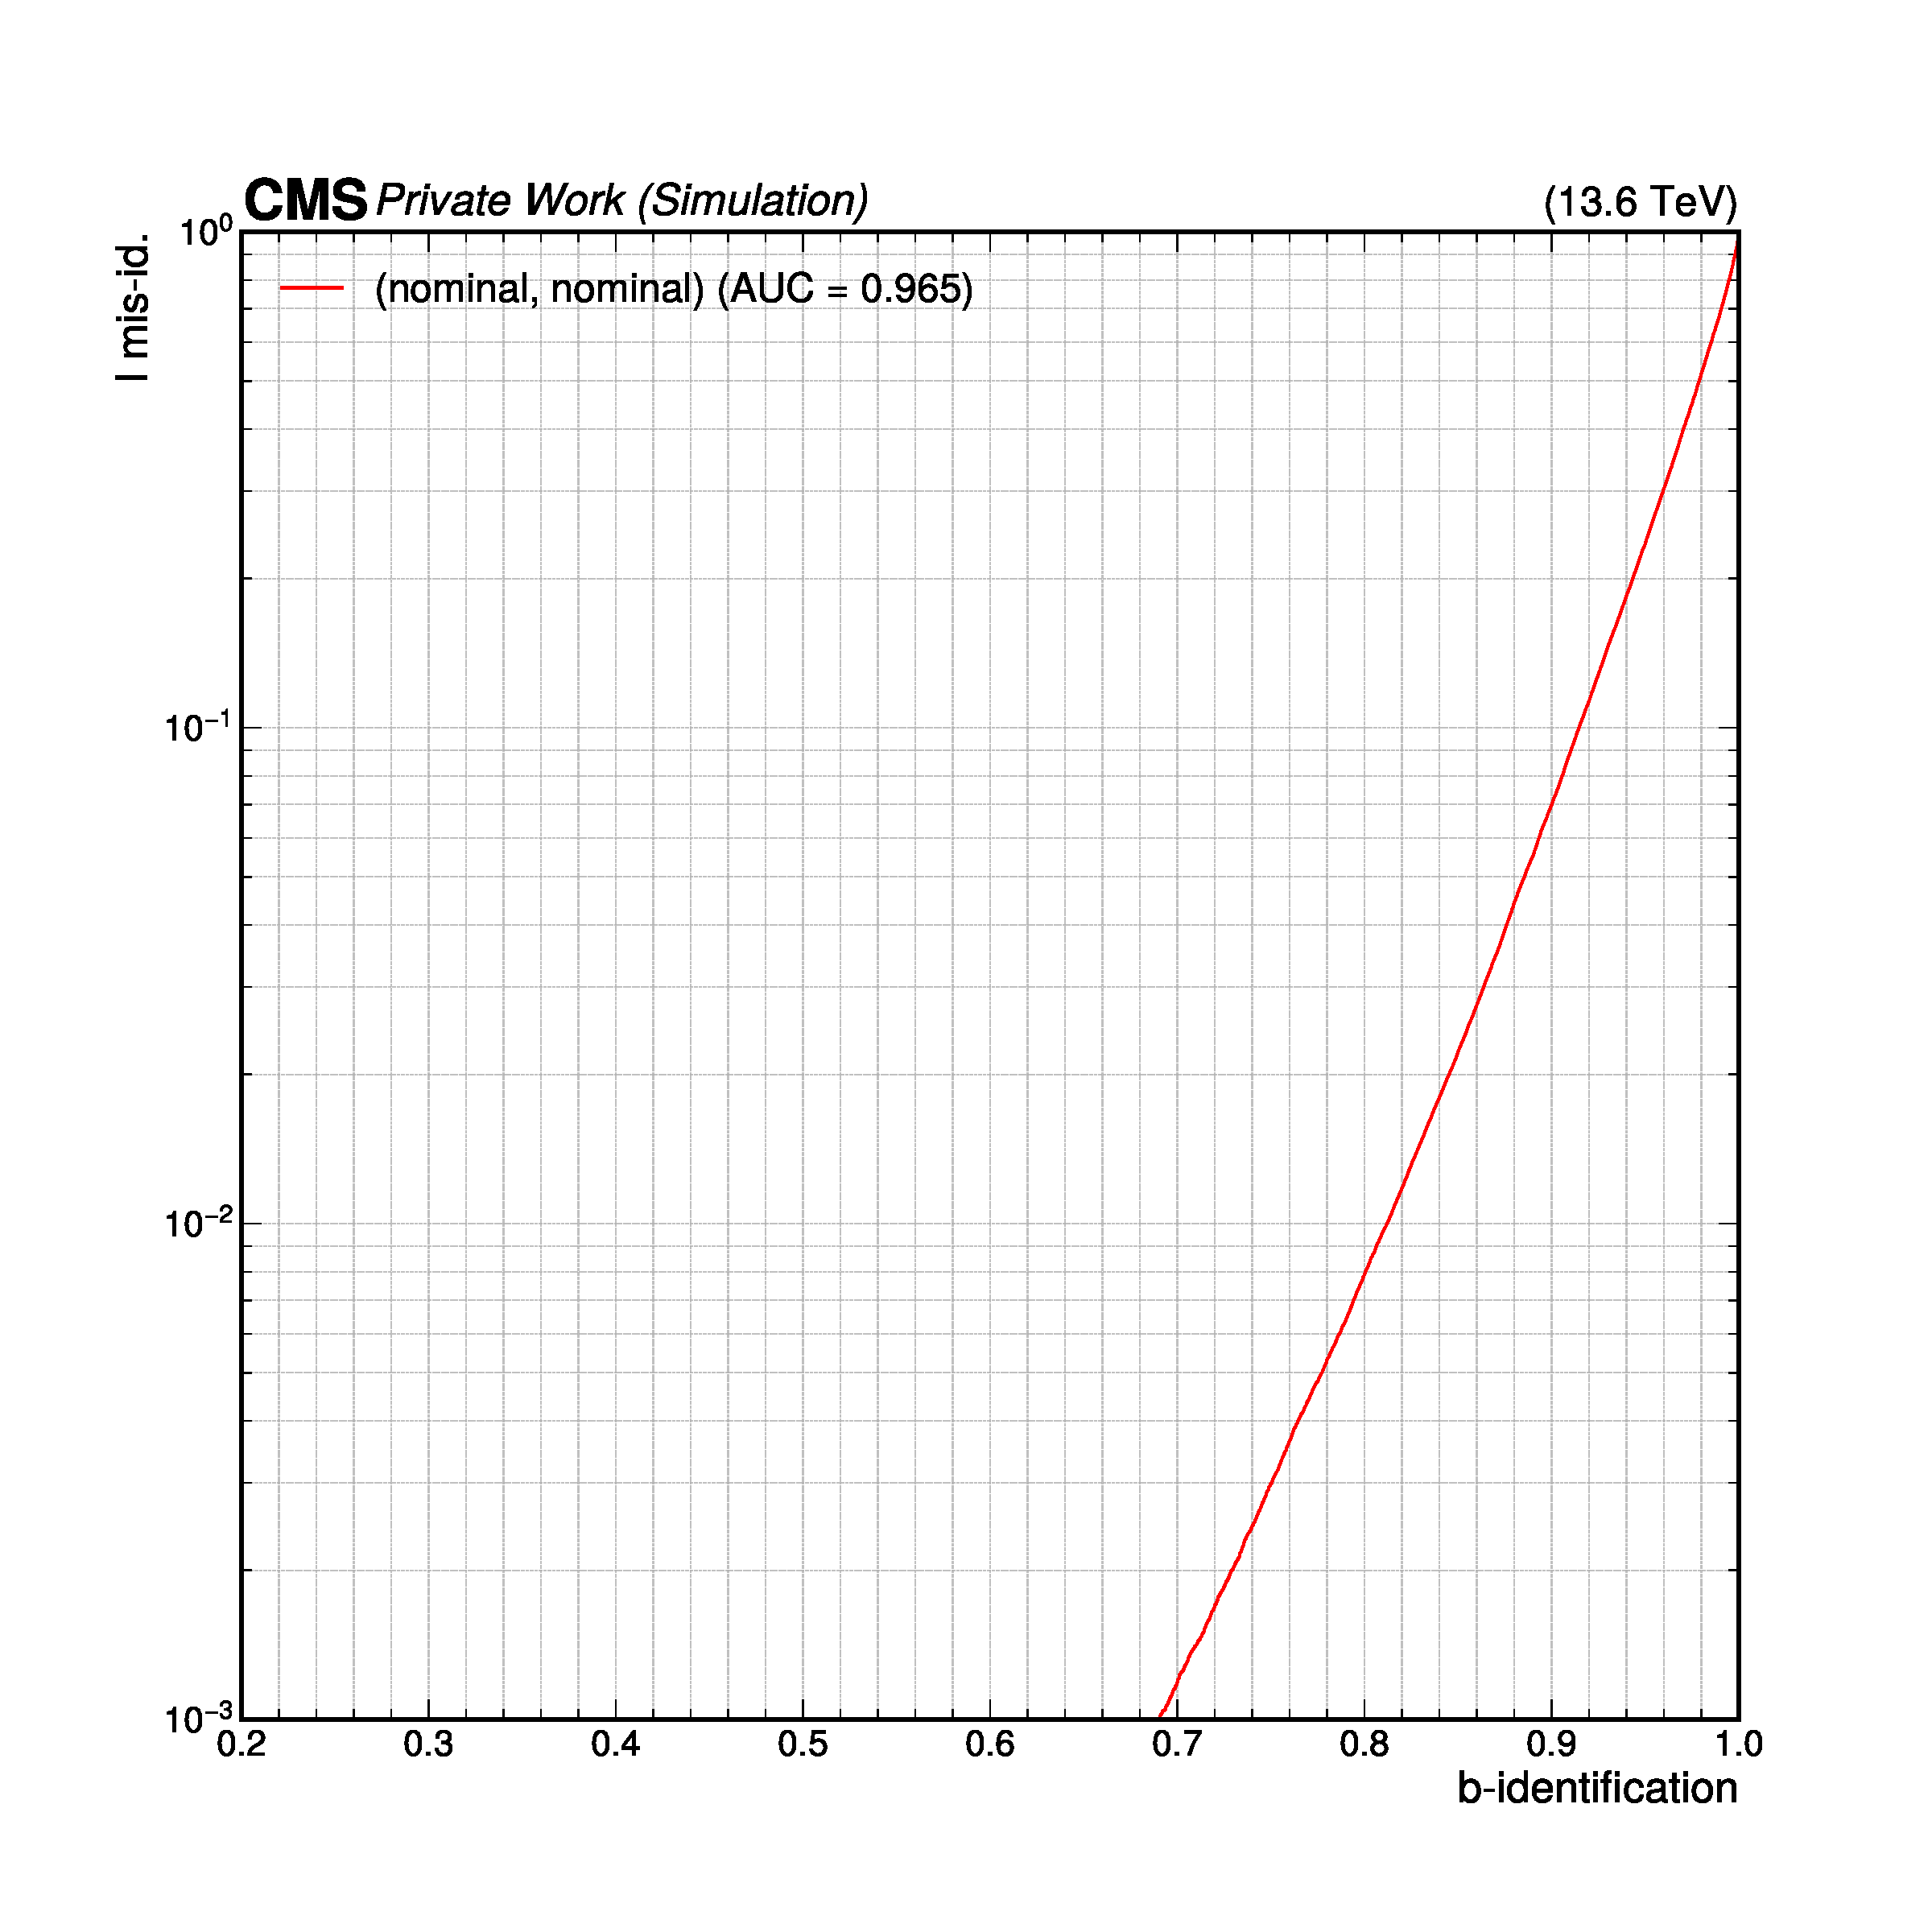
\includegraphics[width=\linewidth]{media/output/roc_bvsl_nominal_nominal.pdf}
    \caption{ROC Curve for the nominal trained baseline tested against nominal input.}
    \label{fig:nominal_roc}
  \end{subfigure}\hfill
\end{figure}

\FloatBarrier
\subsection{Projected Gradient Descent}

To assess the efficacy of the novel approach it is also necessary to look at well established adversarial attacks as an adversarial baseline — in this case PGD. For the sake of simplicity a magnitude of $\epsilon=0.1$ is applied for all following PGD attacks\footnote{As briefly discussed in section \ref{sec:fgsm_methodology} an additional scaling is applied proportional to the relative feature scale tensor $\varepsilon_{i,i}$. The behaviour for varying PGD magnitudes does not fall into the scope of this thesis.}.

\paragraph{Severity:} Figure \ref{fig:pgd_input_overview} provides a comprehensive view of input similarity across the entire input domain for up to three PGD iterations. The figure reveals an important patterns: 
(1) The JSD values for all features and iterations fall within the range of $\mathcal{O}(10^{-2})$ to $\mathcal{O}(10^{-3})$, in agreement to the threshold typically considered for stealthy attacks.
(2) The perturbation magnitude generally stays constant over multiple iteration. However, this is not uniform across all features; some features show minimal change even after multiple iterations, while others exhibit significant perturbation from the first iteration.

This selective perturbation behaviour stems from the gradient reassessment process inherent in PGD. Unlike single-step methods like FGSM that always assume the worst-case perturbation direction, PGD's iterative approach allows for more nuanced optimization. Features with strong gradients in the initial iterations may see their gradients diminish or even reverse direction in subsequent iterations, causing them to "project back" toward their original values. The overall perturbation pattern suggests that PGD attacks are highly targeted. They focus computational effort on features that provide the most leverage for compromising the classifier's performance.

\begin{figure}[H]
\centering
    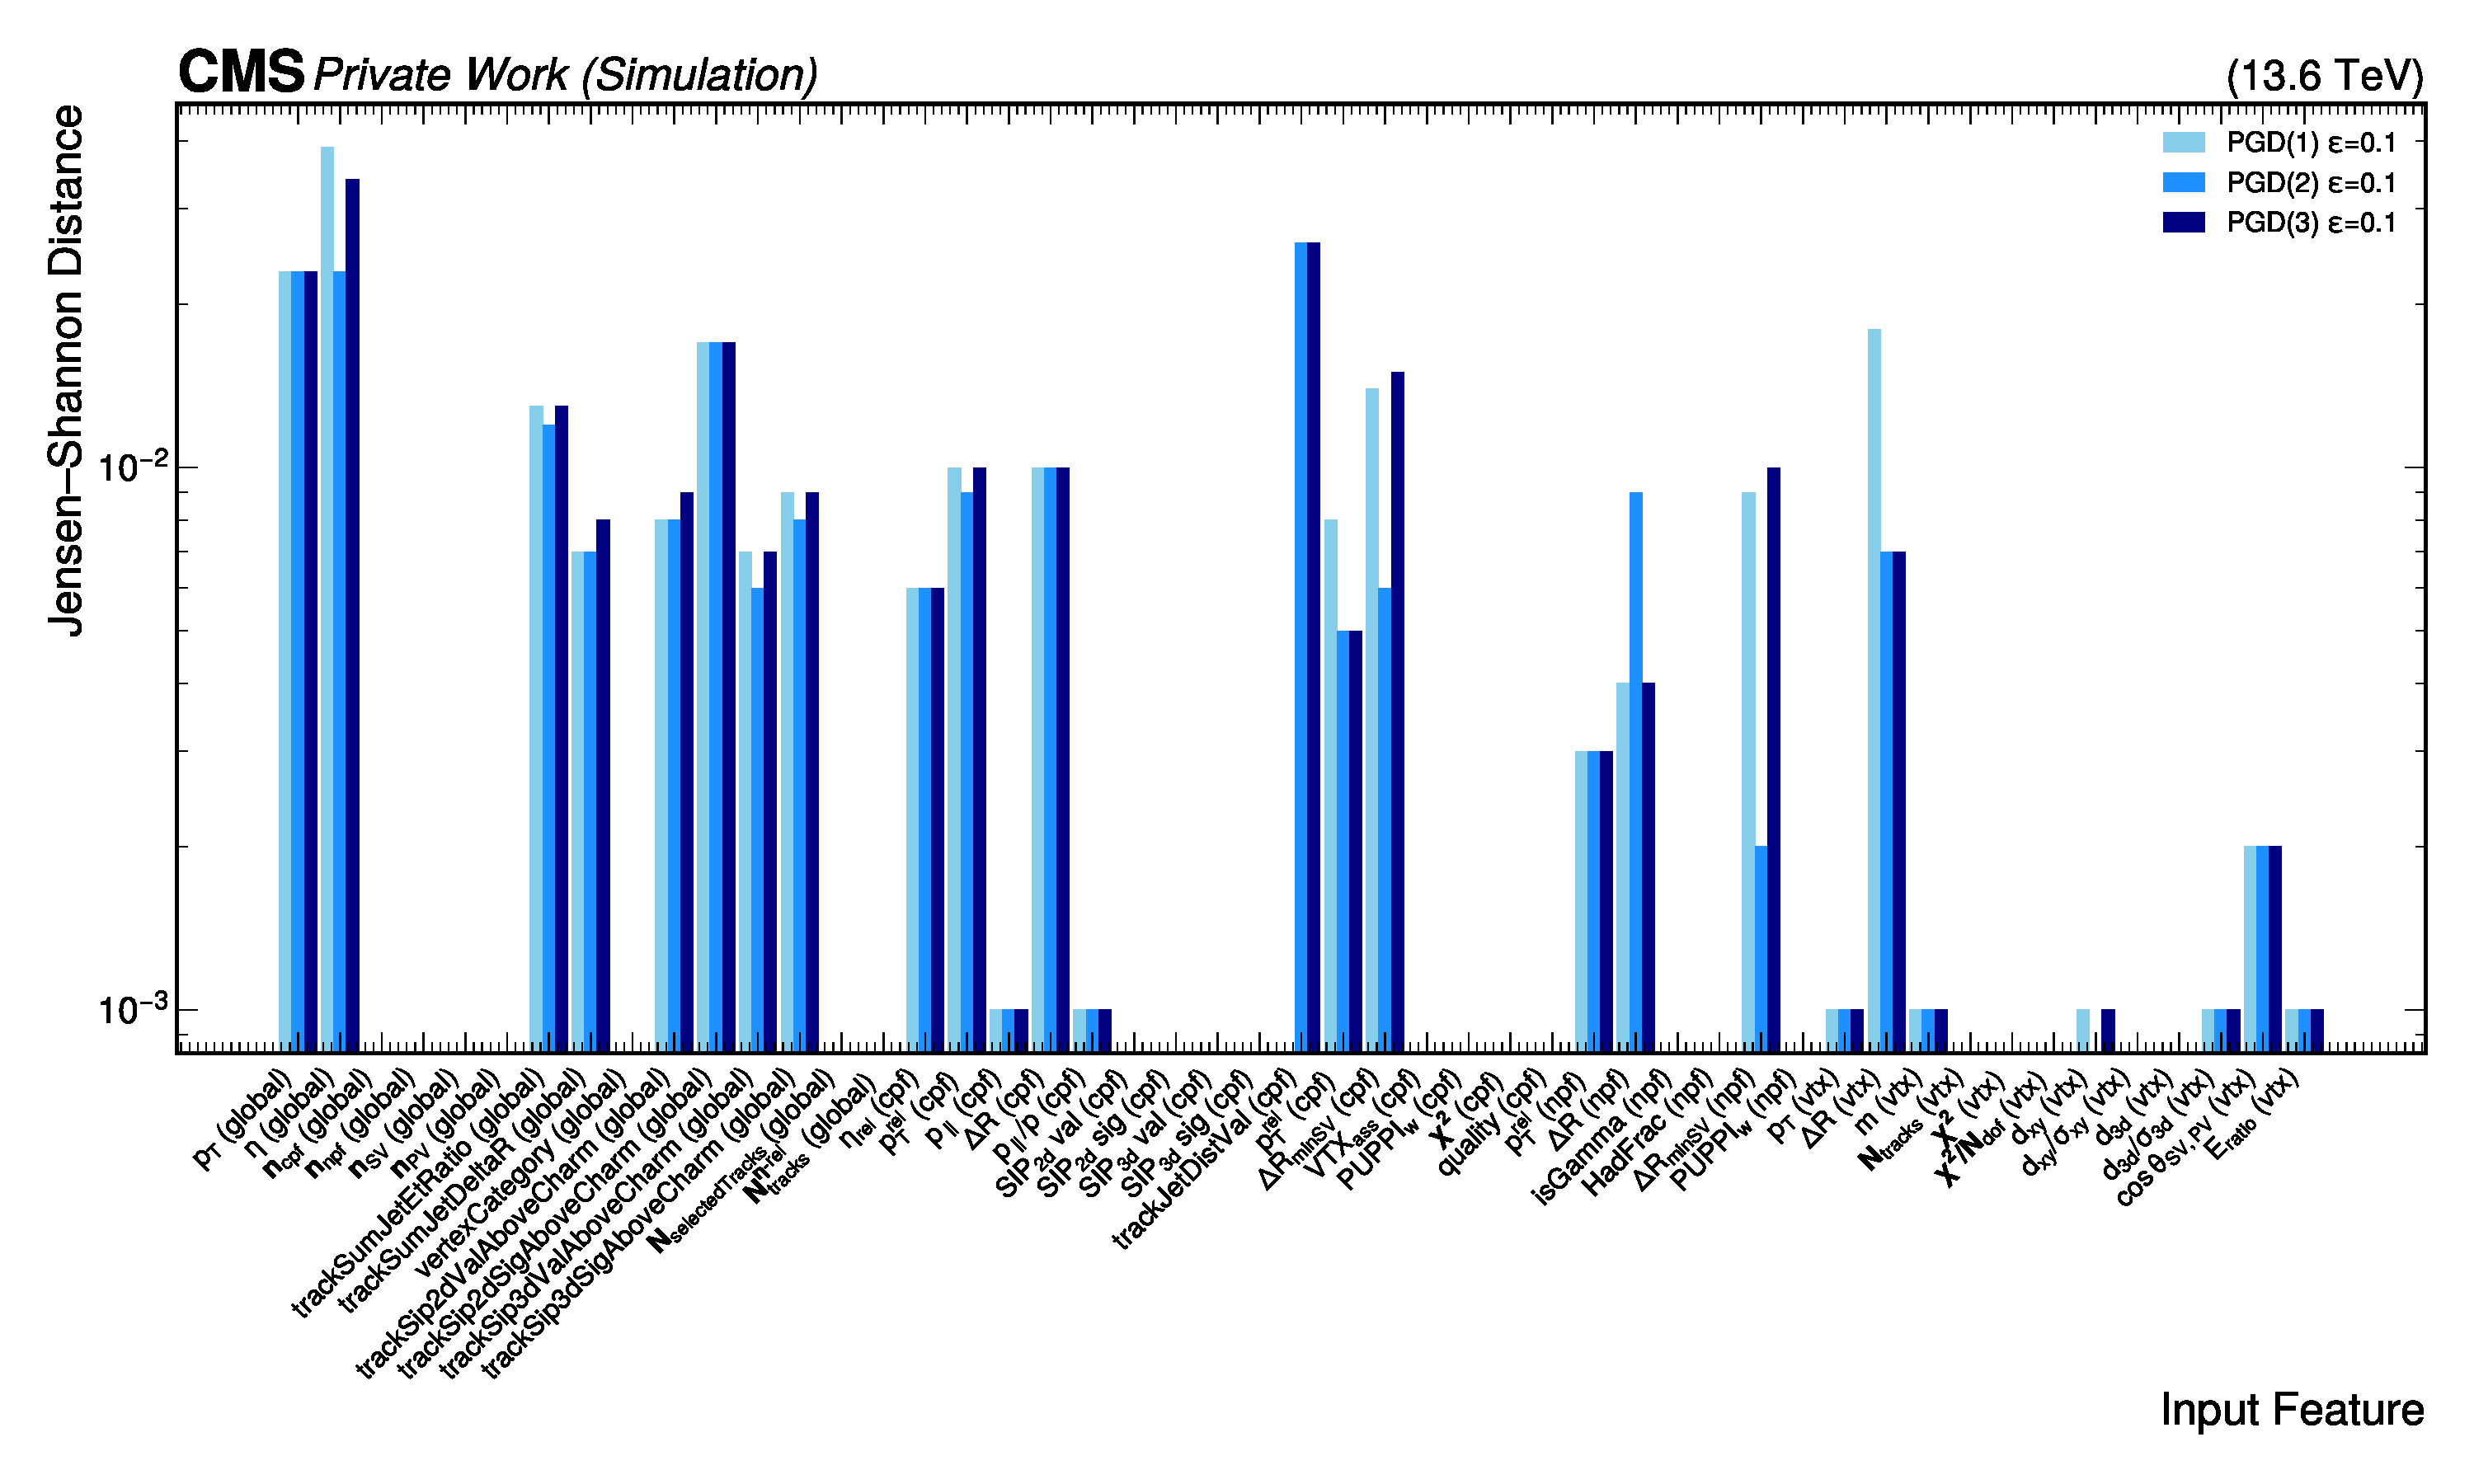
\includegraphics[width=15cm]{media/output/features/compare/jsd_pgd_iterations_featurewise_hor.pdf}
    \caption{JSD input similarity development for up to three iterations of the PGD attack with $\epsilon=0.1$ tested against a nominal trained model.}
    \label{fig:pgd_input_overview}
\end{figure}
\FloatBarrier
\newpage
\paragraph{Attack:} Figure \ref{fig:pgd_iterations} illustrates the impact of multiple PGD iterations on the BvsL discrimination task. The baseline nominal performance (AUC = 0.965) serves as the reference point against which attack efficacy is measured. The single-iteration PGD(1) attack achieves an AUC of approximately $0.937$, representing a clear reduction in performance. This initial attack demonstrates that even minimal adversarial perturbation can compromise the classifier's discriminative power. The two-iteration PGD(2) attack yields the same AUC score as PGD(1), while the three-iteration variant  reduces the AUC slightly to approximately 0.936.

This progressive degradation highlights two important aspects of PGD attacks. The iterative nature allows for more sophisticated perturbation strategies that can exploit the model's decision boundaries more effectively than single-step methods. Moreover, the diminishing returns observed between iterations 2 and 3 suggest that the attack approaches a performance floor, beyond which additional iterations provide minimal benefit.

\begin{figure}[h]
\centering
    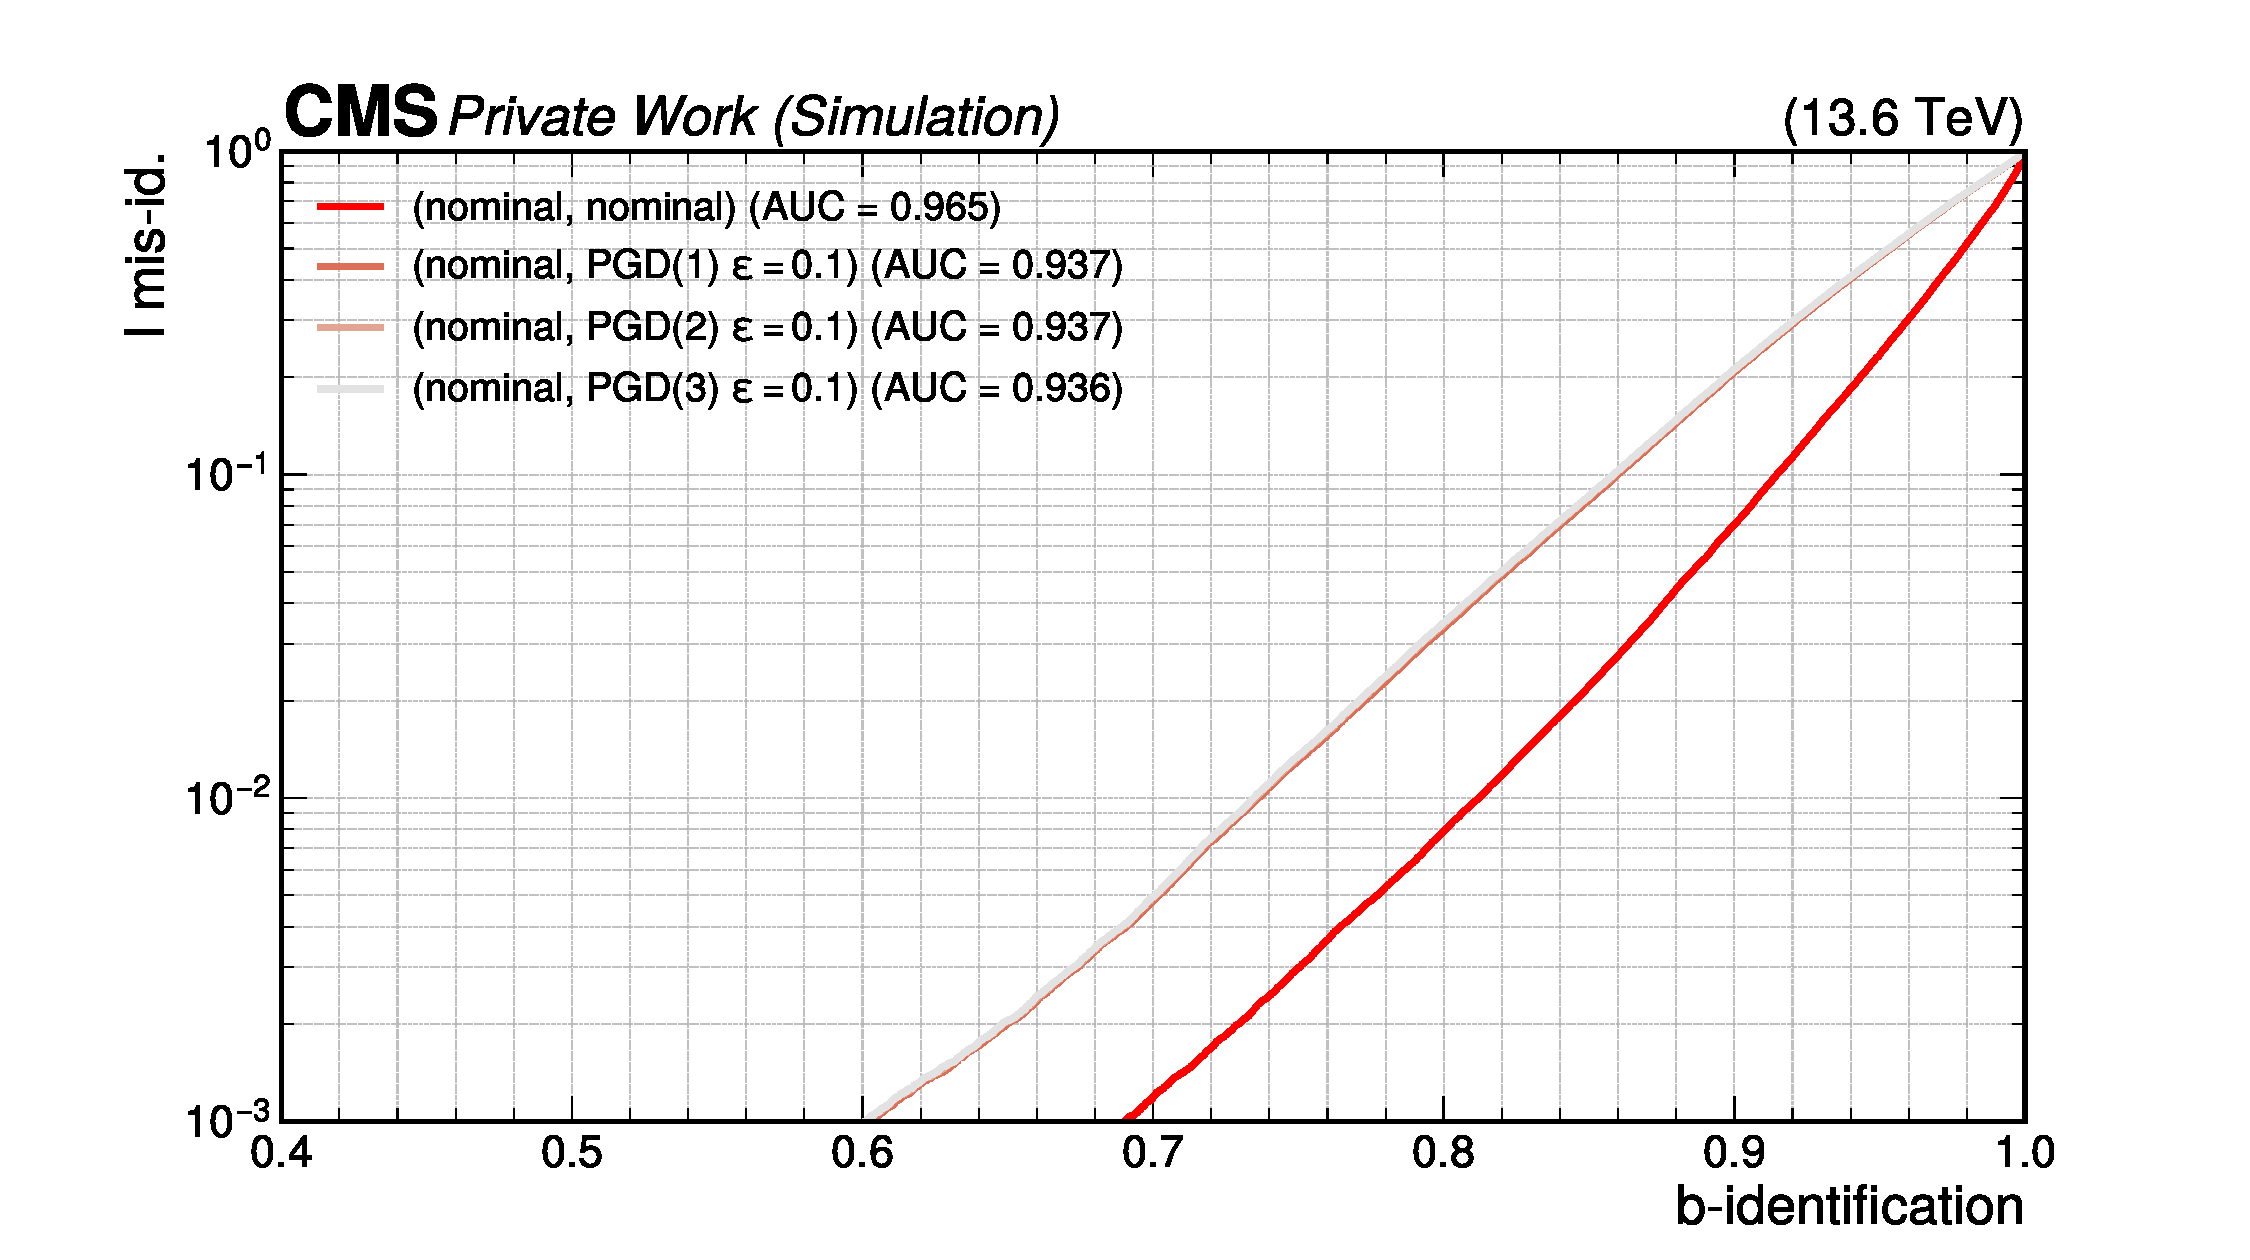
\includegraphics[width=15cm]{media/output/roc_bvsl_pgd_its_1_2_3.pdf}
    \caption{ROC curves for BvsL misidentification. Nominal trained model tested against one, two, and three iterations of PGD attacked inputs with $\epsilon=0.1$.}
    \label{fig:pgd_iterations}
\end{figure}

\paragraph{Adversarial Training:} Adversarial training with PGD perturbations introduces unique challenges to the learning process. The training and loss curve ( figure \ref{fig:pgd_loss_curve}) exhibit a higher spread between the convergence in loss (training sitting at approximately 1.0, validation at roughly 0.95), reflecting the inherent difficulty of learning robust representations under continuous adversarial perturbation. This is caused due to the necessity to simultaneously optimize for performance on clean data while developing defences against gradient-based attacks.

Notably, the training process achieves stable convergence despite the adversarial component. This means that PGD-based adversarial training is a viable strategy for improving model robustness.

\begin{figure}[h]
\centering
    
    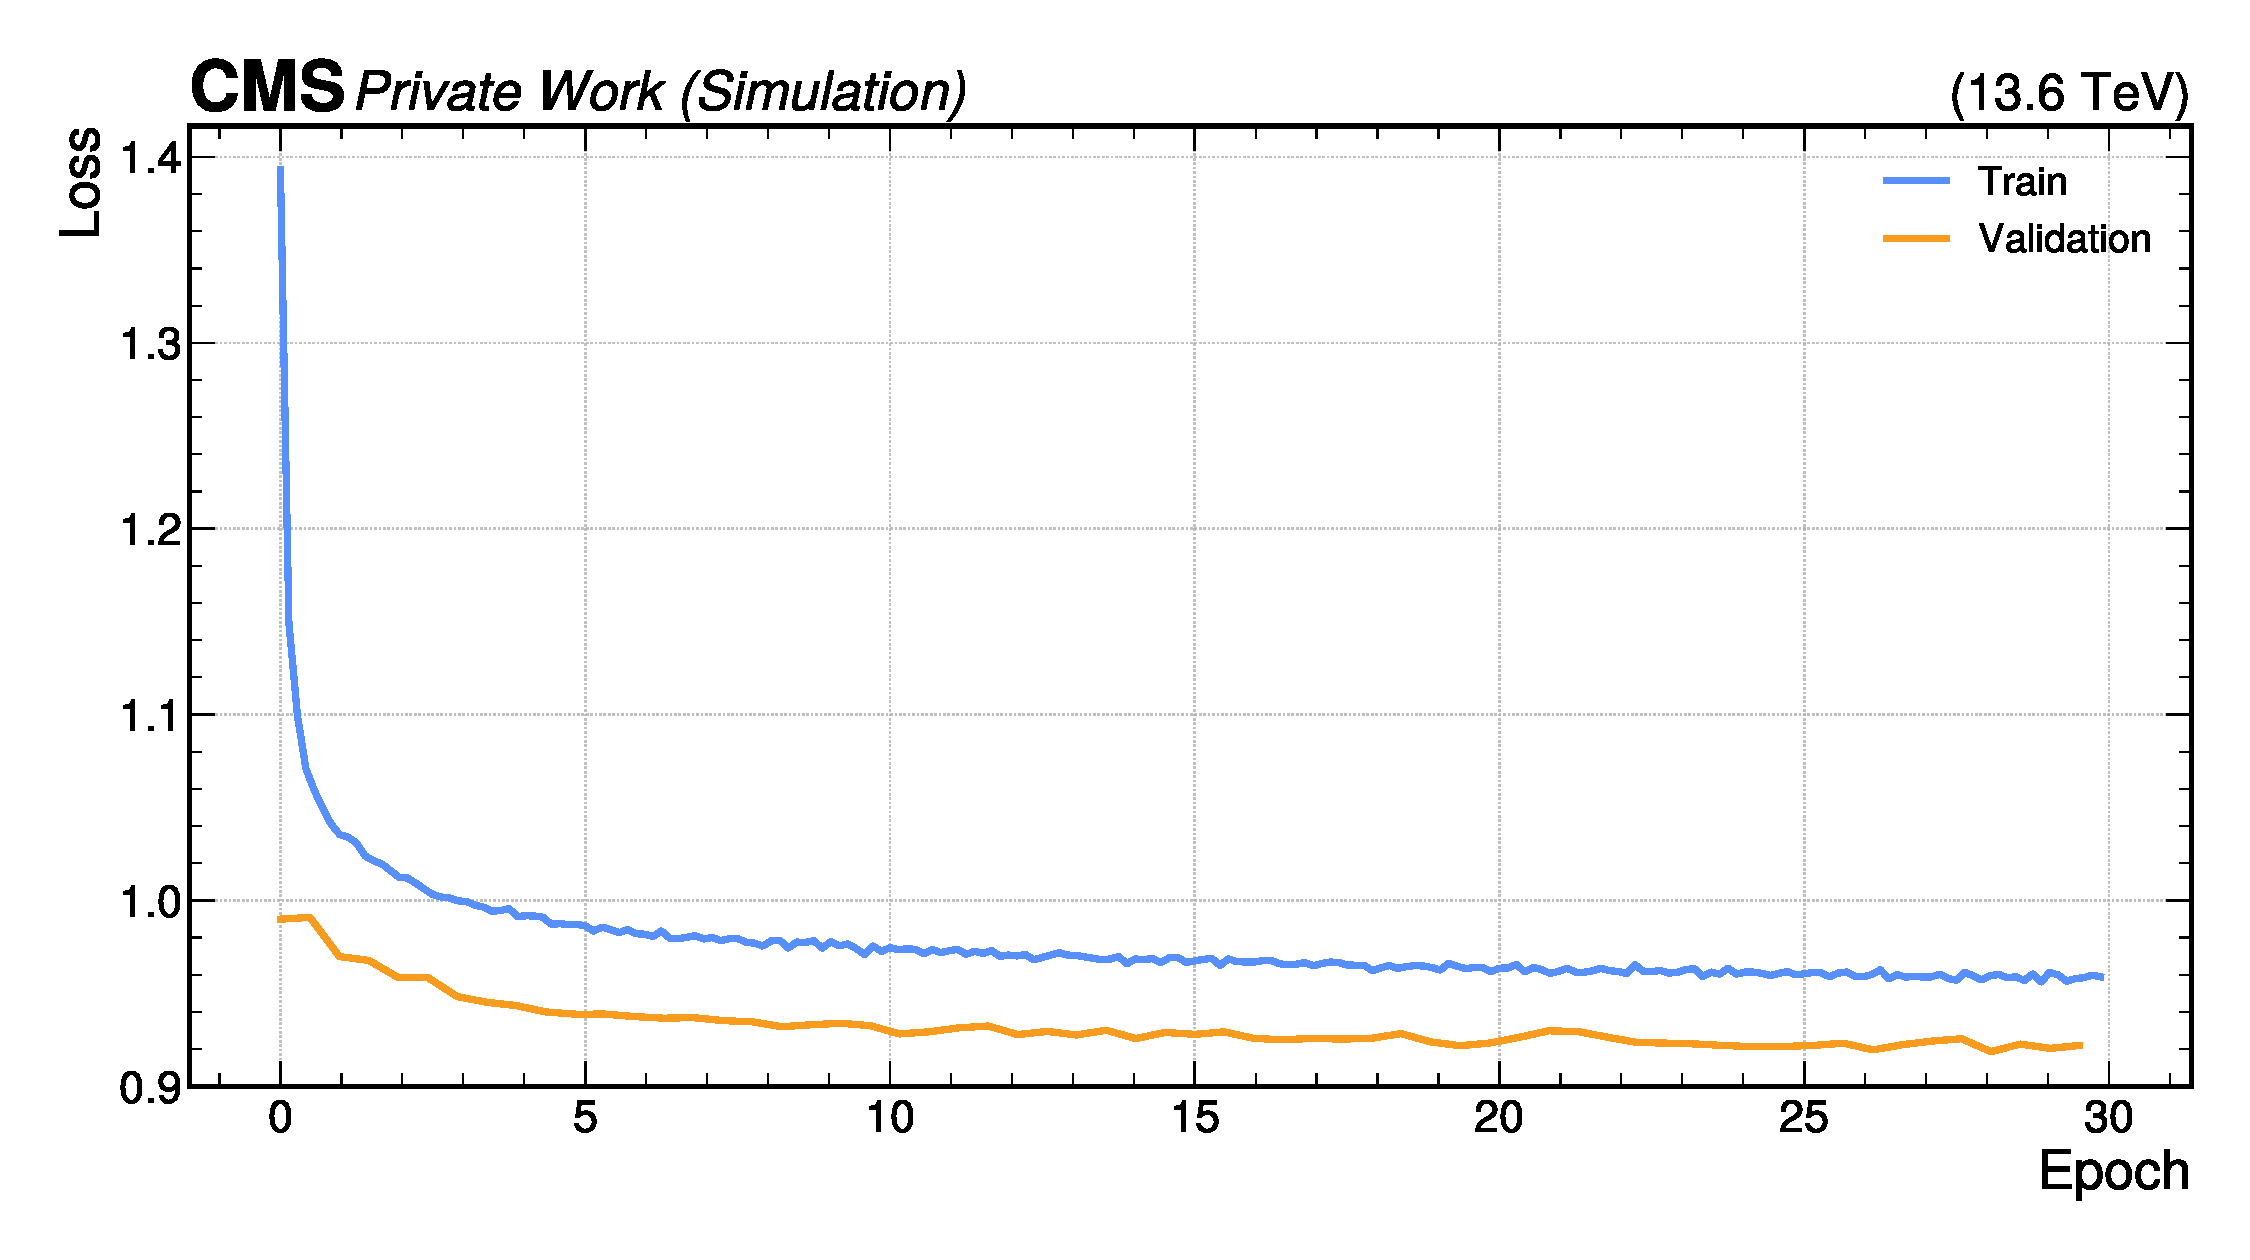
\includegraphics[width=15cm]{media/output/pgd_loss_validation.pdf}
    \caption{Training and validation loss for a PGD(1) trained model with a magnitude of $\epsilon=0.1$ for up to 30 epochs.}
    \label{fig:pgd_loss_curve}
\end{figure}

A PGD trained model offers robustness across PGD inferred data ($AUC=0.955$), while remaining a high AUC score for nominal data ($AUC=0.960$). Compared to the nominal trained model against PGD ($AUC=0.937$), it offers effective defence while staying true nominal performance of ($AUC=0.955$). The corresponding ROC curves are depicted in figure \ref{fig:pgd_trained}. 

\begin{figure}[h]
\centering
    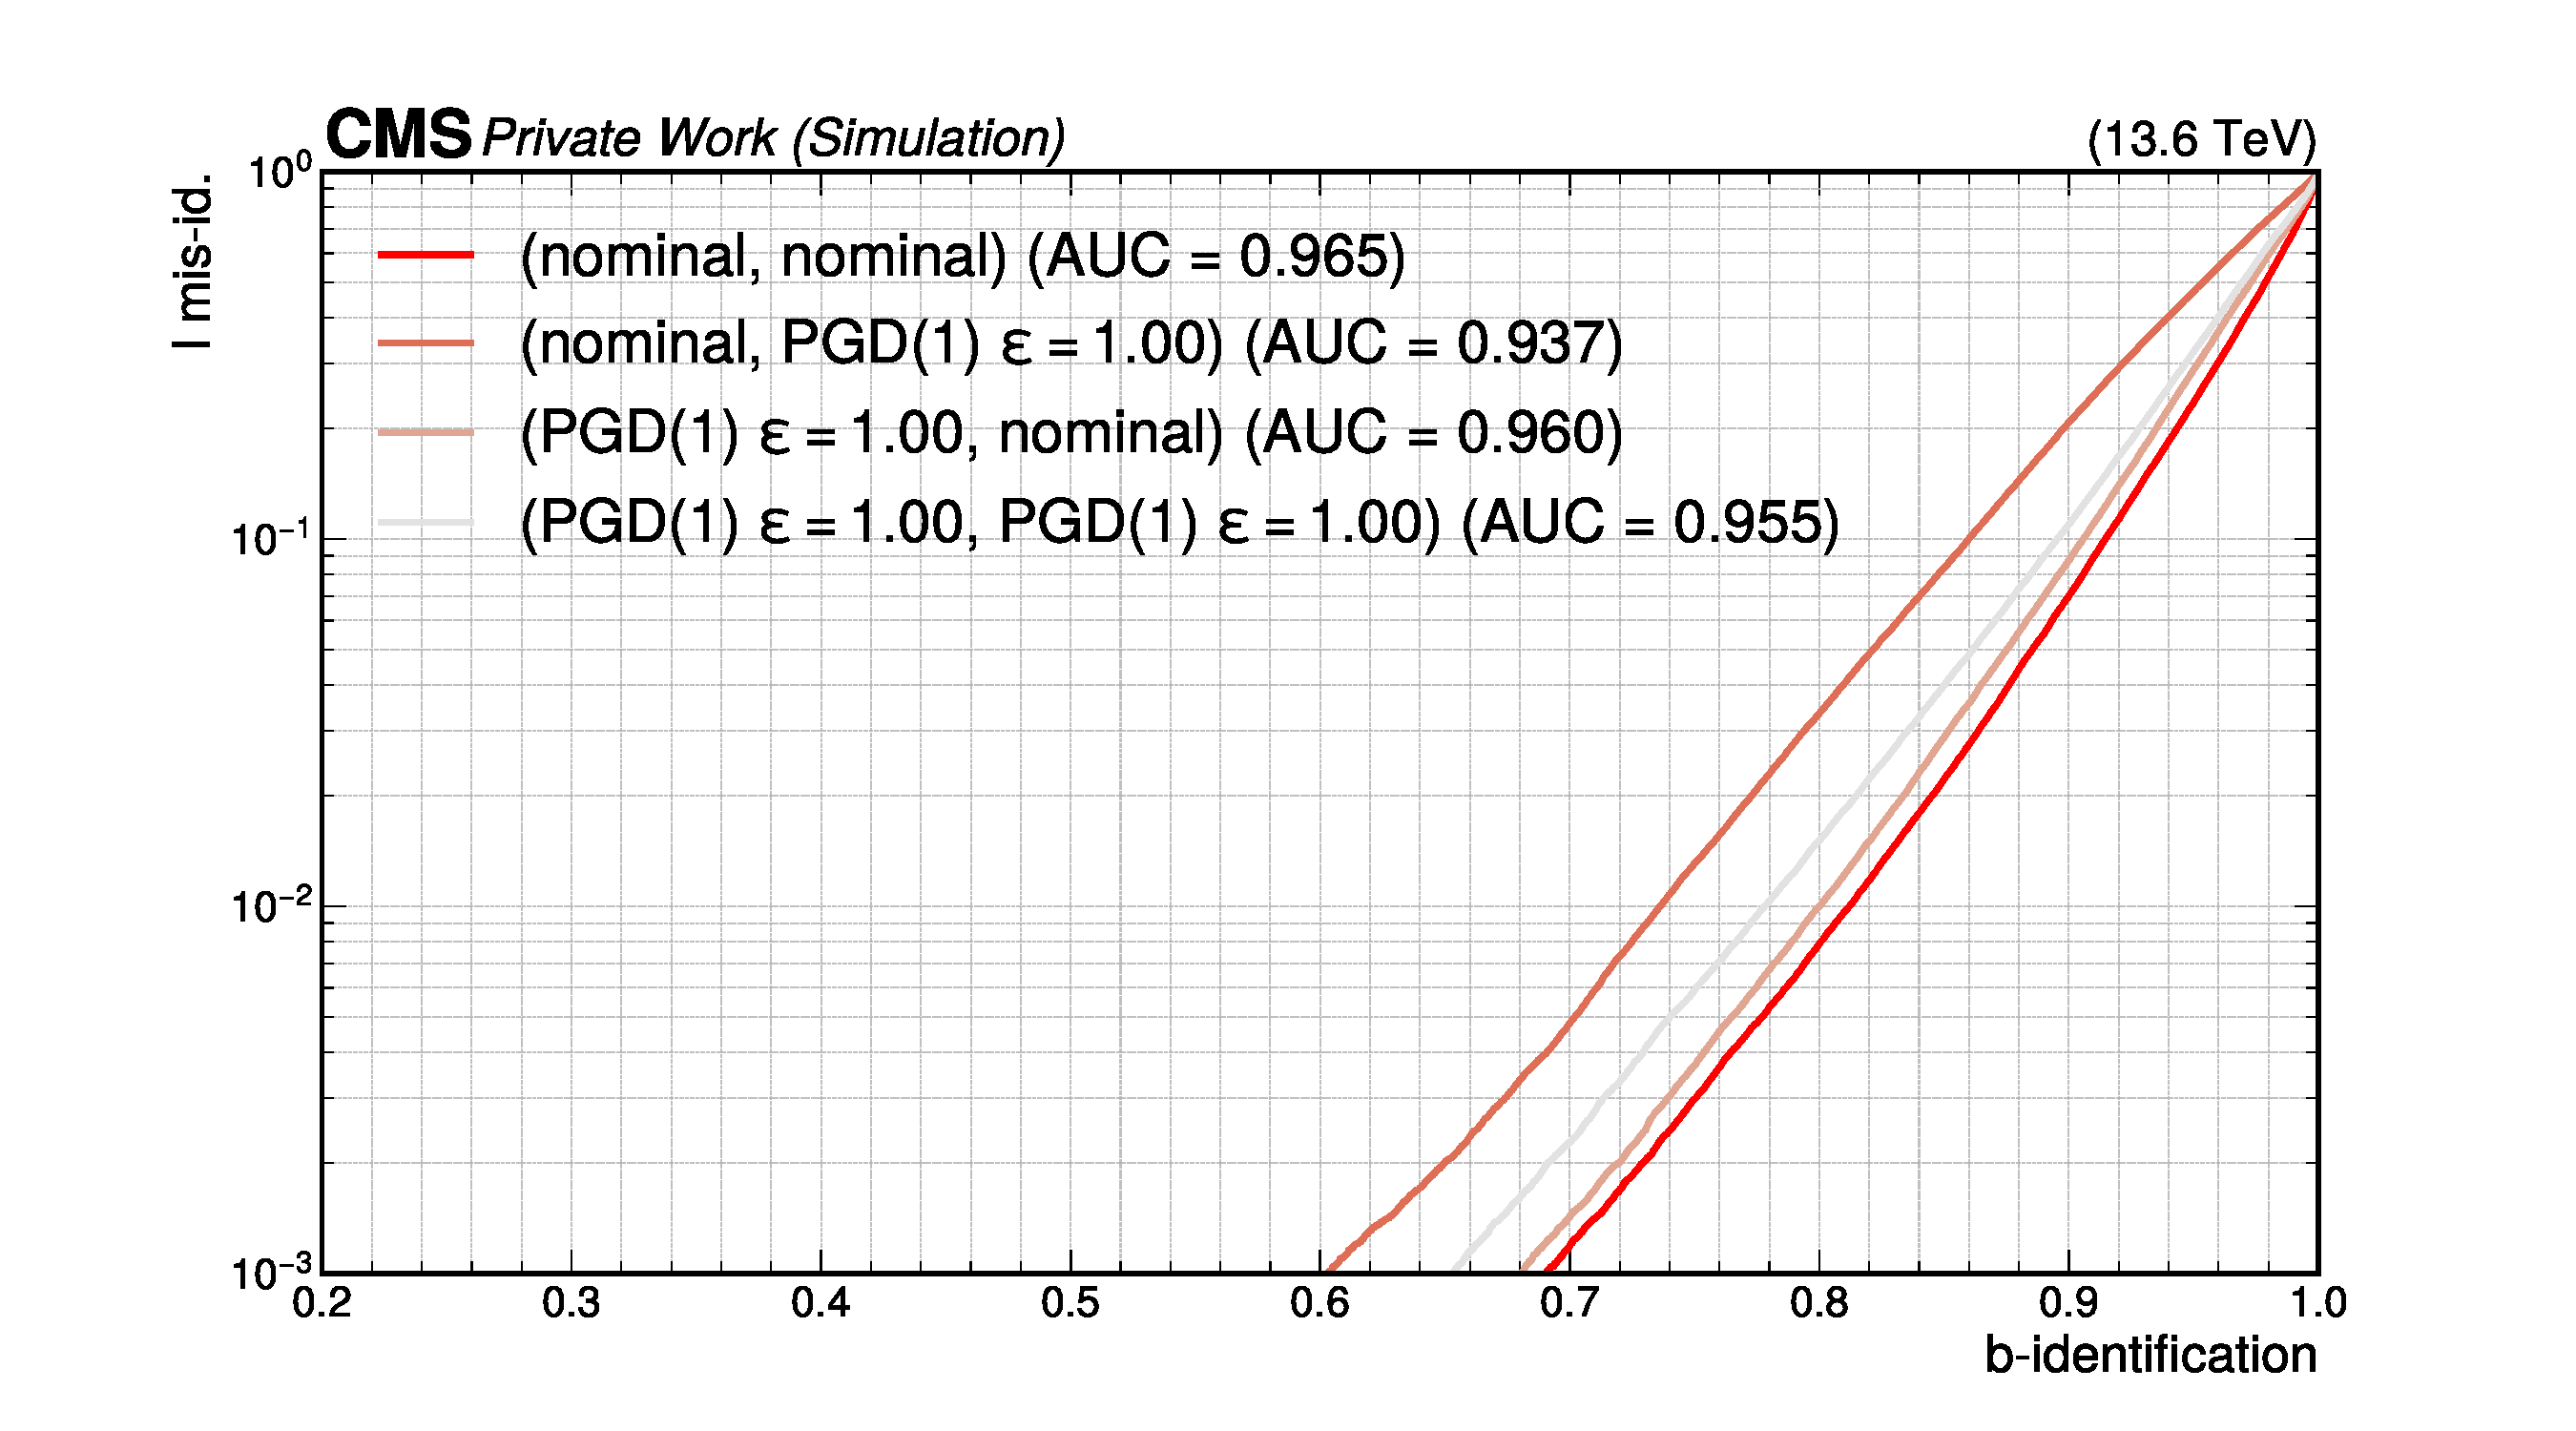
\includegraphics[width=15cm]{media/output/roc_bvsl_pgd_perms.pdf}
    \caption{ROC curves for BvsL misidentification for a PGD(1) and nominal trained model tested against nominal or PGD(1) perturbed inputs with a magnitude of $\epsilon=0.1$.}
    \label{fig:pgd_trained}
\end{figure}

\FloatBarrier
% PIP
\section{Probabilistic Integer Perturbation}
\label{sec:inprob_result}

If not declared specifically a sharpness of $s=1$ is assumed throughout this section. This value was chosen as it represents a compromise between nominal performance and a full-blown attack (see section \ref{sec:intprob_variability} for more details).

\paragraph{Severity:} The stealth characteristics of PIP attacks are fundamentally different from continuous perturbation methods due to their discrete nature. Figures \ref{fig:intprob_joint_overview} illustrates the perturbation severity over the targeted input domain. A comprehensive list of histograms for the input similarity of all features is provided in the Appendix \ref{appendix:intprob}.

The JSD analysis reveals that PIP perturbations maintain higher characteristics compared to PGD, with divergence values typically in the range of $\mathcal{O}(10^{-2})$ and some values going as far as $\mathcal{O}(10^{-1})$. These values occur as PIP is inherently discrete and its impact is generally dependent on the value range of each feature (e.g. for features such as \texttt{Npfcan\_isGamma} — a boolean flag — flipping a bit corresponds to a 100\% change in the respective input domain).

The comparison of single and double-iteration for PIP attacks — as seen in figures \ref{fig:intprob_severity_npv} and \ref{fig:intprob_severity_vtxAss} — indicates a relatively minimal difference in perturbation severity.

\begin{figure}[h]
\centering
    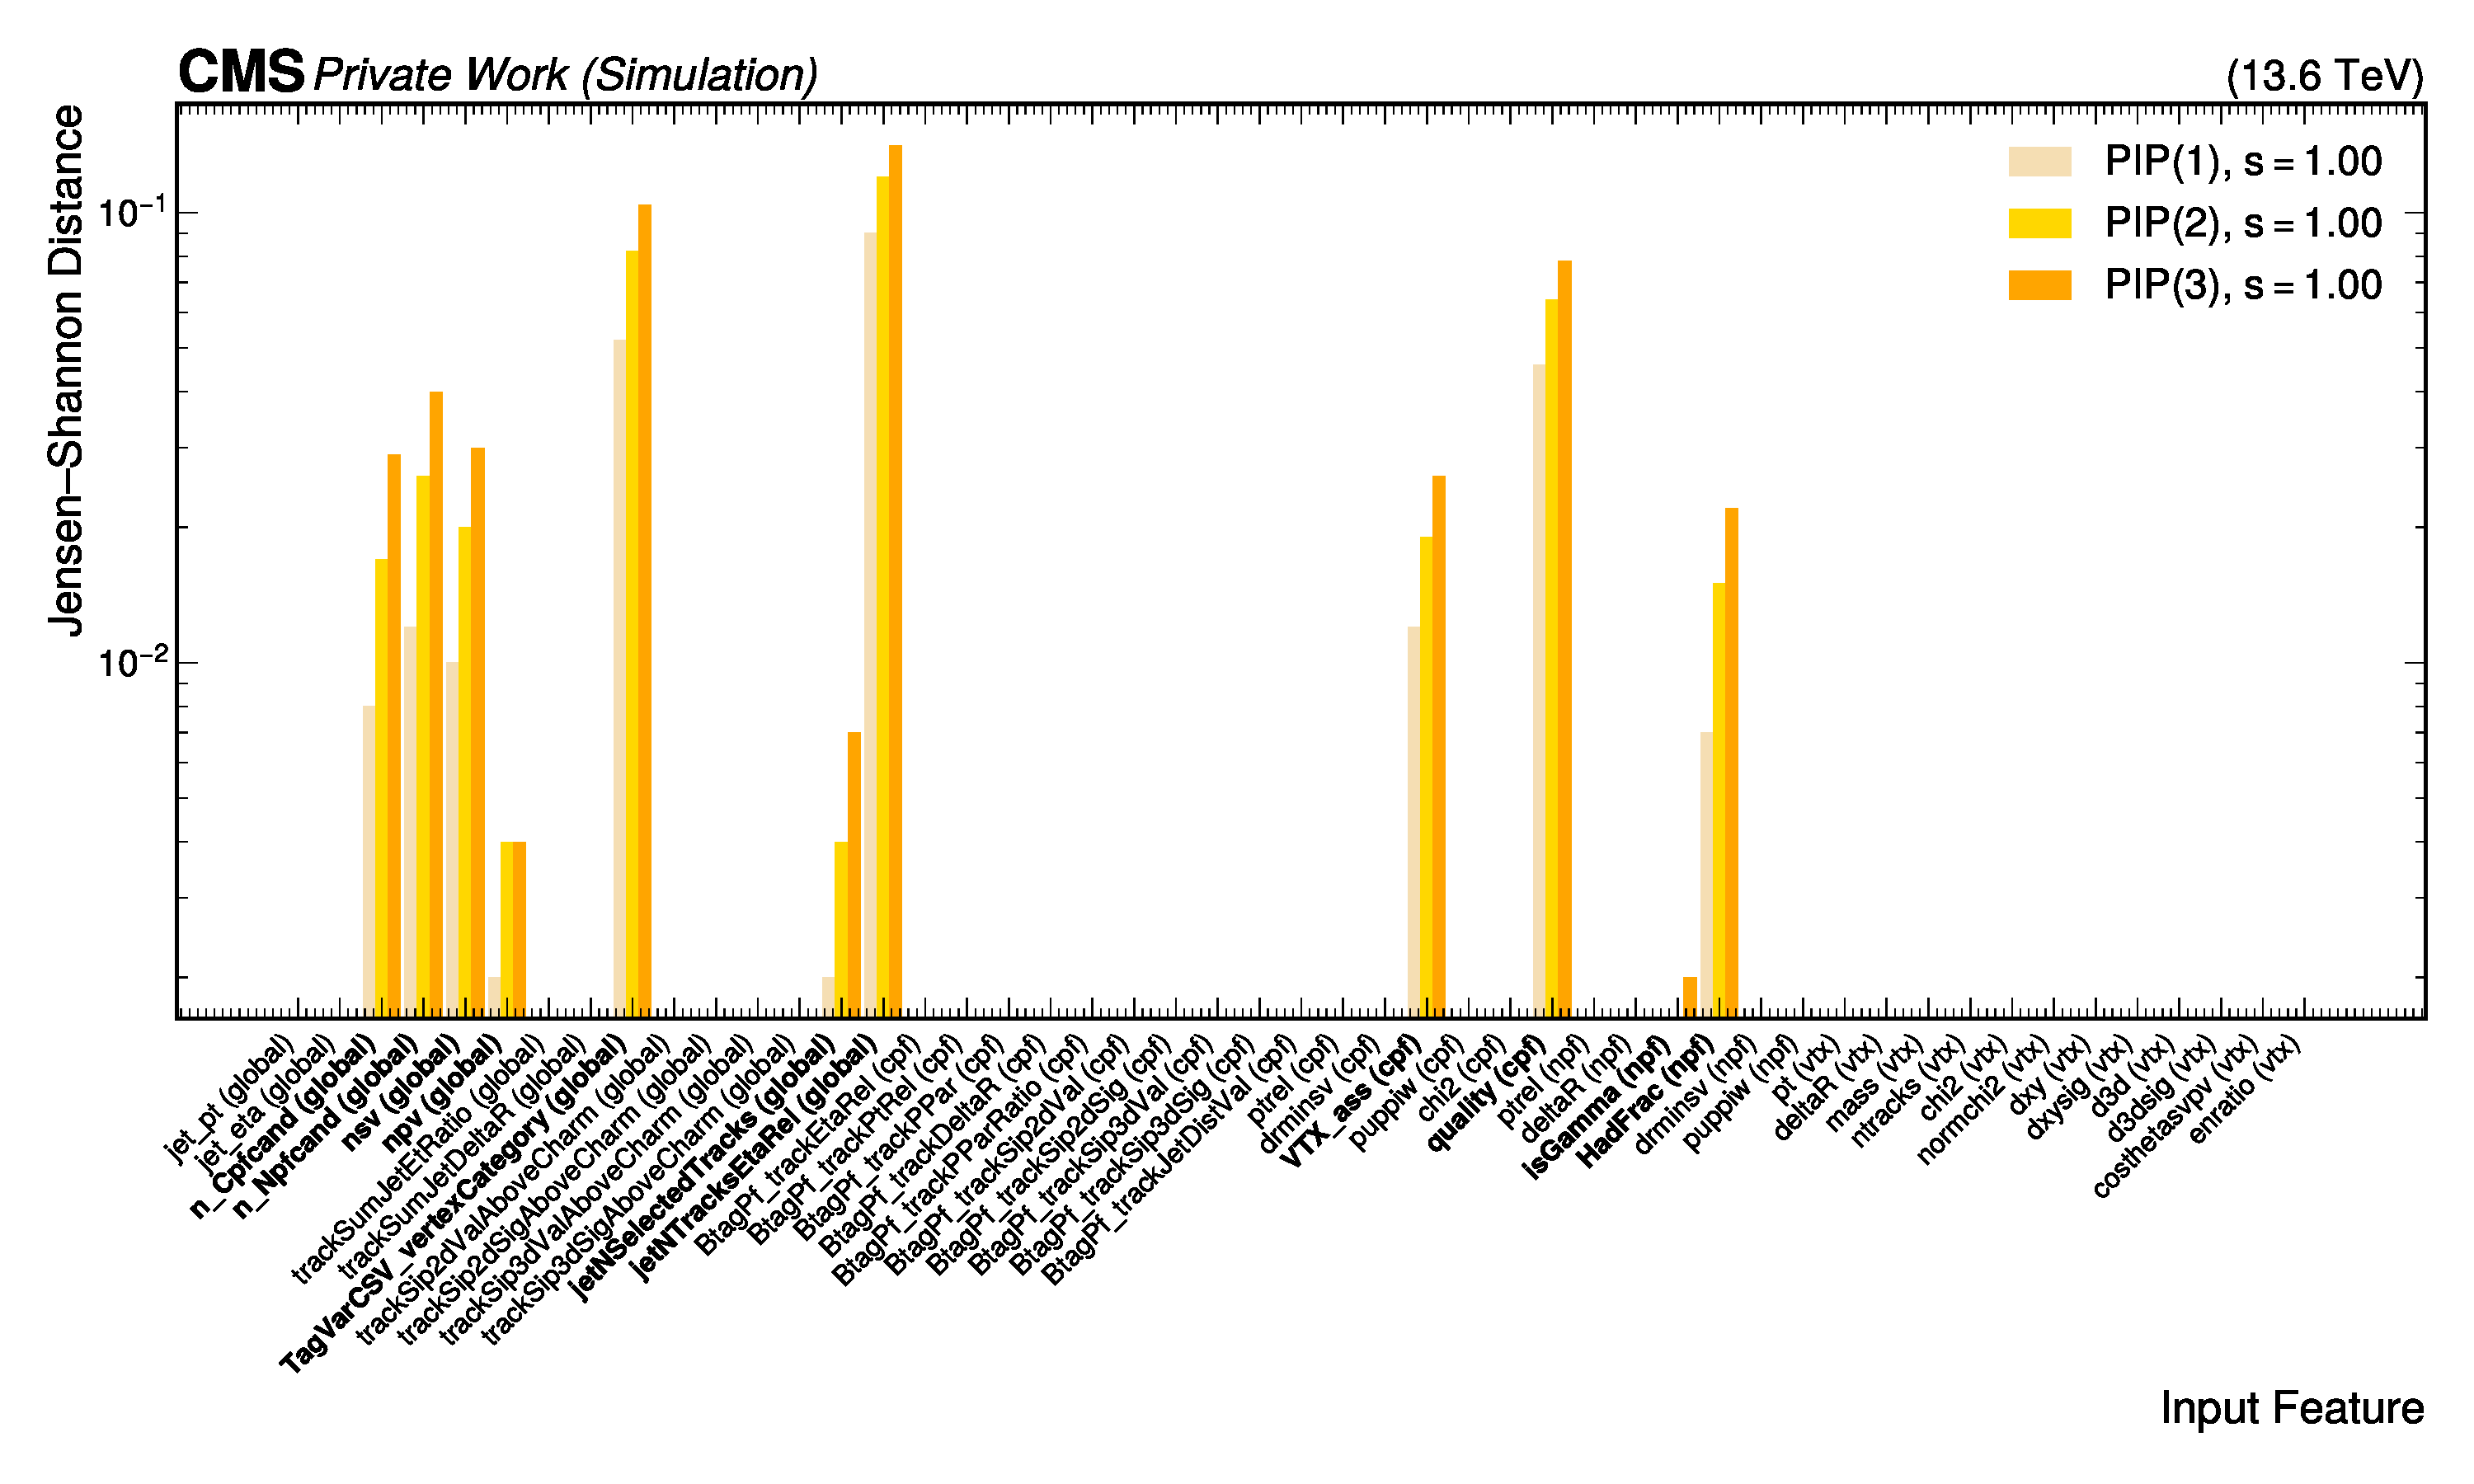
\includegraphics[width=15cm]{media/output/features/compare/jsd_intprob_per_feature.pdf}
    \caption{JSD input similarity development for up to three iterations of the PIP attack with $s=1$ compared against a nominal trained model.}
    \label{fig:intprob_joint_overview}
\end{figure}

\begin{figure}[htbp]
  \centering
  \begin{subfigure}[t]{0.5\textwidth}
    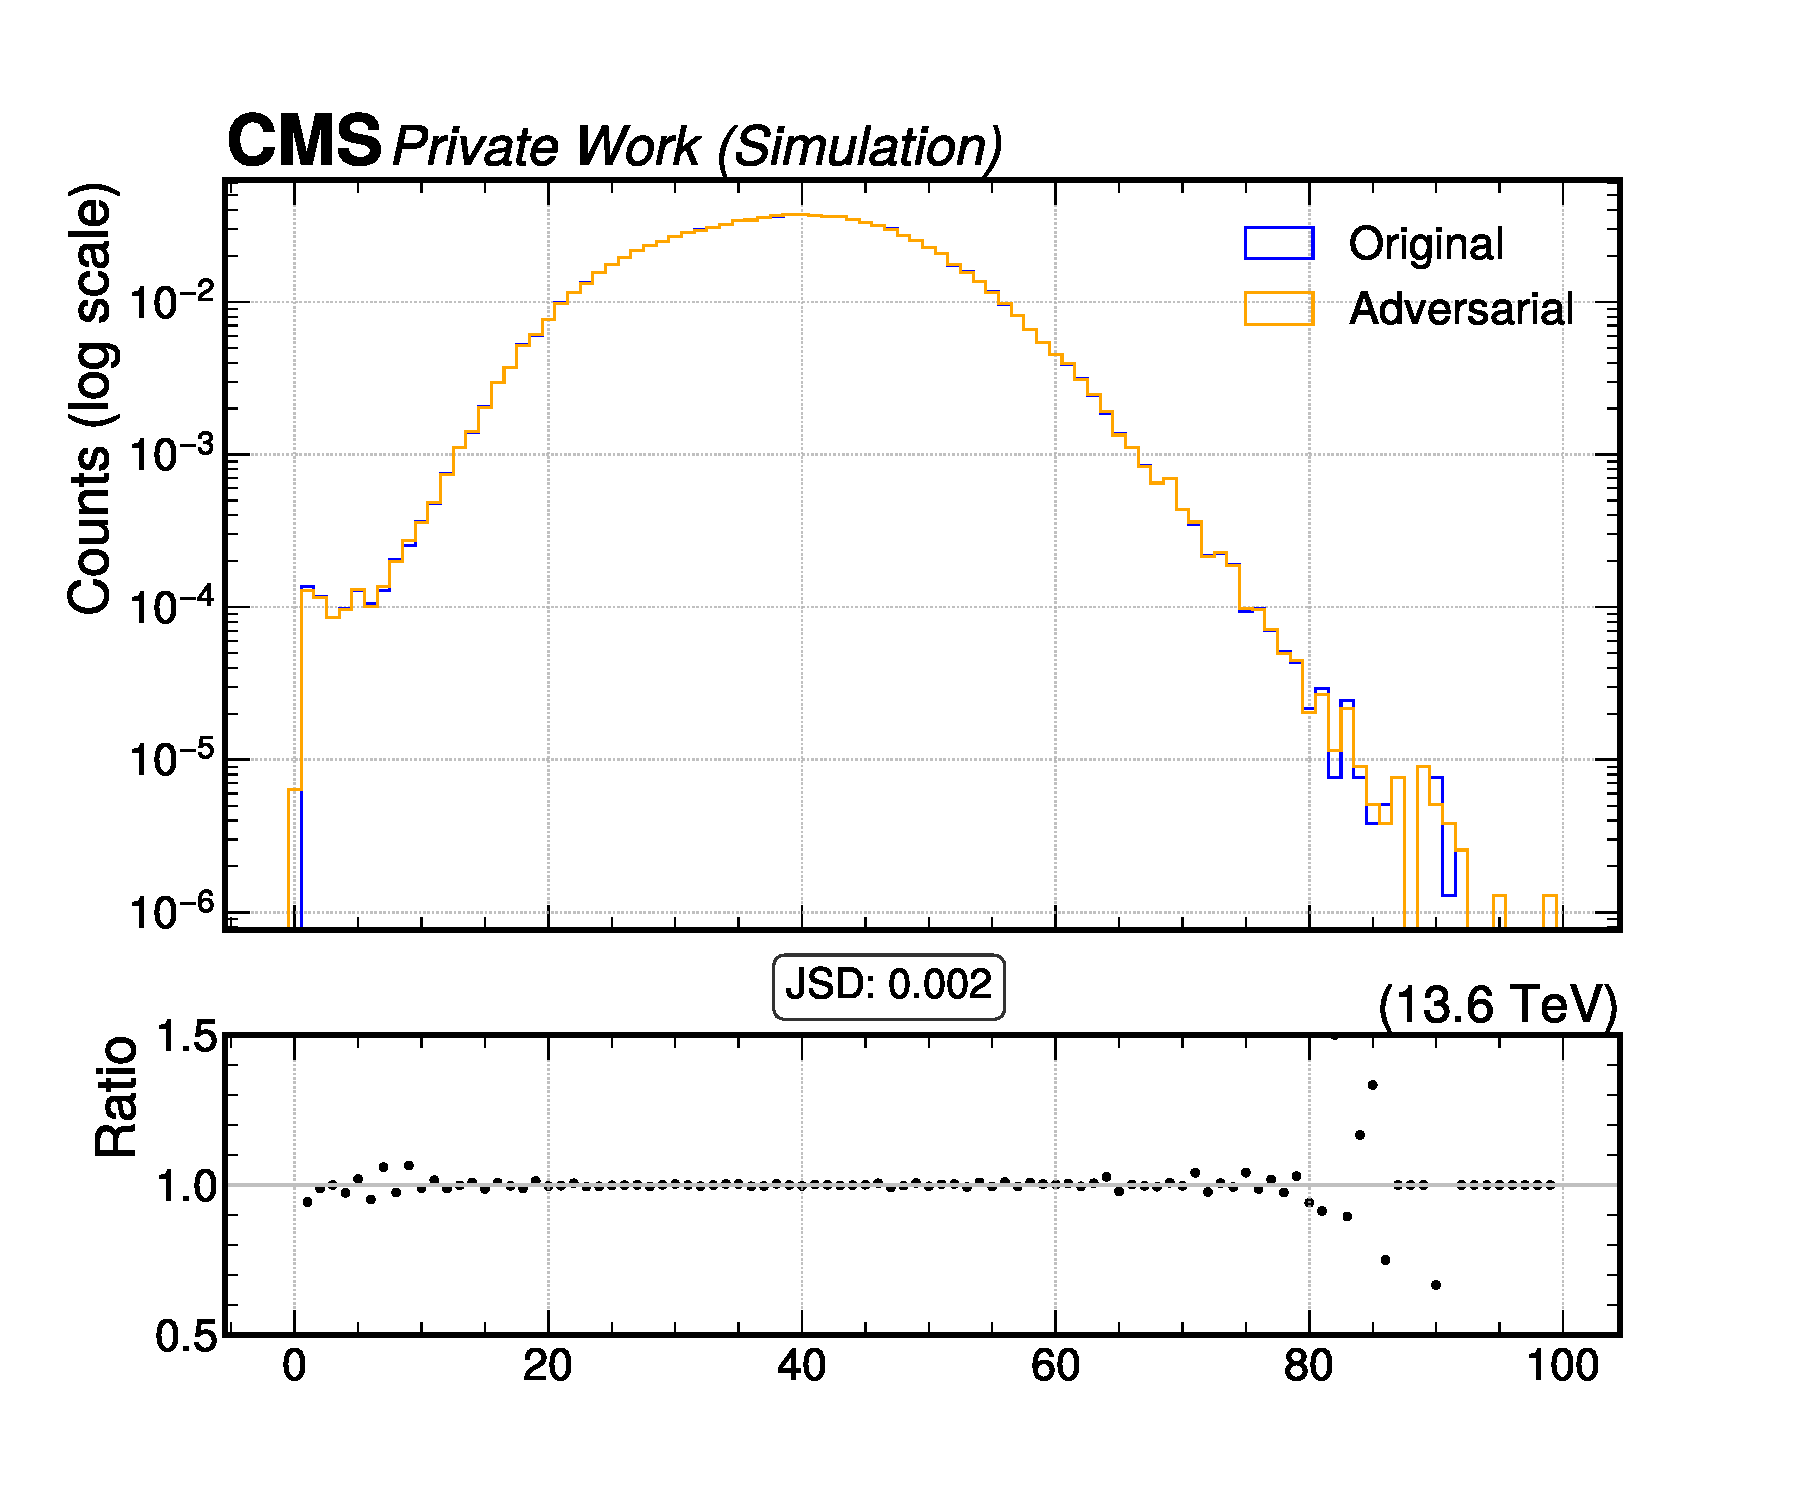
\includegraphics[width=\linewidth]{media/output/features/compare/intprob_1/cmp_global_features_npv.pdf}
    \caption{Input similarity for PIP(1).}
    \label{fig:left}
  \end{subfigure}\hfill
  \begin{subfigure}[t]{0.5\textwidth}
    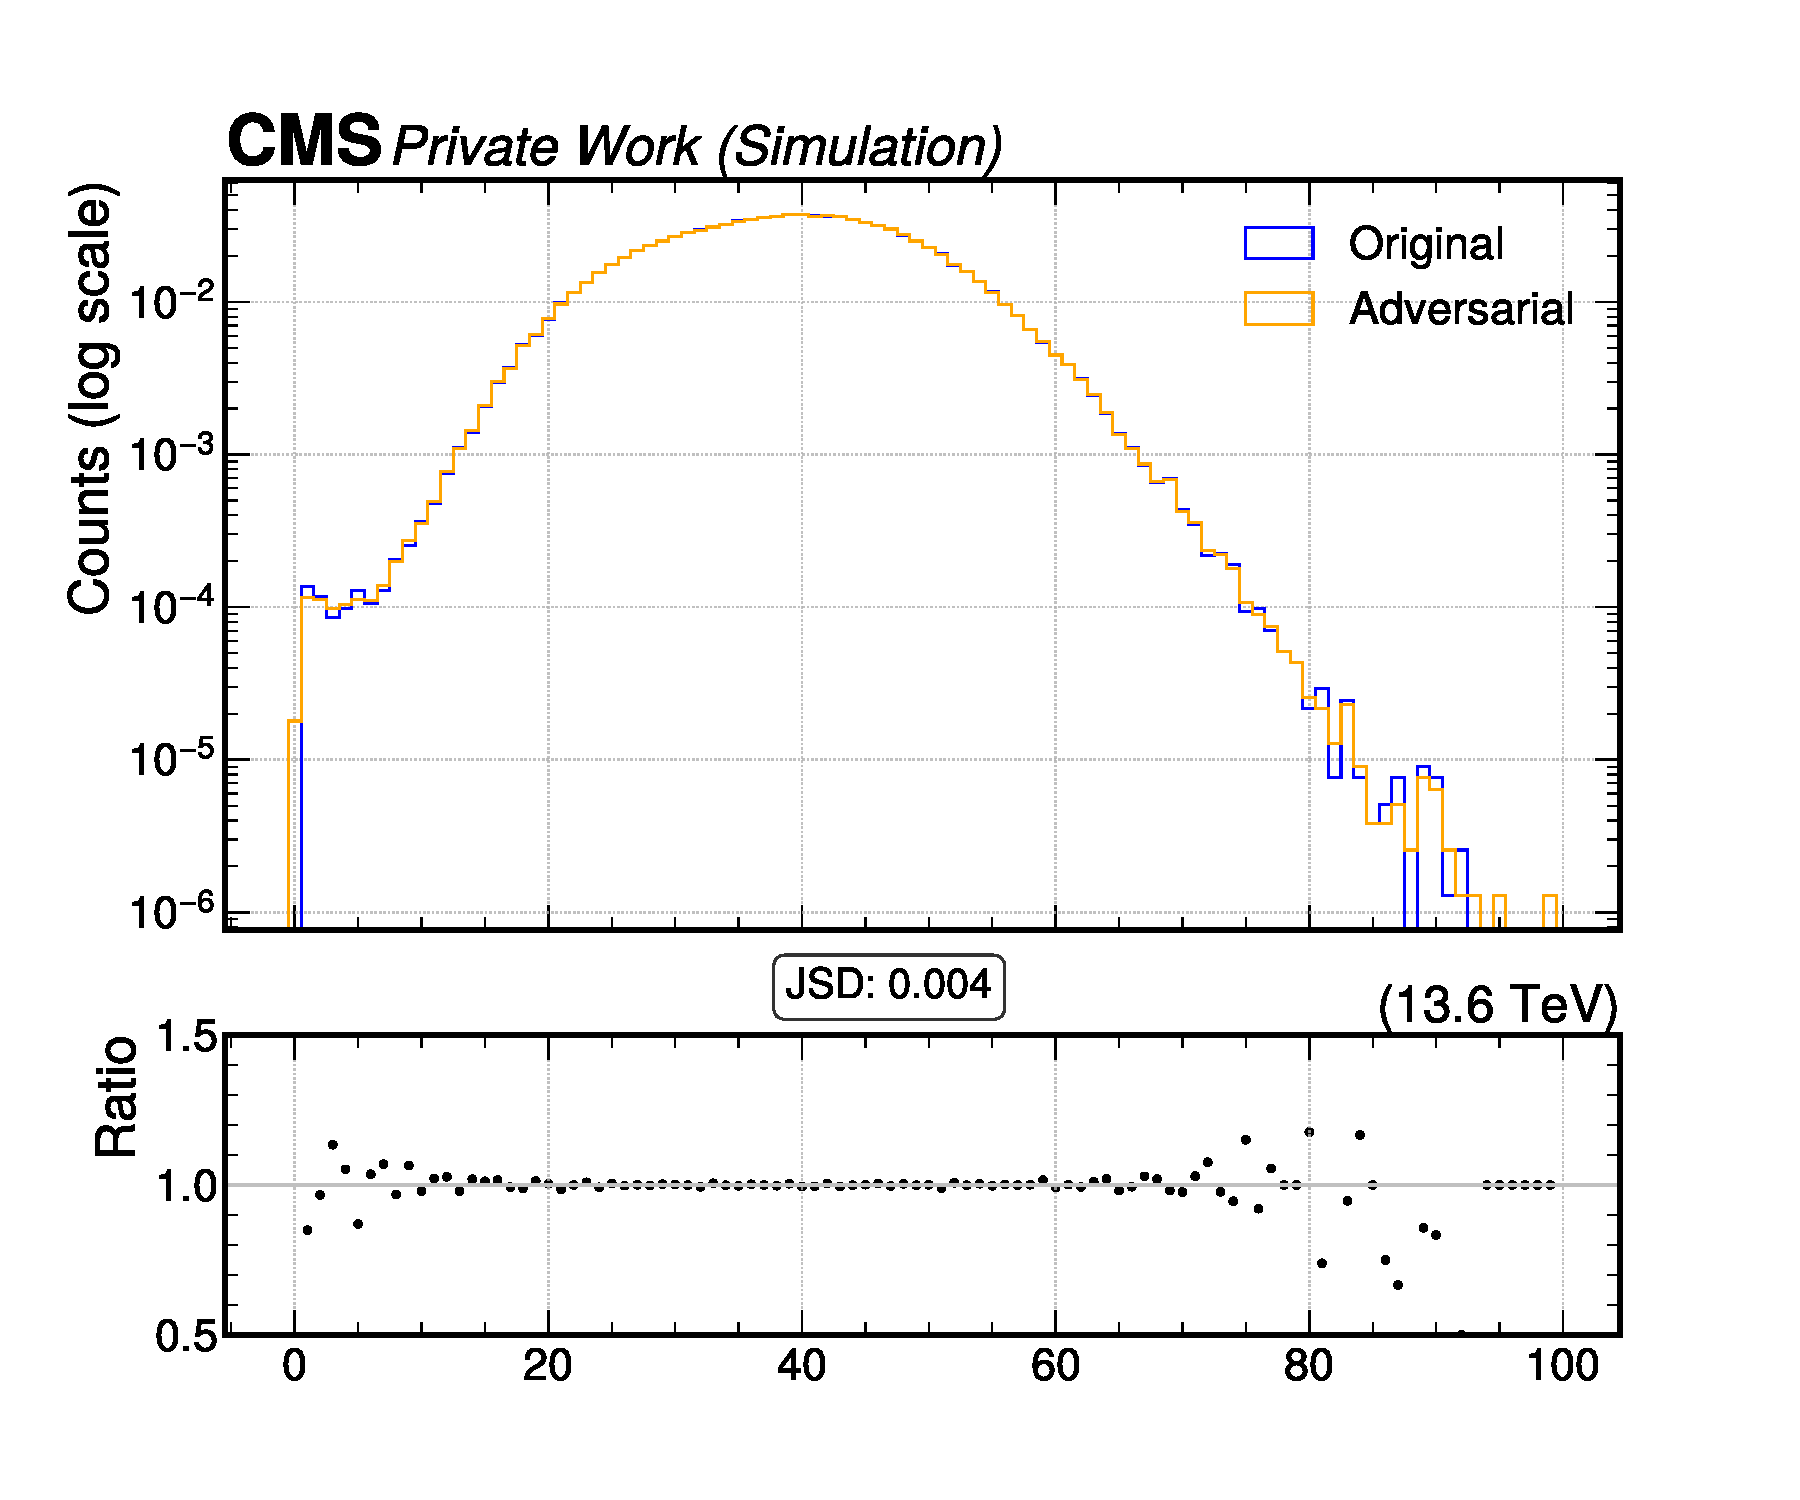
\includegraphics[width=\linewidth]{media/output/features/compare/intprob_2/cmp_global_features_npv.pdf}
    \caption{Input similarity for PIP(2).}
  \end{subfigure}\hfill

  \caption{Histogram for global \texttt{npv} for one and two iterations (left and right respectively) of PIP with a sharpness of $s=1$ compared against nominal inputs.}
  \label{fig:intprob_severity_npv}
  
  \begin{subfigure}[t]{0.5\textwidth}
    \includegraphics[width=\linewidth]{media/output/features/compare/intprob_1/cmp_global_features_nsv.pdf}
    \caption{Input similarity for PIP(1).}
    \label{fig:left}
  \end{subfigure}\hfill
  \begin{subfigure}[t]{0.5\textwidth}
    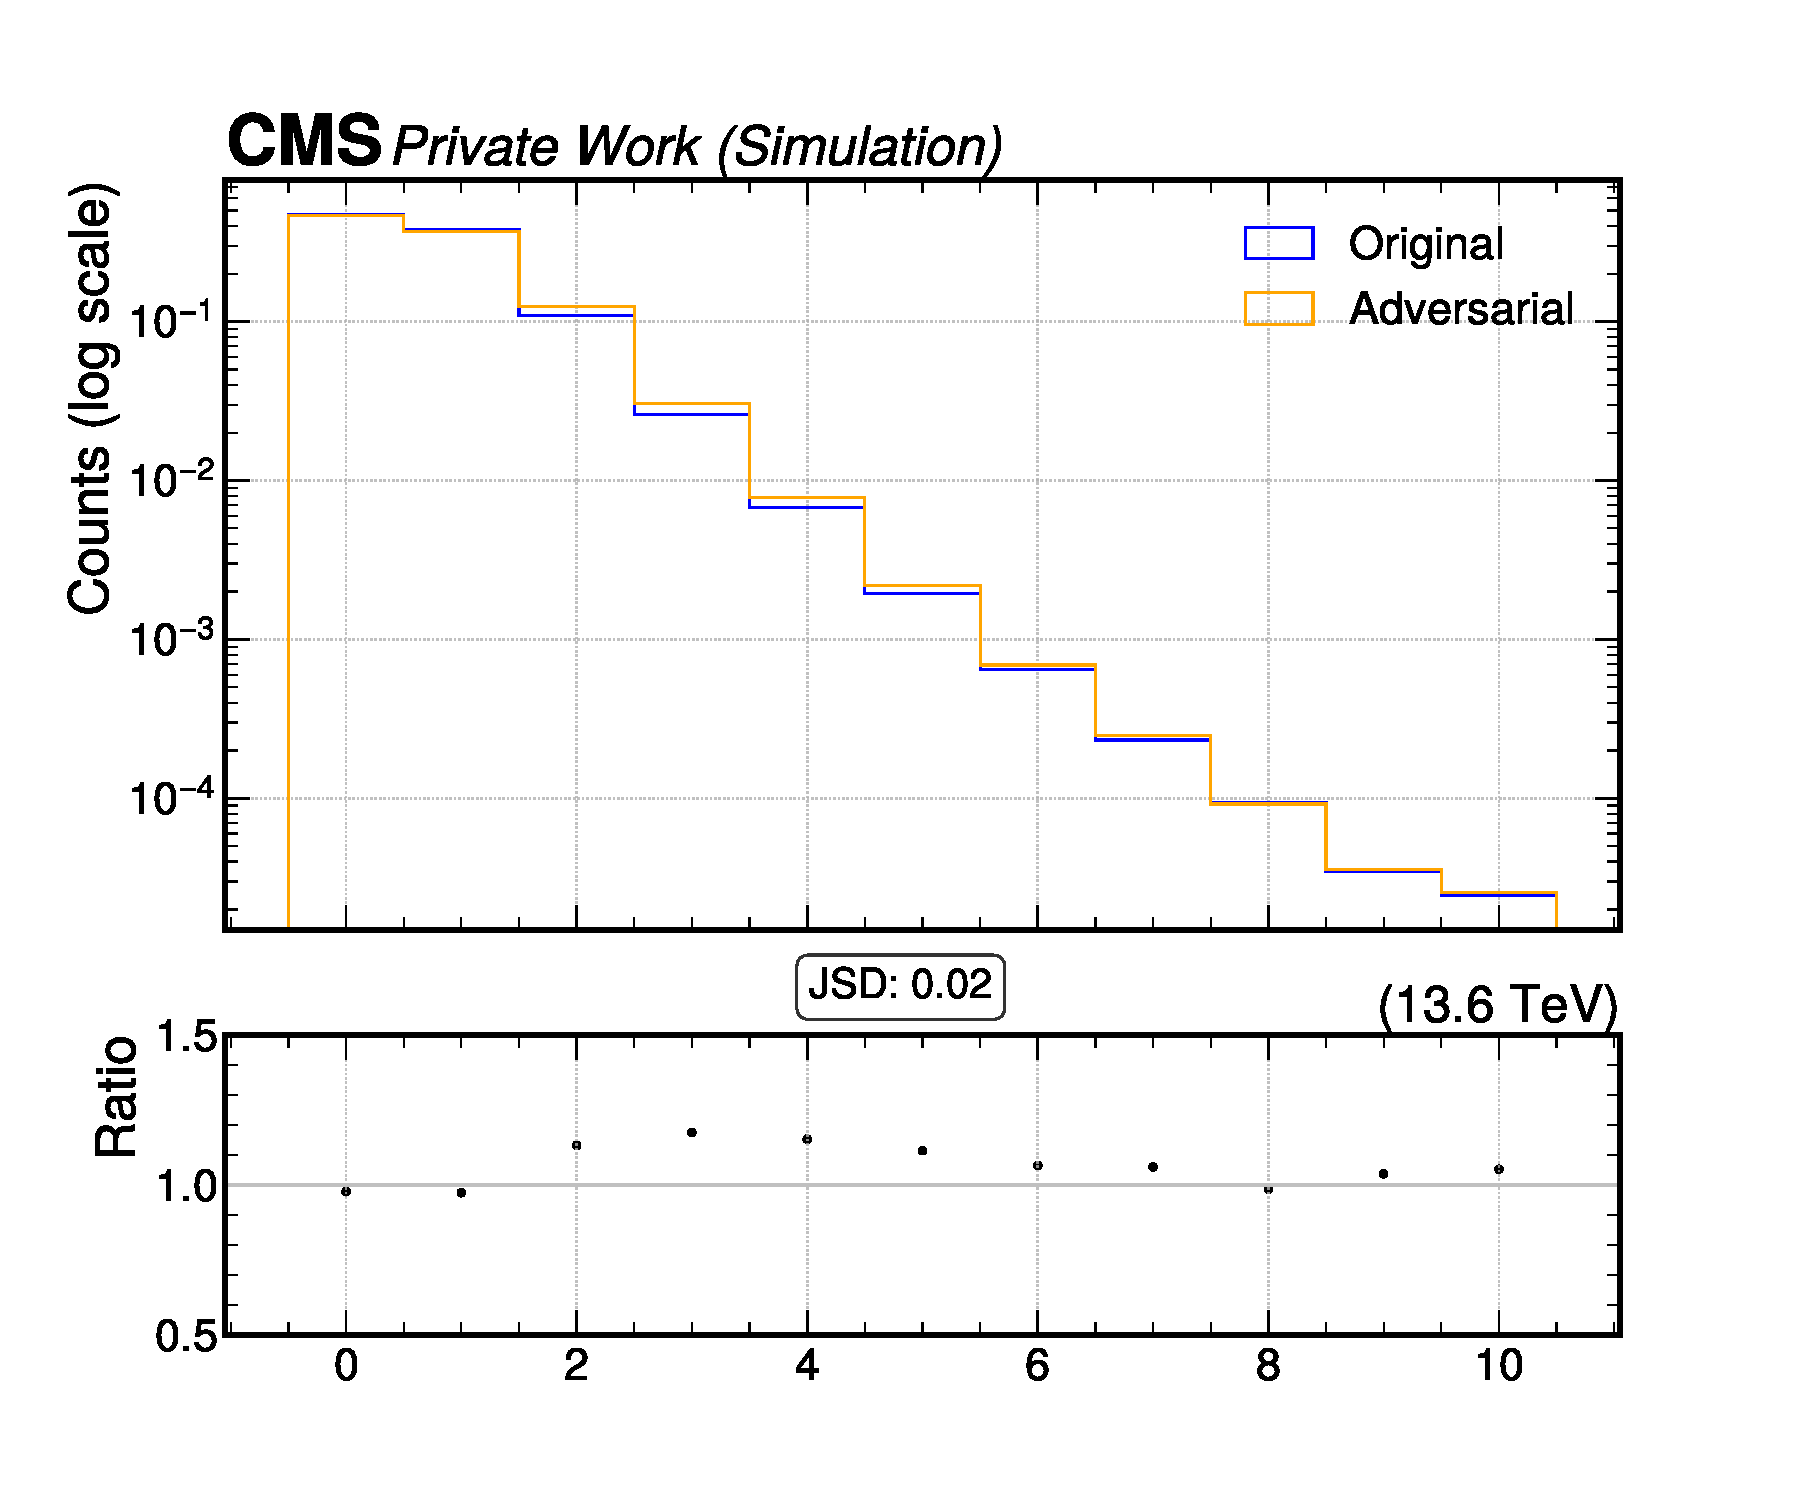
\includegraphics[width=\linewidth]{media/output/features/compare/intprob_2/cmp_global_features_nsv.pdf}
    \caption{Input similarity for PIP(2).}
  \end{subfigure}\hfill

  \caption{Histogram for global \texttt{nsv} for one and two iterations (left and right respectively) of PIP with a sharpness of $s=1$ compared against nominal inputs.}
  \label{fig:intprob_severity_vtxAss}
\end{figure}

\newpage
\paragraph{Attack:} The PIP attack exhibits a distinct characteristic compared to PGD. Its effectiveness depends on the number of iterations and the sharpness parameter in roughly same parts. Figure \ref{fig:intprob_rocs_vs_sharpness} illustrates this relationship, showing how varying sharpness values affect the attack's ability to compromise the classifier:

\begin{figure}[H]
\centering
    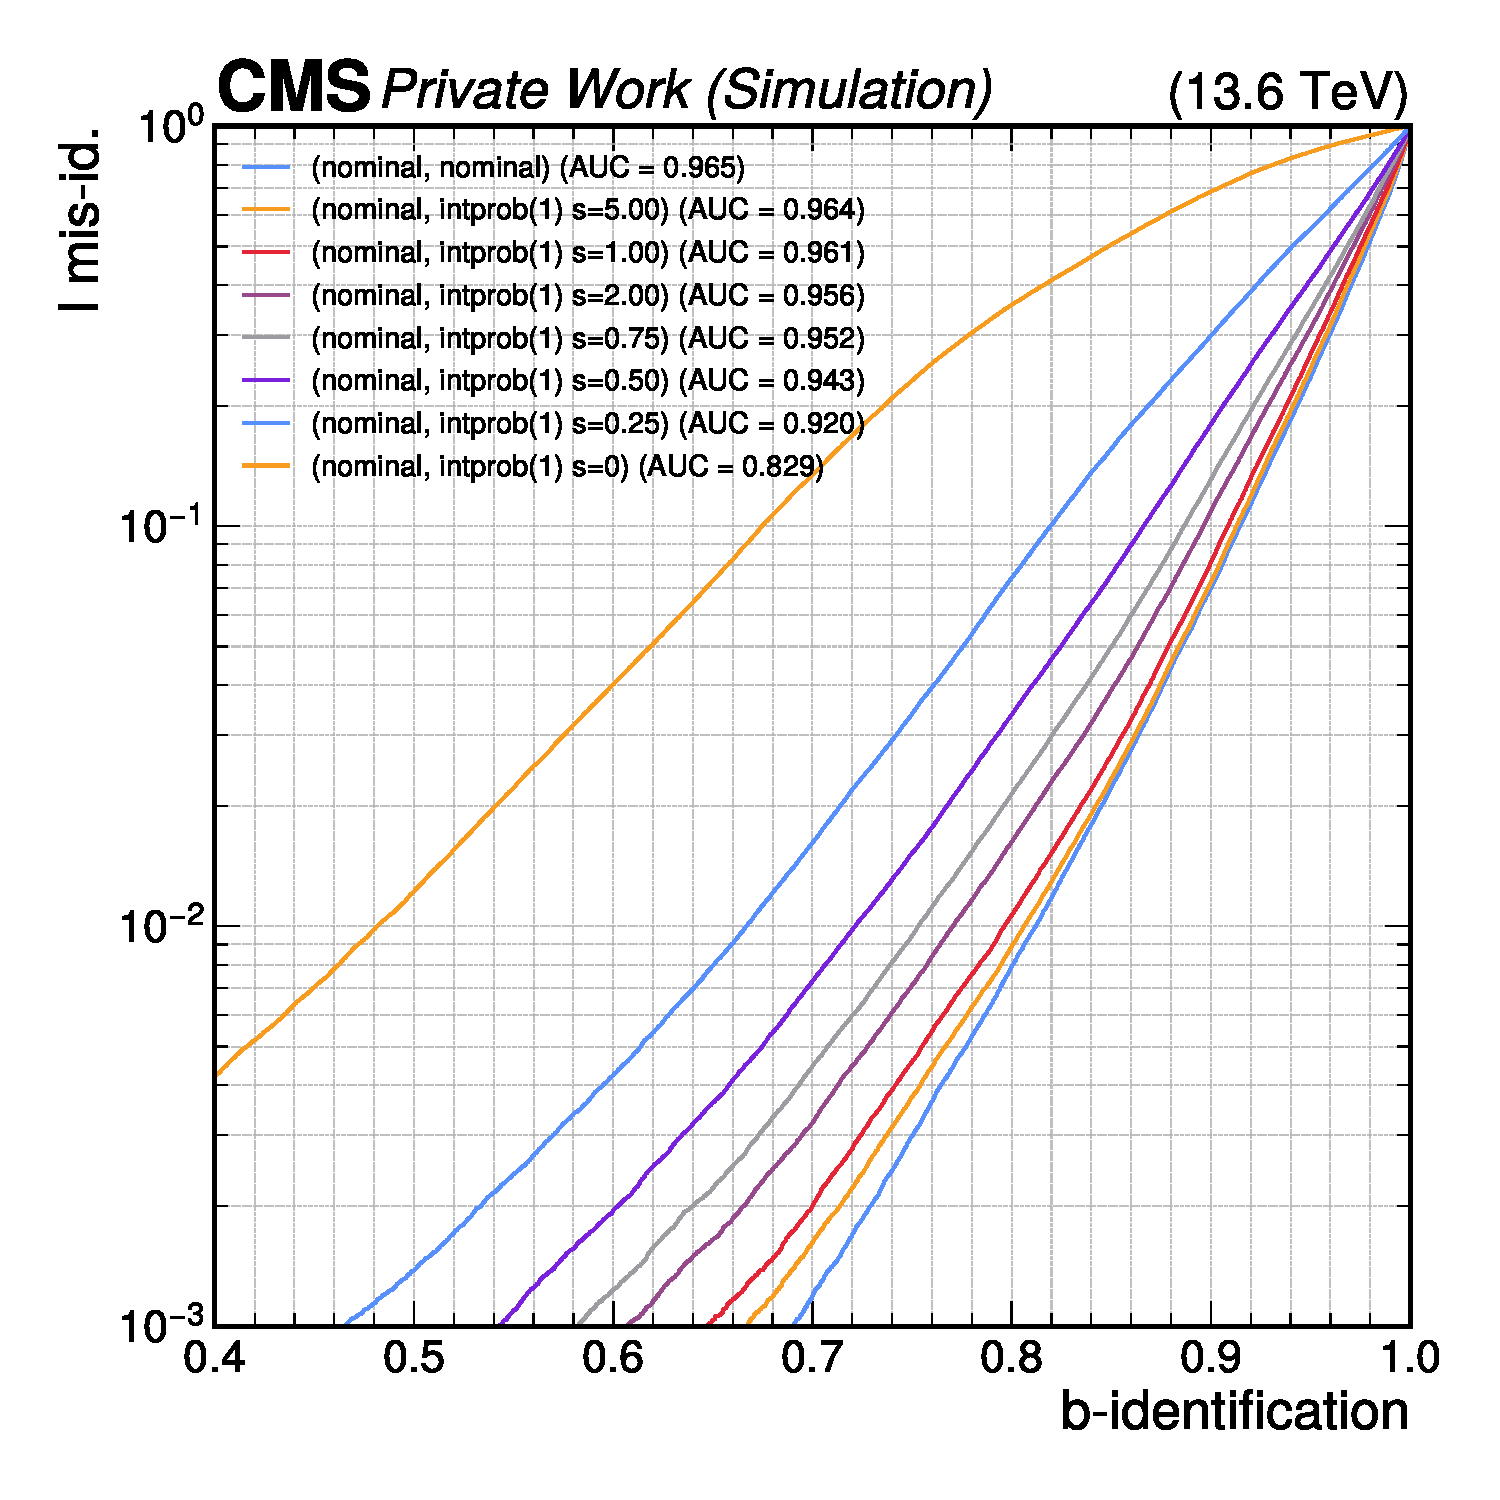
\includegraphics[width=15cm]{media/output/roc_bvsl_intprob_sharpness.pdf}
    \caption{ROC curves for BvsL misidentification of the nominal trained model tested against different sharpness values for the PIP attack at one iteration.}
    \label{fig:intprob_rocs_vs_sharpness}
\end{figure}

\begin{itemize}
    \item At \textbf{high sharpness} ($s = 5$), the attack exhibits minimal impact, with AUC values remaining close to the nominal baseline. This reflects the probabilistic nature of the PIP method—when the sharpness is high, the probability of flipping integer features remains small, resulting in perturbations that are too subtle to significantly affect the classifier's decision boundaries.
    \item At \textbf{moderate sharpness} around $s = 1.0$, a more pronounced degradation becomes apparent, with the AUC dropping to approximately 0.961. This represents the sweet spot where the attack achieves meaningful perturbation while maintaining reasonable stealth characteristics. 
    \item A \textbf{low sharpness} of $s = 0$ corresponds to a completely deterministic attack, where all features with a gradient unequal to zero get eventually increased/decreased. It produces the most aggressive attack, reaching an AUC of around 0.829.
\end{itemize}


Likewise, figure \ref{fig:intprob_rocs_vs_iterations} highlights PIP's iterative behaviour. Unlike PGD, where additional iterations yield progressively smaller changes, PIP exhibits steady AUC degradation, with subsequent iterations reducing the AUC from 0.956 at one iteration to 0.916 at five iterations. This behaviour arises from PIP's stochastic nature, where features unaltered in prior iterations gain further opportunities for modification in later ones. This increases their cumulative perturbation probability across iterations.


\begin{figure}[h]
\centering
    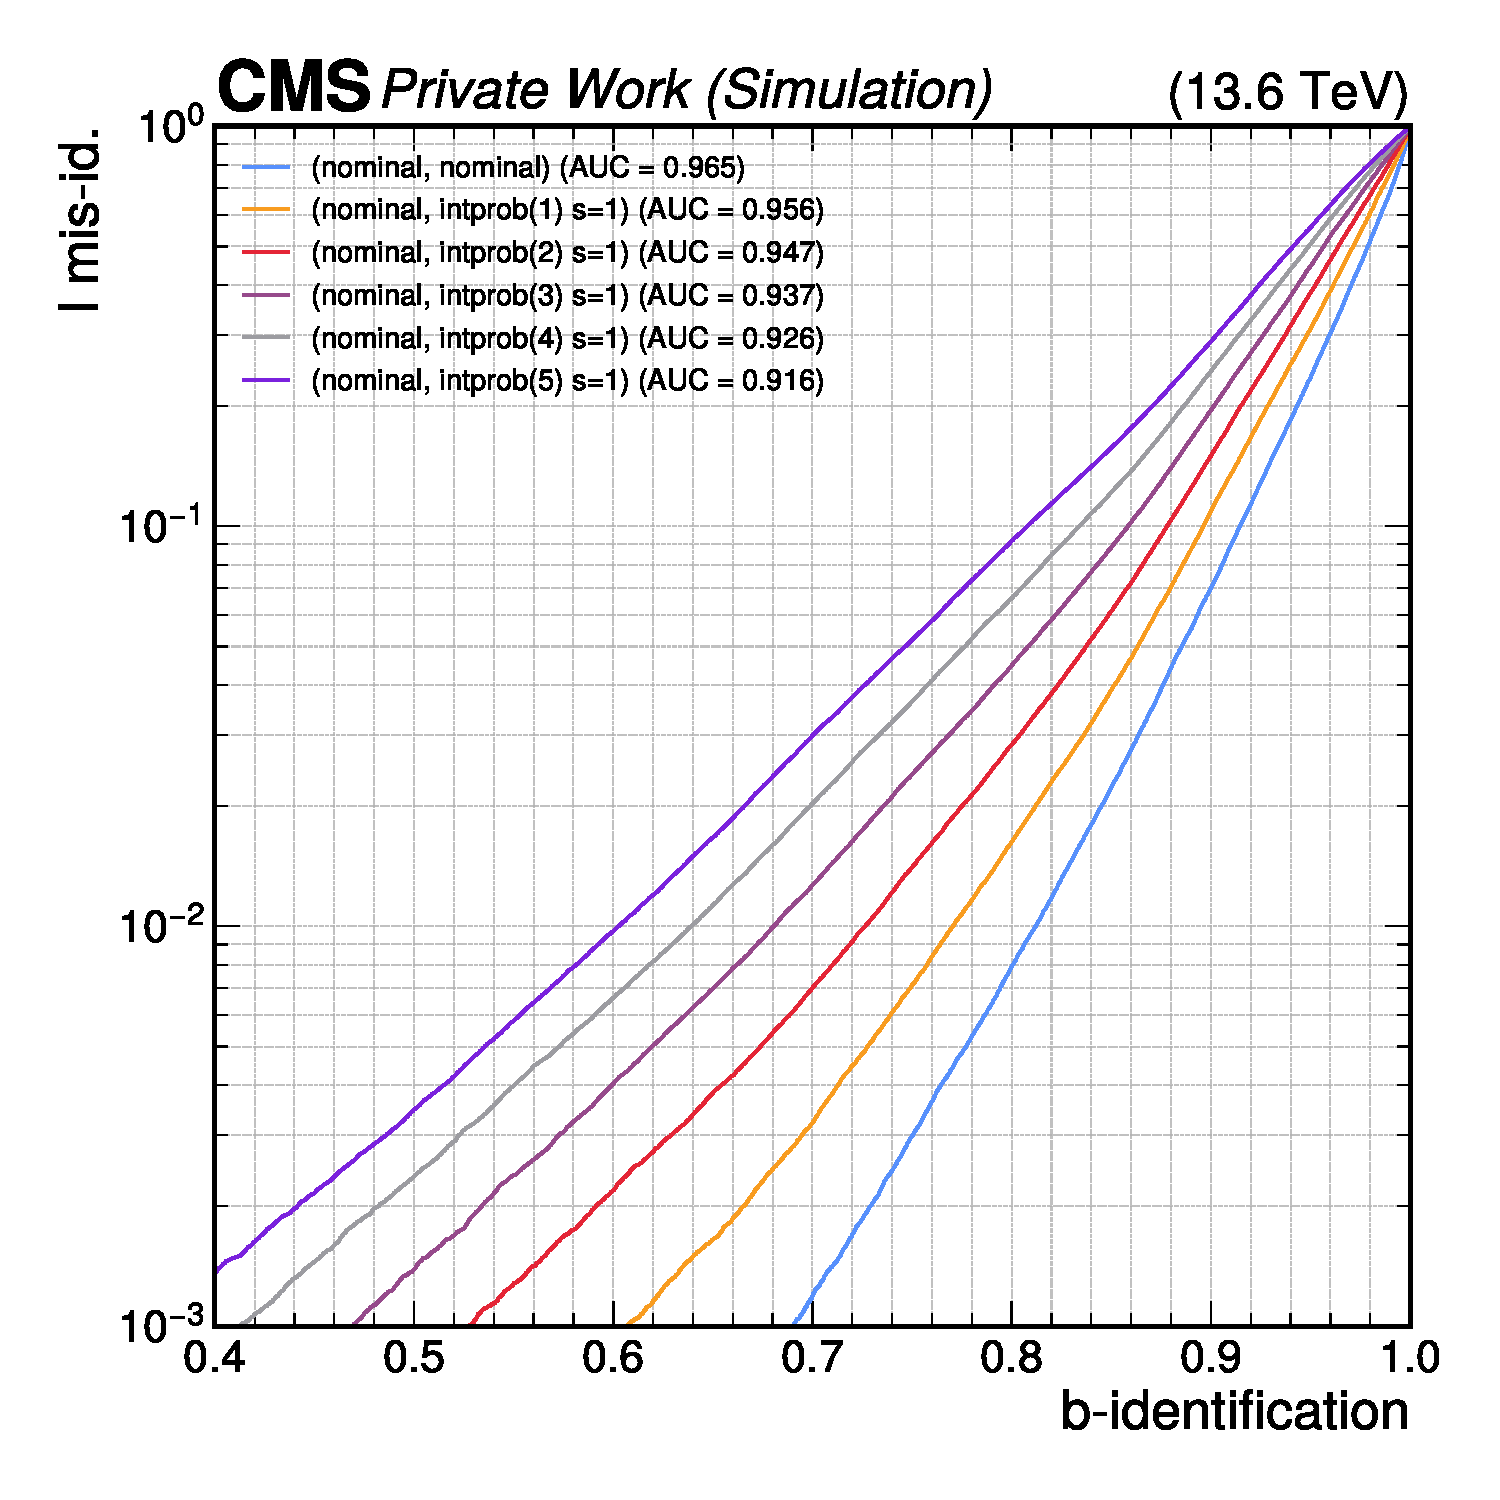
\includegraphics[width=15cm]{media/output/roc_bvsl_intprob_iterations.pdf}
    \caption{ROC curve for BvsL misidentification of the nominal trained model tested against up to five iteration of the PIP attack at $s=1$.}
    \label{fig:intprob_rocs_vs_iterations}
\end{figure}

\paragraph{Adversarial Training:} PIP's adversarial training presents a distinct learning scenario compared to continuous perturbation methods. 
Figure \ref{fig:intprob_training} shows the training dynamics for PIP with sharpness $s=1$ over 30 epochs, revealing several interesting characteristics of discrete adversarial training.

\begin{figure}[h]
\centering
    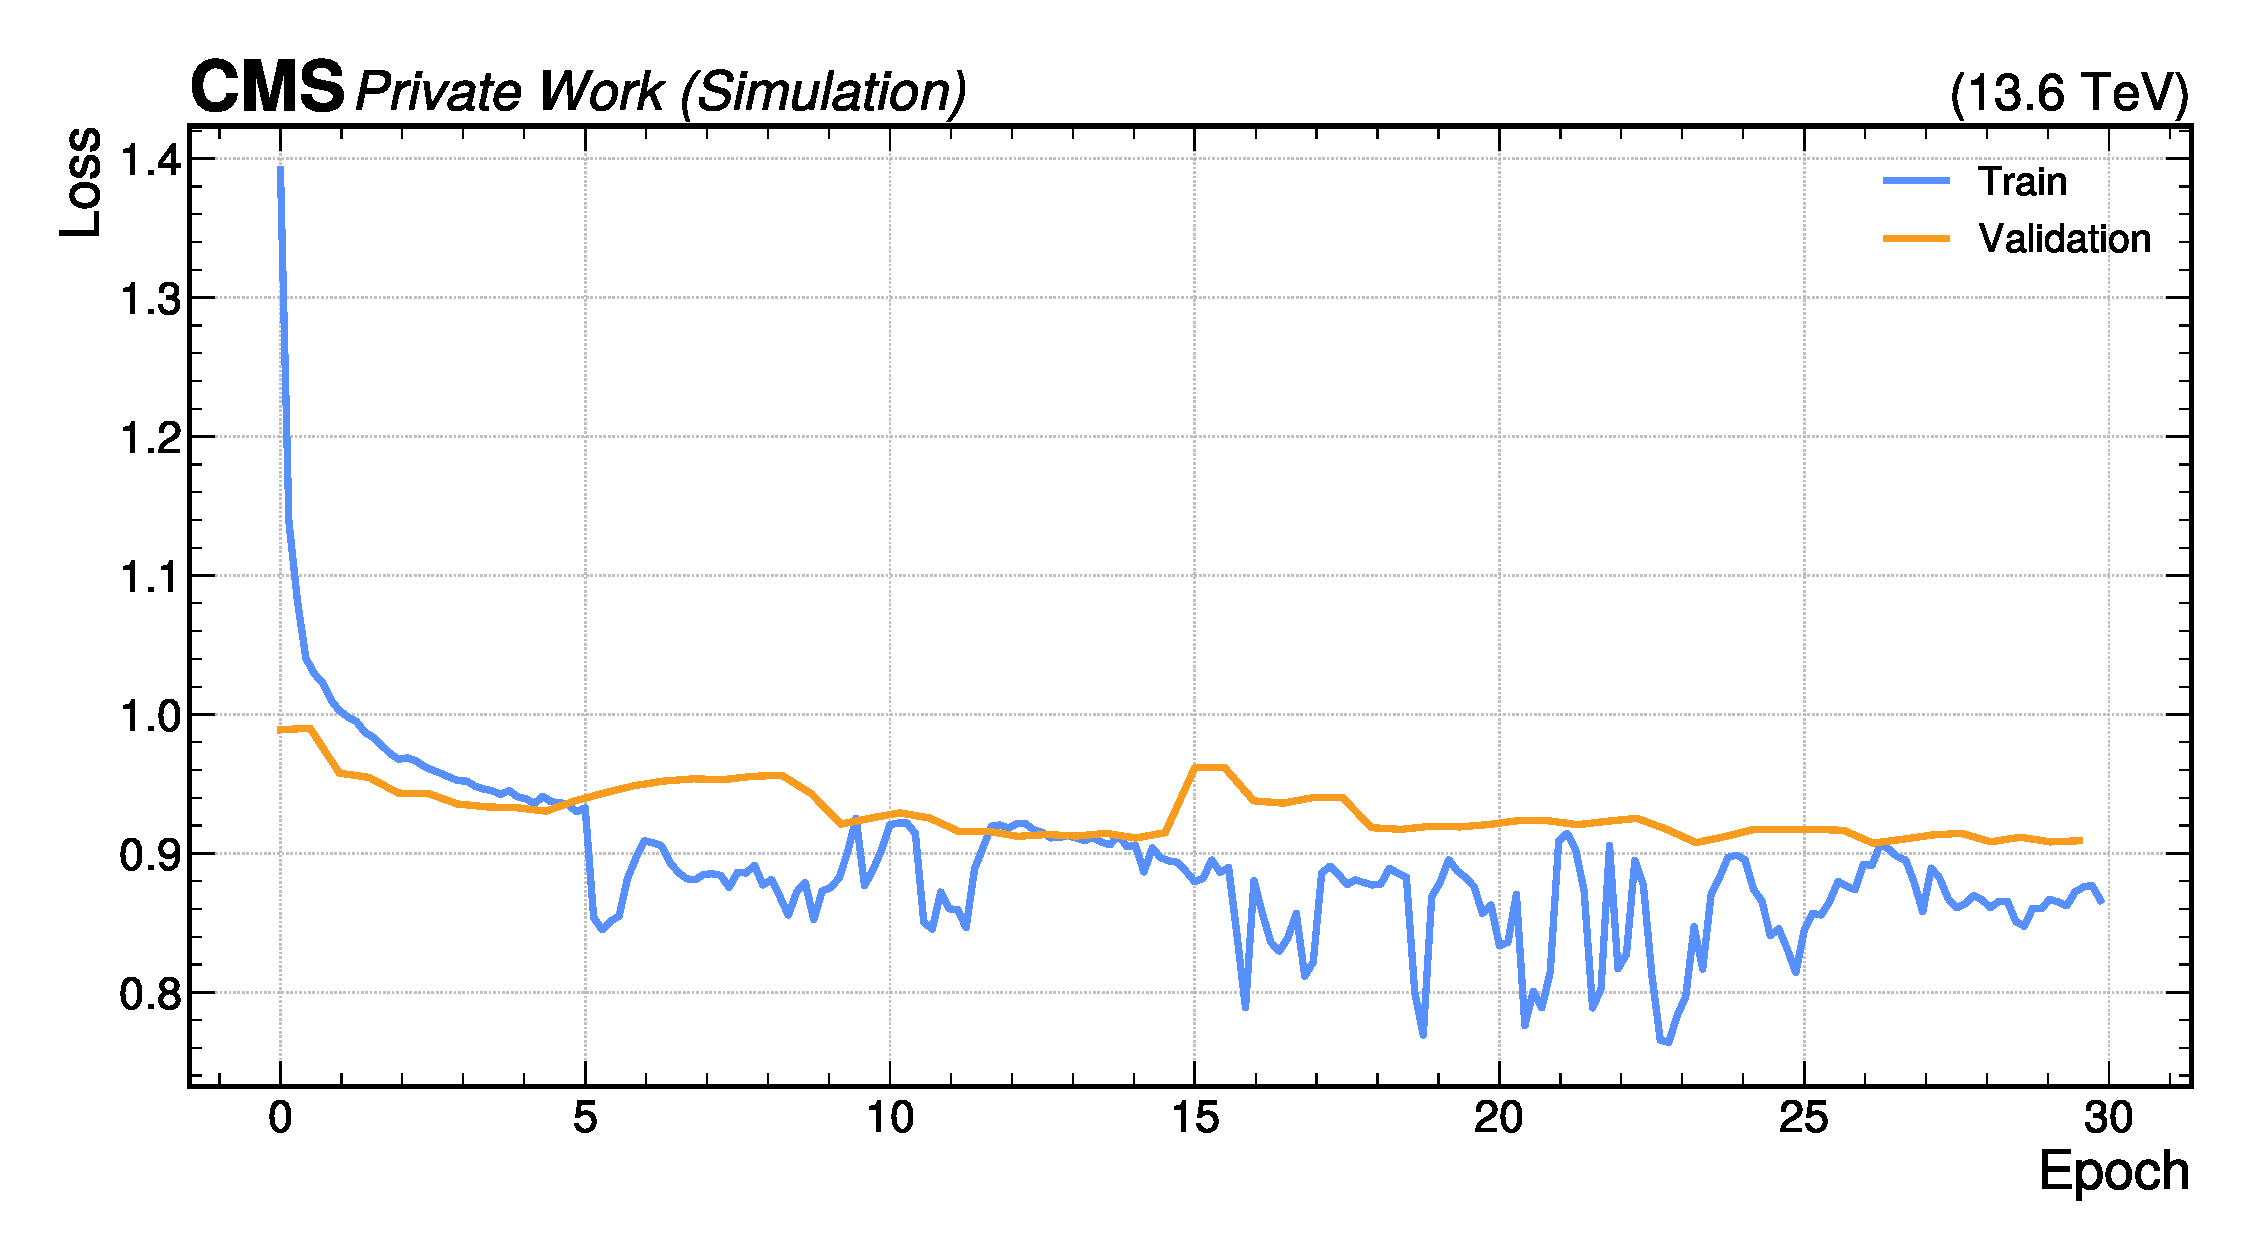
\includegraphics[width=15cm]{media/output/intprob_loss_validation.pdf}
    \caption{Training and validation loss for a PIP trained model over 30 epochs with a sharpness of 1.}
    \label{fig:intprob_training}
\end{figure}

The training loss curve demonstrates visible fluctuations, particularly in comparison to PGD-based training. This instability stems from the discrete nature of PIP perturbations — unlike continuous methods that can produce arbitrarily small perturbations, PIP operates on a finite set of possible integer modifications. This creates less but more pronounced perturbations offering a greater challenge in the training procedure. This instability reflects in the validation loss too, indicating problems to generalize for unseen PIP perturbations. 

Compared to nominal training or PGD, the validation loss slightly exceeds the training loss, suggesting mild adaptation to the lower-severity PIP perturbations \ref{fig:intprob_rocs_training}).

Figure \ref{fig:intprob_rocs_training} shows that the PIP-trained model achieves robust performance against PIP-perturbed data, with an AUC of $0.967$, slightly surpassing the nominal-trained baseline ($AUC = 0.965$) by approximately $0.2\%$. When evaluated on nominal data, the model maintains a strong AUC of $0.962$, indicating minimal performance degradation compared to the undisturbed model.

\begin{figure}[h]
\centering
    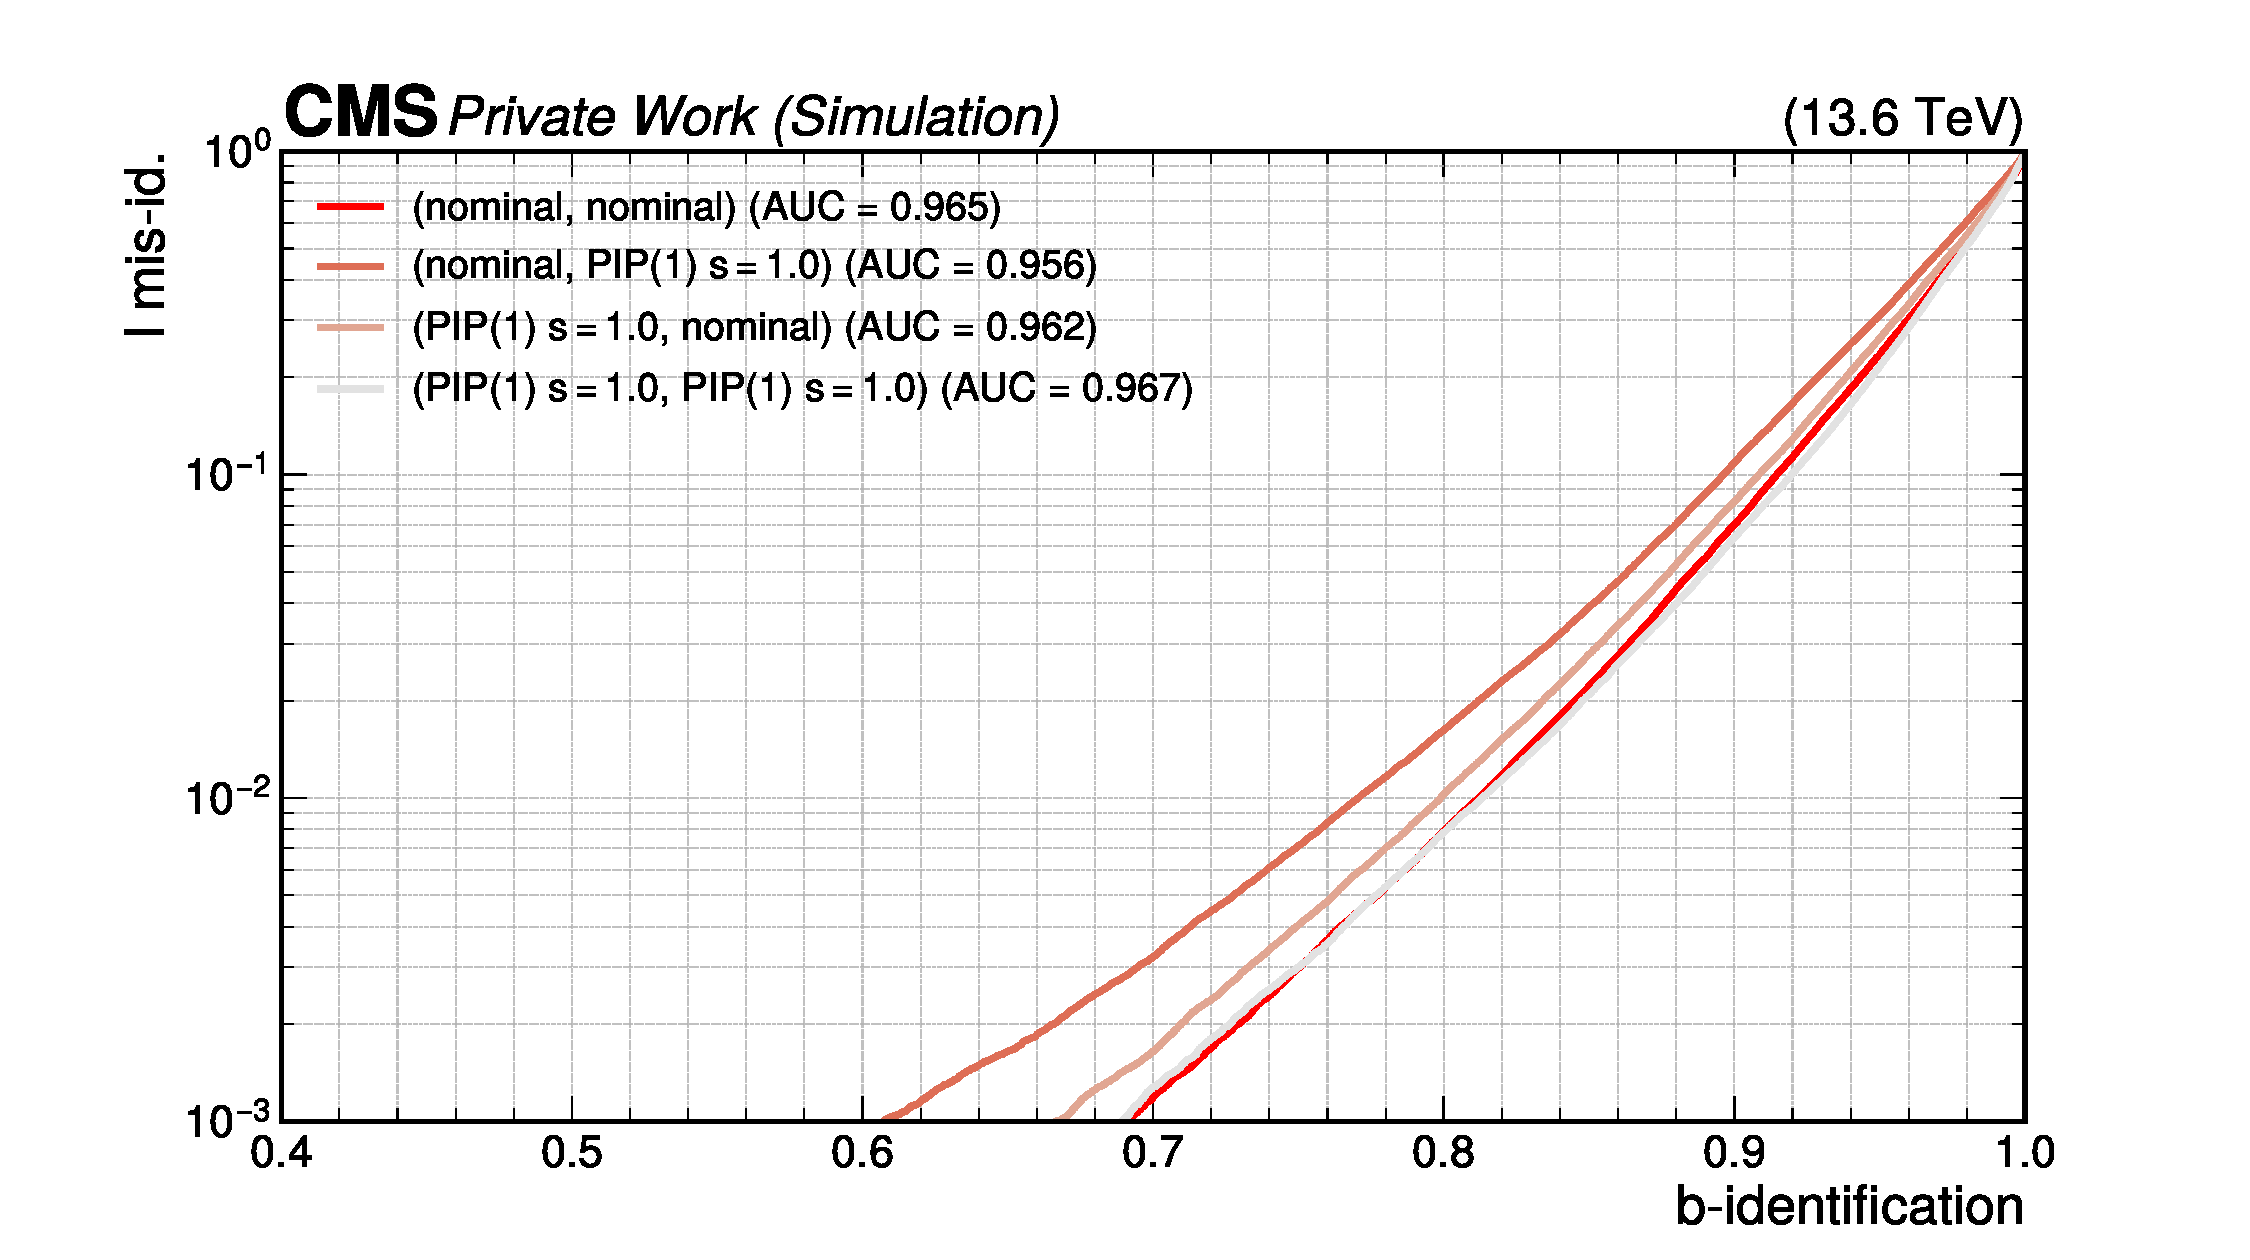
\includegraphics[width=15cm]{media/output/roc_bvsl_intprob_permutations.pdf}
    \caption{ROC curves for BvsL misidentification for a PIP(1) and nominal trained model tested against nominal or PIP(1) perturbed inputs with a sharpness of $s=1.0$.}
    \label{fig:intprob_rocs_training}
\end{figure}

\FloatBarrier
% Joint Application of PIP and PGD
\section{Probabilistic Integer-Perturbed Projected Gradient Descent}

As described in Sec.~\ref{sec:method_combined}, the PIP-PGD attack perturbs floating-point and integer features independently in a single pass. The following analysis examines its effect on input similarity, model performance, and training behaviour.

\paragraph{Severity:} The JSD analysis reveals that combined attacks retain stealth characteristics comparable to standalone PIP or PGD attacks, with JSD values ranging from $\mathcal{O}(10^{-3})$ to $\mathcal{O}(10^{-1})$ across the entire attack domain. A detailed list of JSD values for individual features is provided in Appendix \ref{appendix:combined}.

The histograms between one and two iterations for \texttt{jet\_eta} (float) and \texttt{nsv} (integer) is depicted in figures \ref{fig:combined_input_eta} and \ref{fig:combined_input_vtxAss} respectively. These features were specifically chosen to show the perturbation across discrete and continuous inputs. Their respective JSDs lie approximately within the same order of magnitude.

\begin{figure}[htbp]
  \centering
  \begin{subfigure}[t]{0.5\textwidth}
    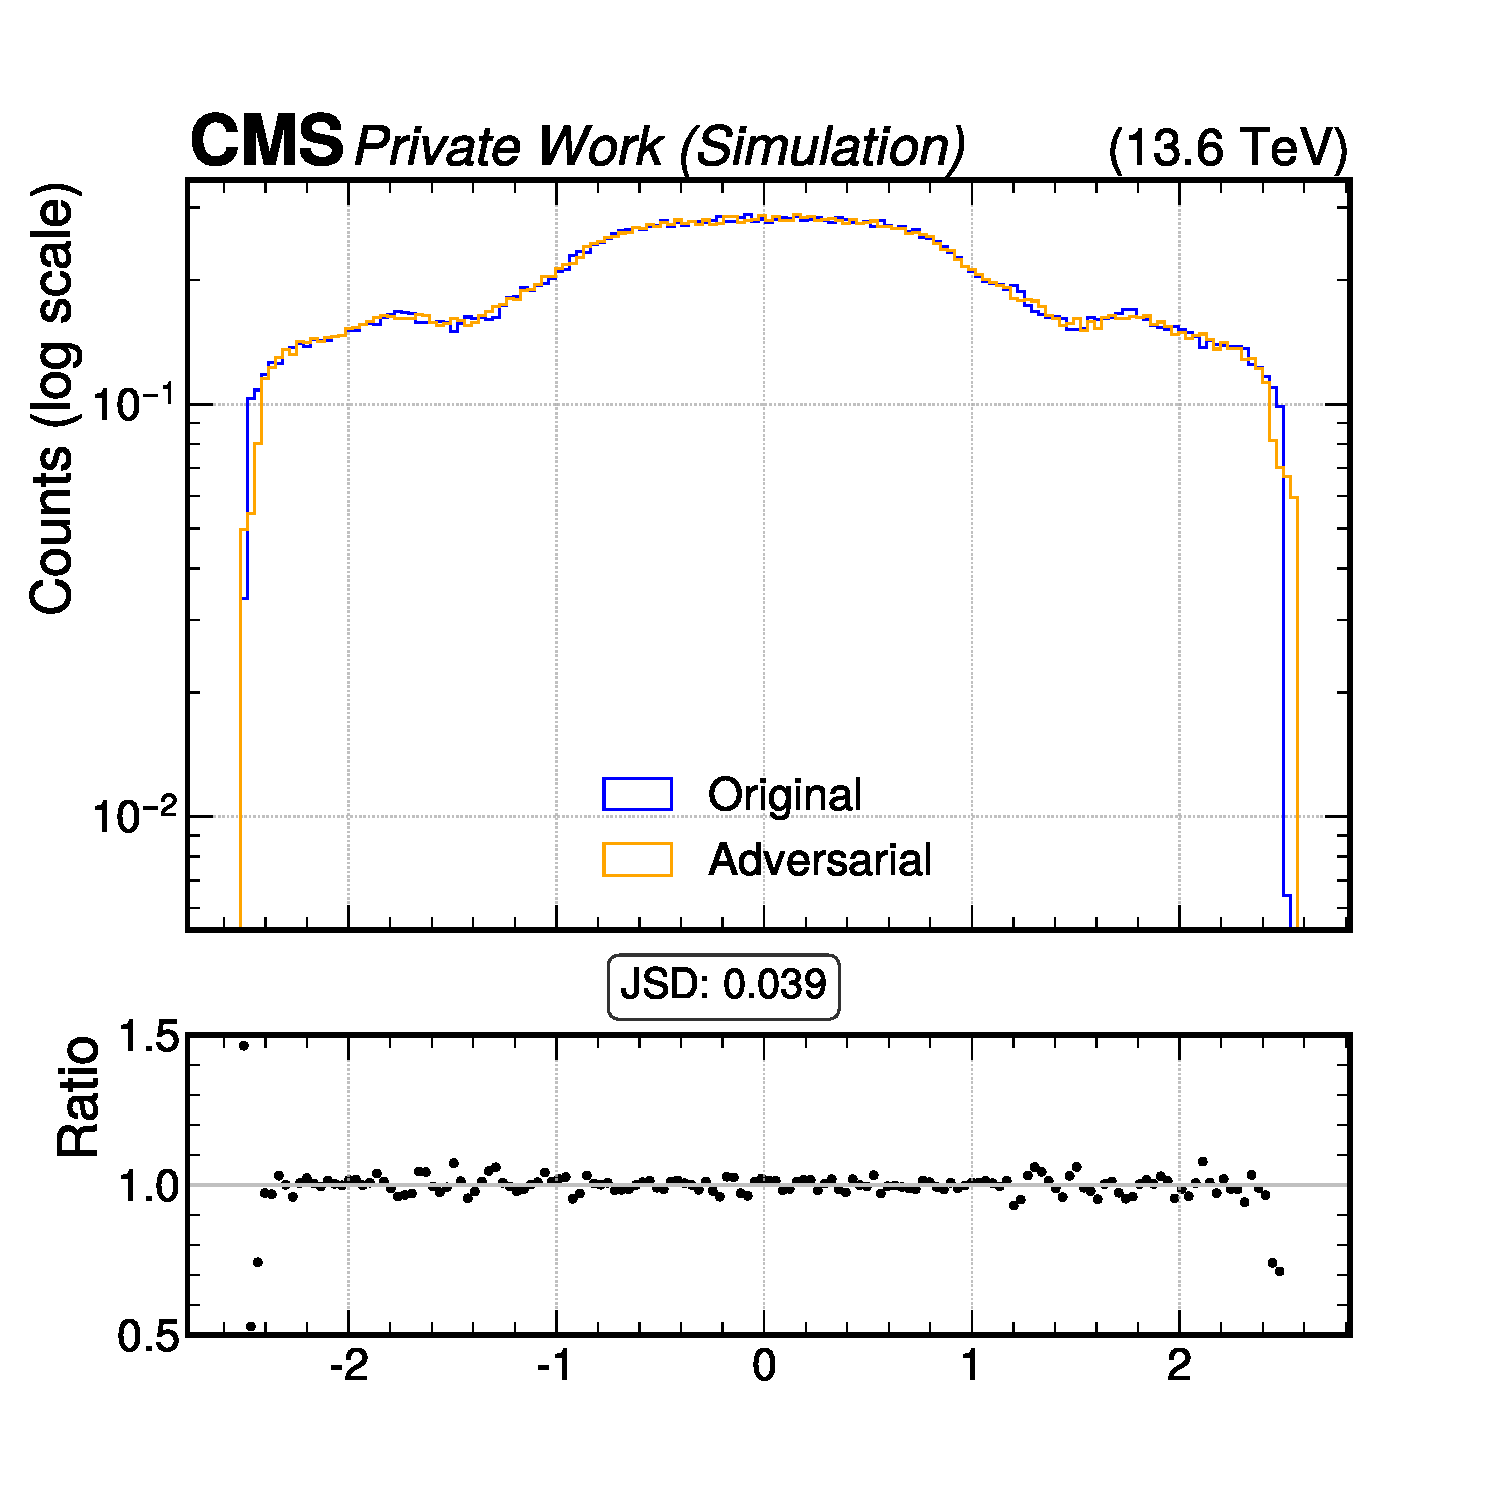
\includegraphics[width=\linewidth]{media/output/features/compare/combined_it_1/cmp_global_features_jet_eta.pdf}
    \caption{Input similarity for PIP-PGD(1).}
    \label{fig:left}
  \end{subfigure}\hfill
  \begin{subfigure}[t]{0.5\textwidth}
    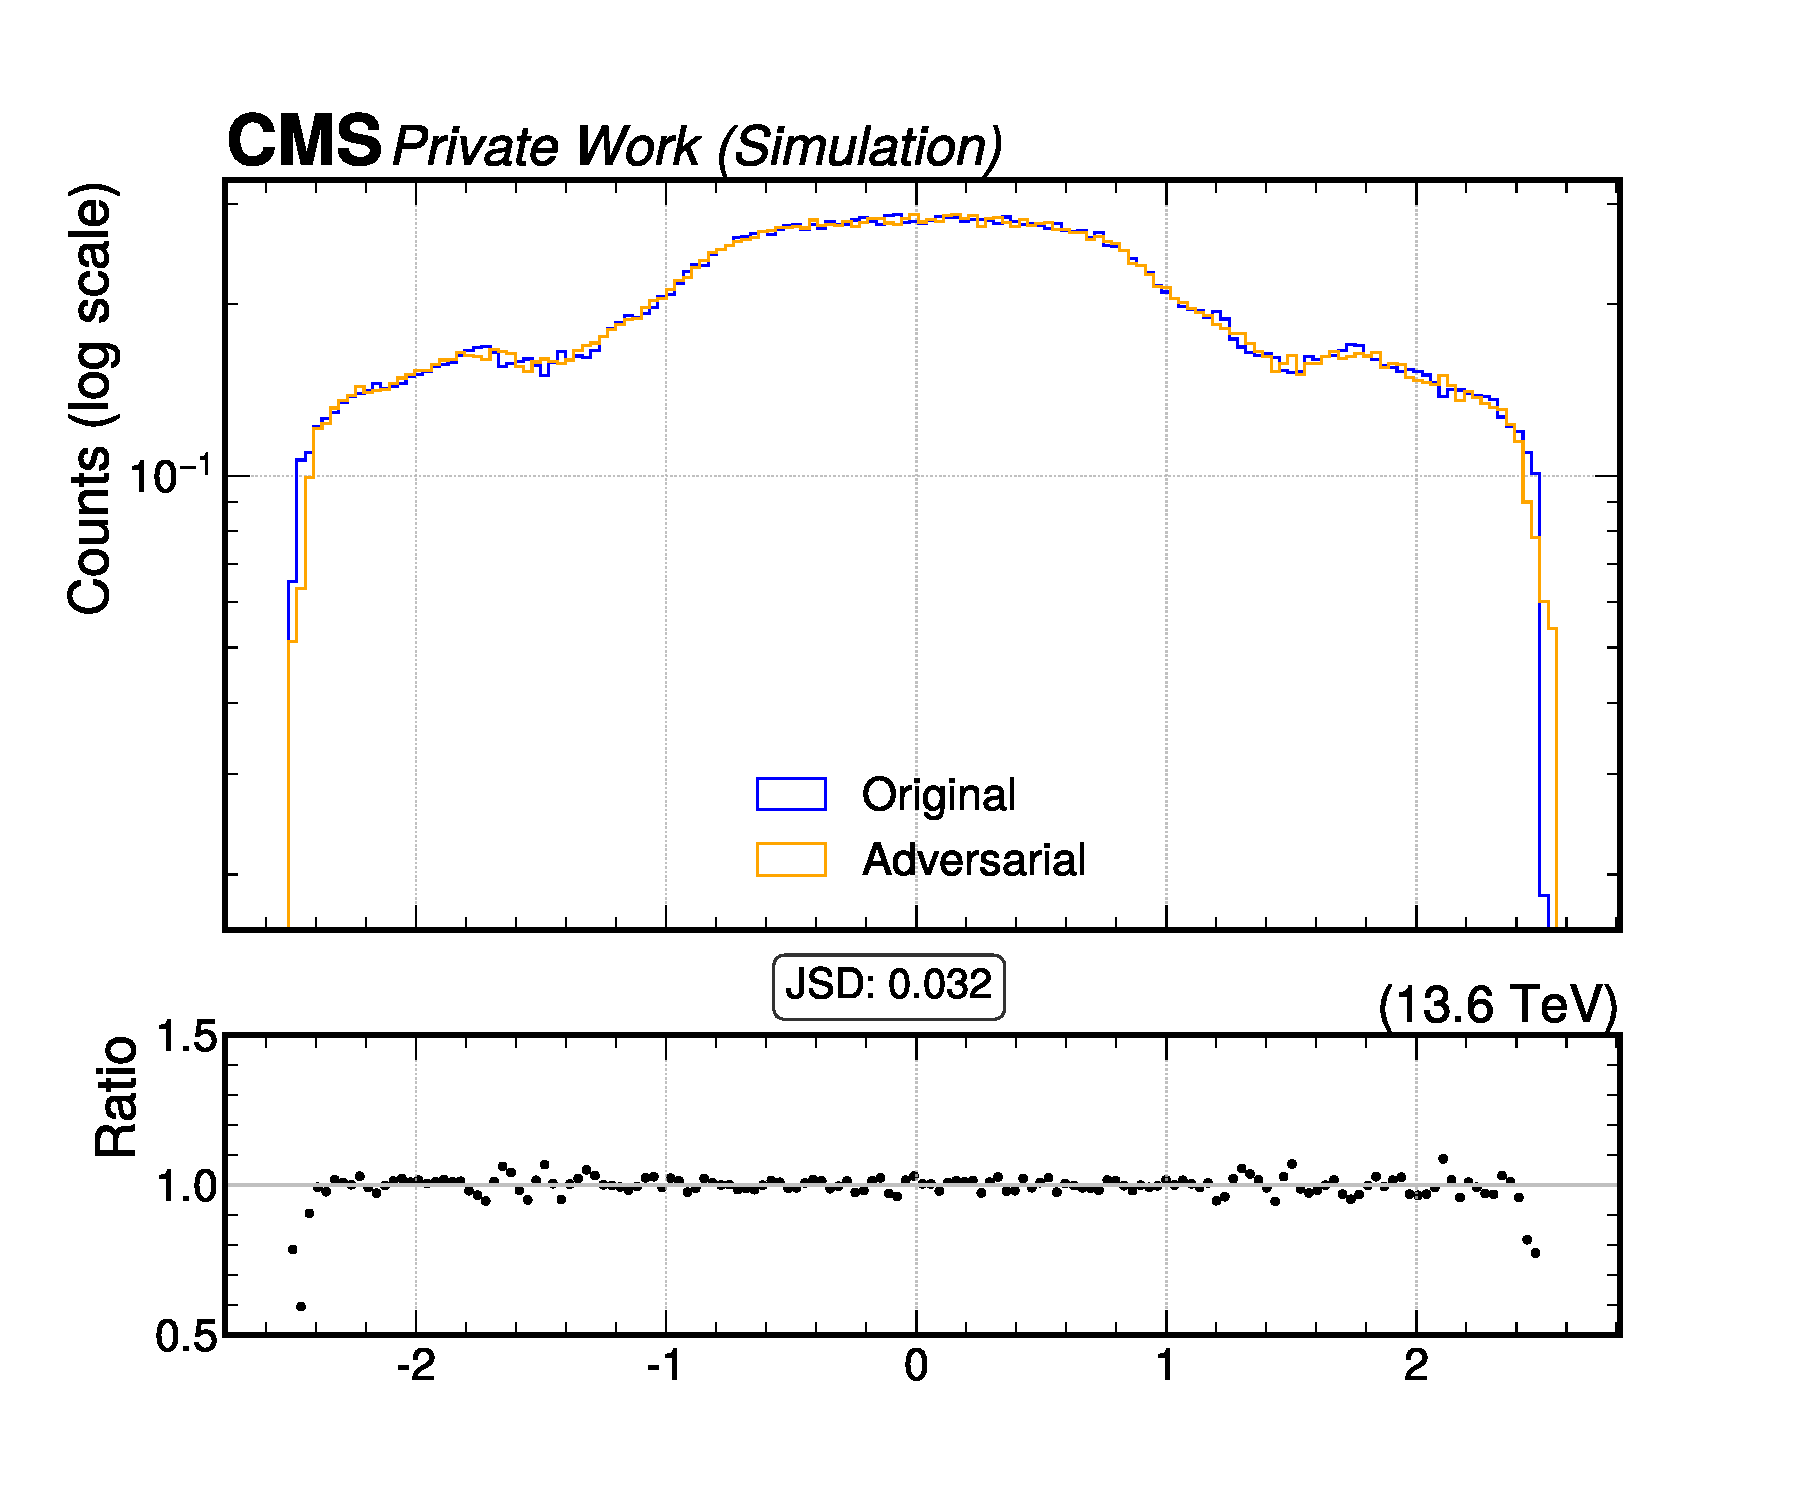
\includegraphics[width=\linewidth]{media/output/features/compare/combined_it_2/cmp_global_features_jet_eta.pdf}
    \caption{Input similarity for PIP-PGD(2).}
    \label{fig:middle}
  \end{subfigure}\hfill

  \caption{Histogram of input perturbation for continuously-valued global \texttt{jet\_eta} for one (left) and two (right) iterations of PIP-PGD compared against nominal inputs.}
  \label{fig:combined_input_eta}
\end{figure}

\begin{figure}[htbp]
  \centering
  \begin{subfigure}[t]{0.5\textwidth}
    \includegraphics[width=\linewidth]{media/output/features/compare/combined_it_1/cmp_global_features_nsv.pdf}
    \caption{Input similarity for PIP-PGD(1).}
    \label{fig:left}
  \end{subfigure}\hfill
  \begin{subfigure}[t]{0.5\textwidth}
    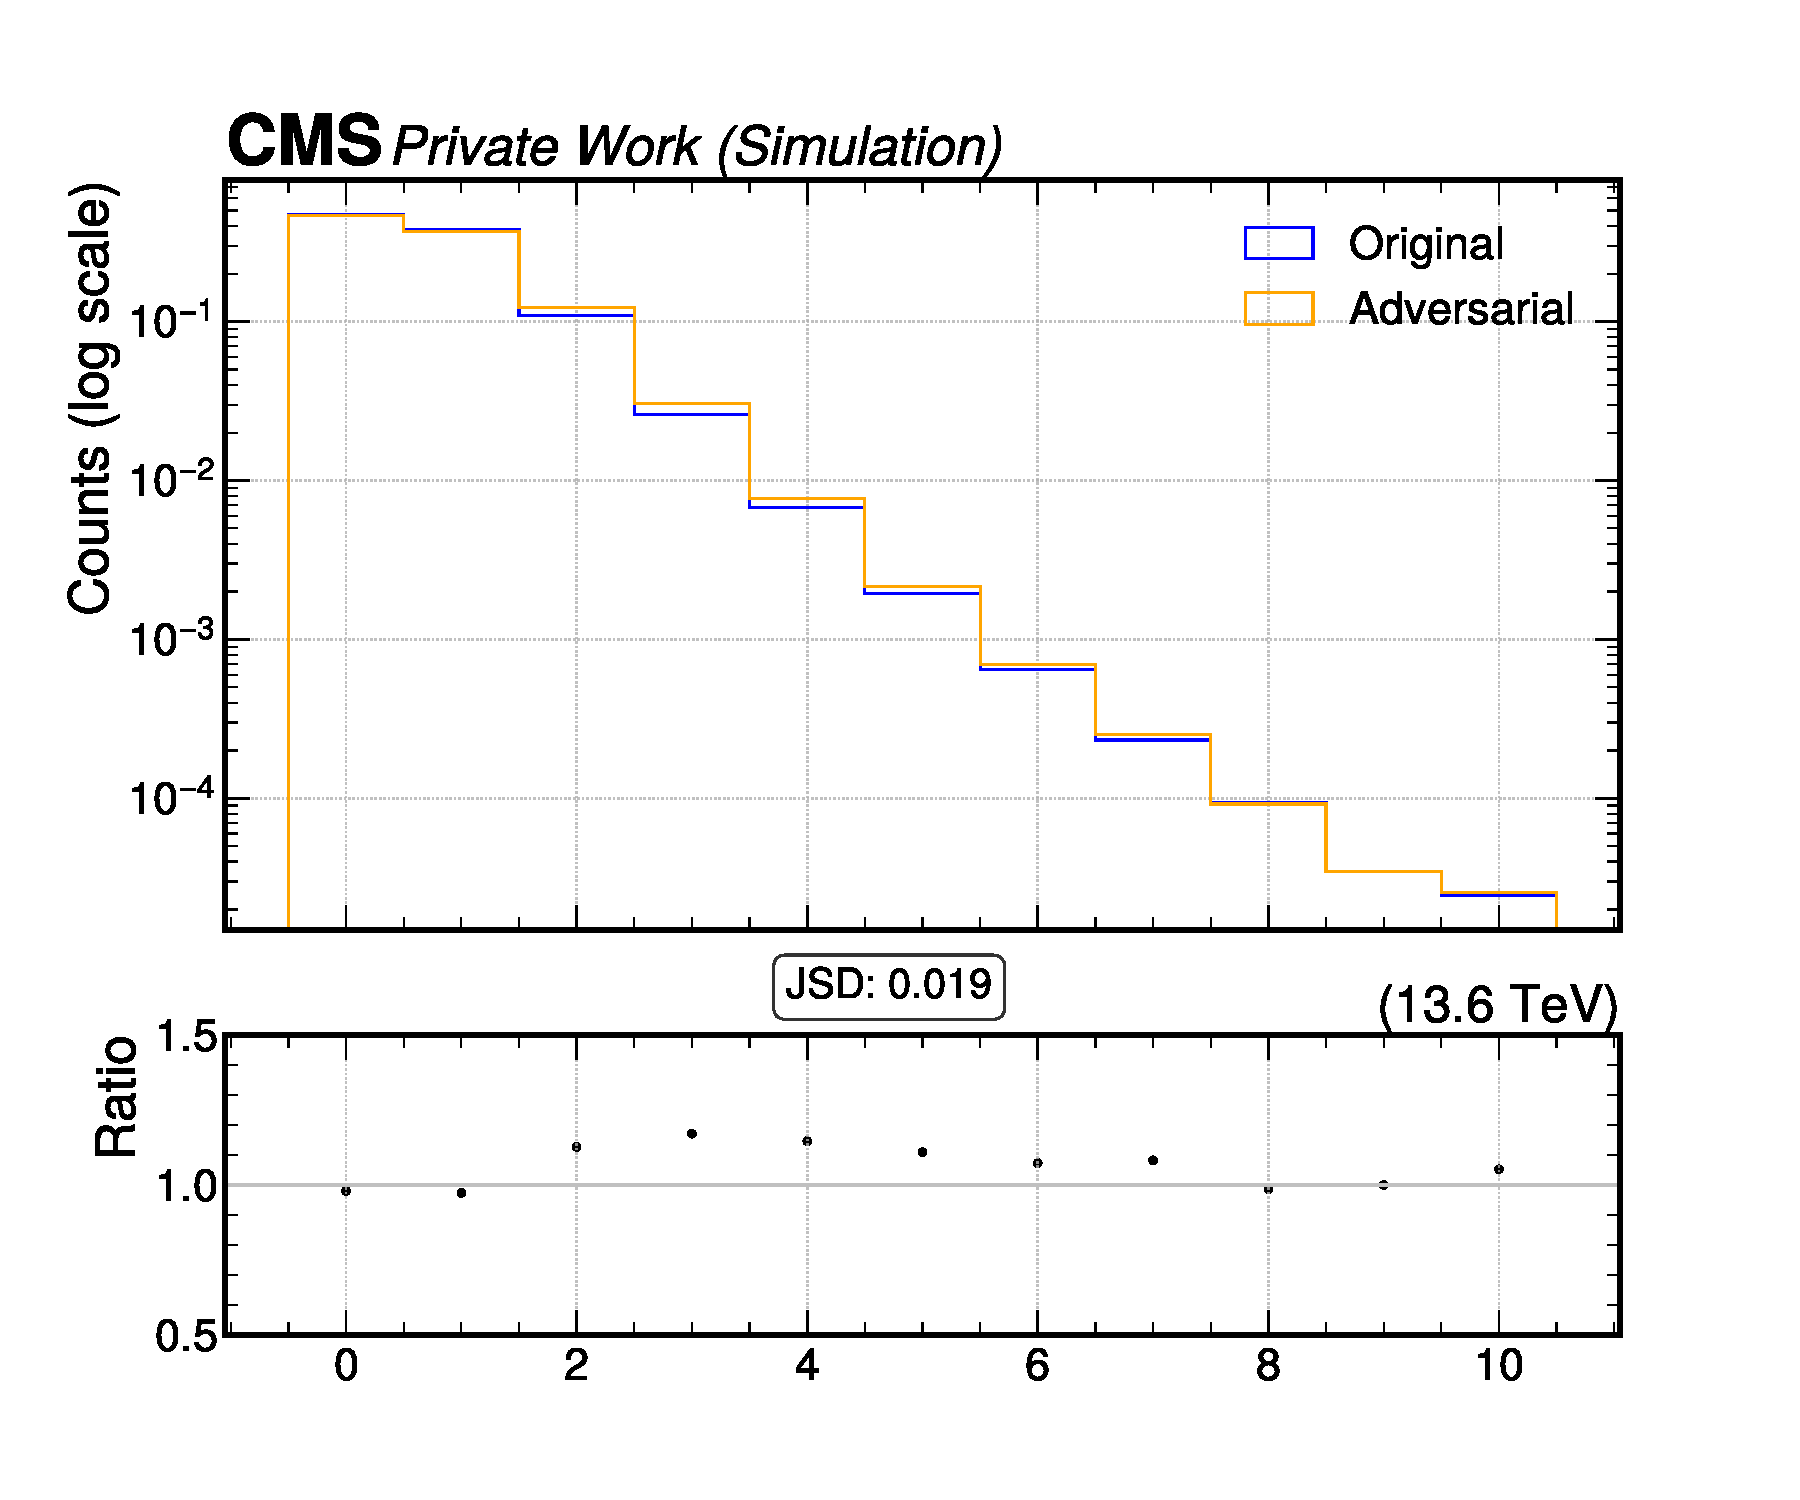
\includegraphics[width=\linewidth]{media/output/features/compare/combined_it_2/cmp_global_features_nsv.pdf}
    \caption{Input similarity for PIP-PGD(2).}
    \label{fig:middle}
  \end{subfigure}\hfill

  \caption{Histogram of input perturbation for discrete-valued global \texttt{nsv} for one (left) and two (right) iterations of PIP-PGD compared against nominal inputs.}
  \label{fig:combined_input_vtxAss}
\end{figure}

Figure \ref{fig:combined_joint_overview} provides an overview of input similarity across all features for the combined PIP-PGD attack, highlighting how different feature types respond to the hybrid perturbation strategy. While certain integer features — which are denoted orange in the figure — such as \\ \texttt{TagVarCSV\_jetNTracksEtaRel}, \texttt{TagVarCSV\_vertexCategory} or \texttt{Cpfcan\_quality} exhibit larger perturbations than others, their overall similarity remains comparable.


\begin{figure}[H]
\centering
    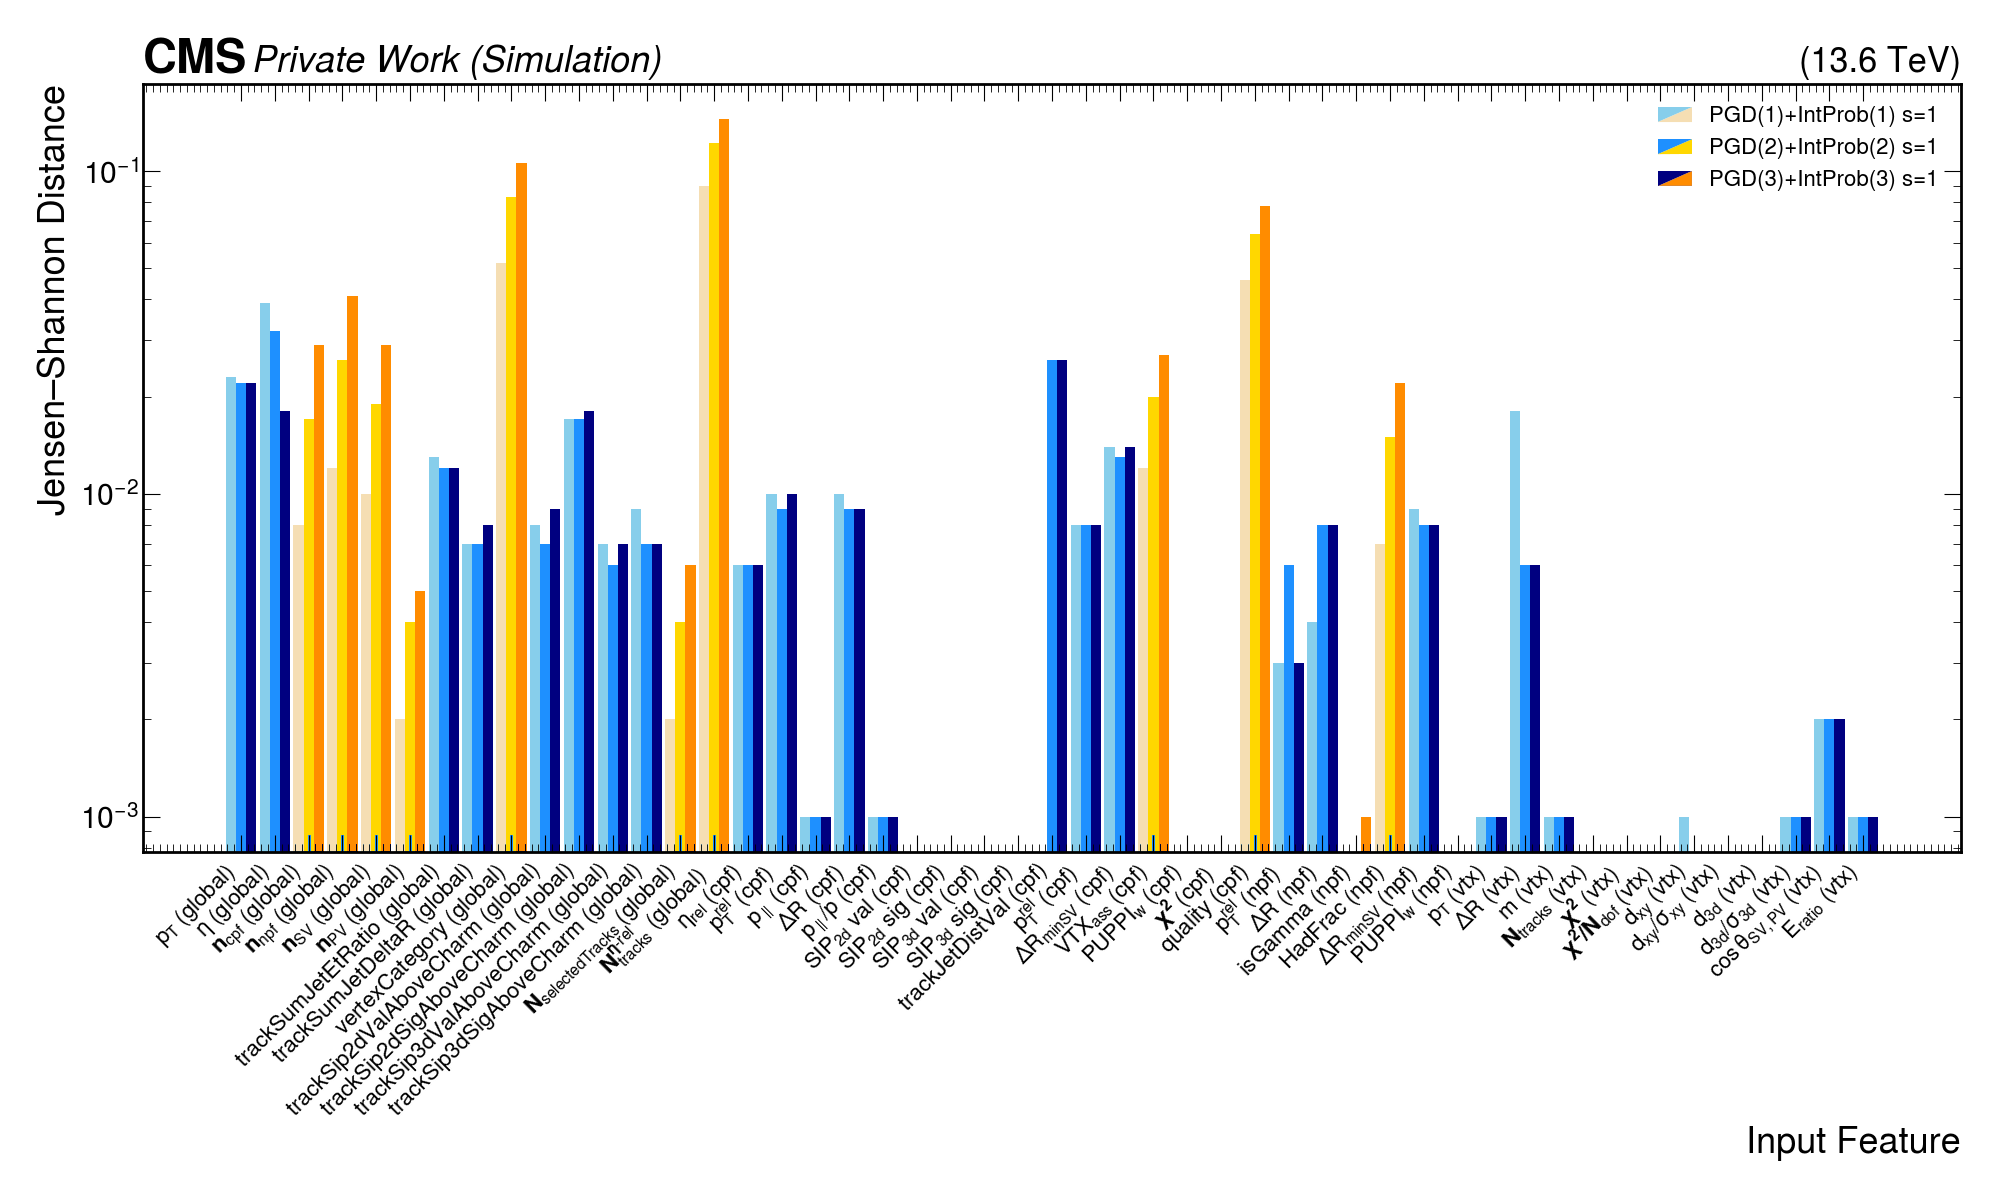
\includegraphics[width=15cm]{media/output/features/compare/jsd_comb_per_feature.pdf}
    \caption{JSD input similarity development for different iterations of the PIP-PGD attack for $s=1$ and $\epsilon=0.1$ while attributing for individual features. Orange bars denote integer based features, blue bars correspond to floating-point features. Values below $10^{-1}$ are not included due to rounding.}
    \label{fig:combined_joint_overview}
\end{figure}

The pattern indicates that the combined attack balances stealth and efficacy effectively: integer features introduce targeted modifications atop continuous feature perturbations, enabling a more aggressive perturbation strategy. 

\paragraph{Attack:} This increased aggression is apparent for variations in the applied sharpness ranging from a slight degradation at $s=5$ ($AUC=0.936$) towards a moderate impact at $s=1$ ($AUC=0.928$) and a severe degradation at $s=0.5$ with an AUC of $0.916$  as seen in figure \ref{fig:combined_testing_sharpness}. The gap between nominal performance ($AUC=0.965$) and PIP at $s=5$ is predominately caused by PGD(1) ($AUC=0.937$, see figure \ref{fig:pgd_trained}).

\begin{figure}[h]
\centering
    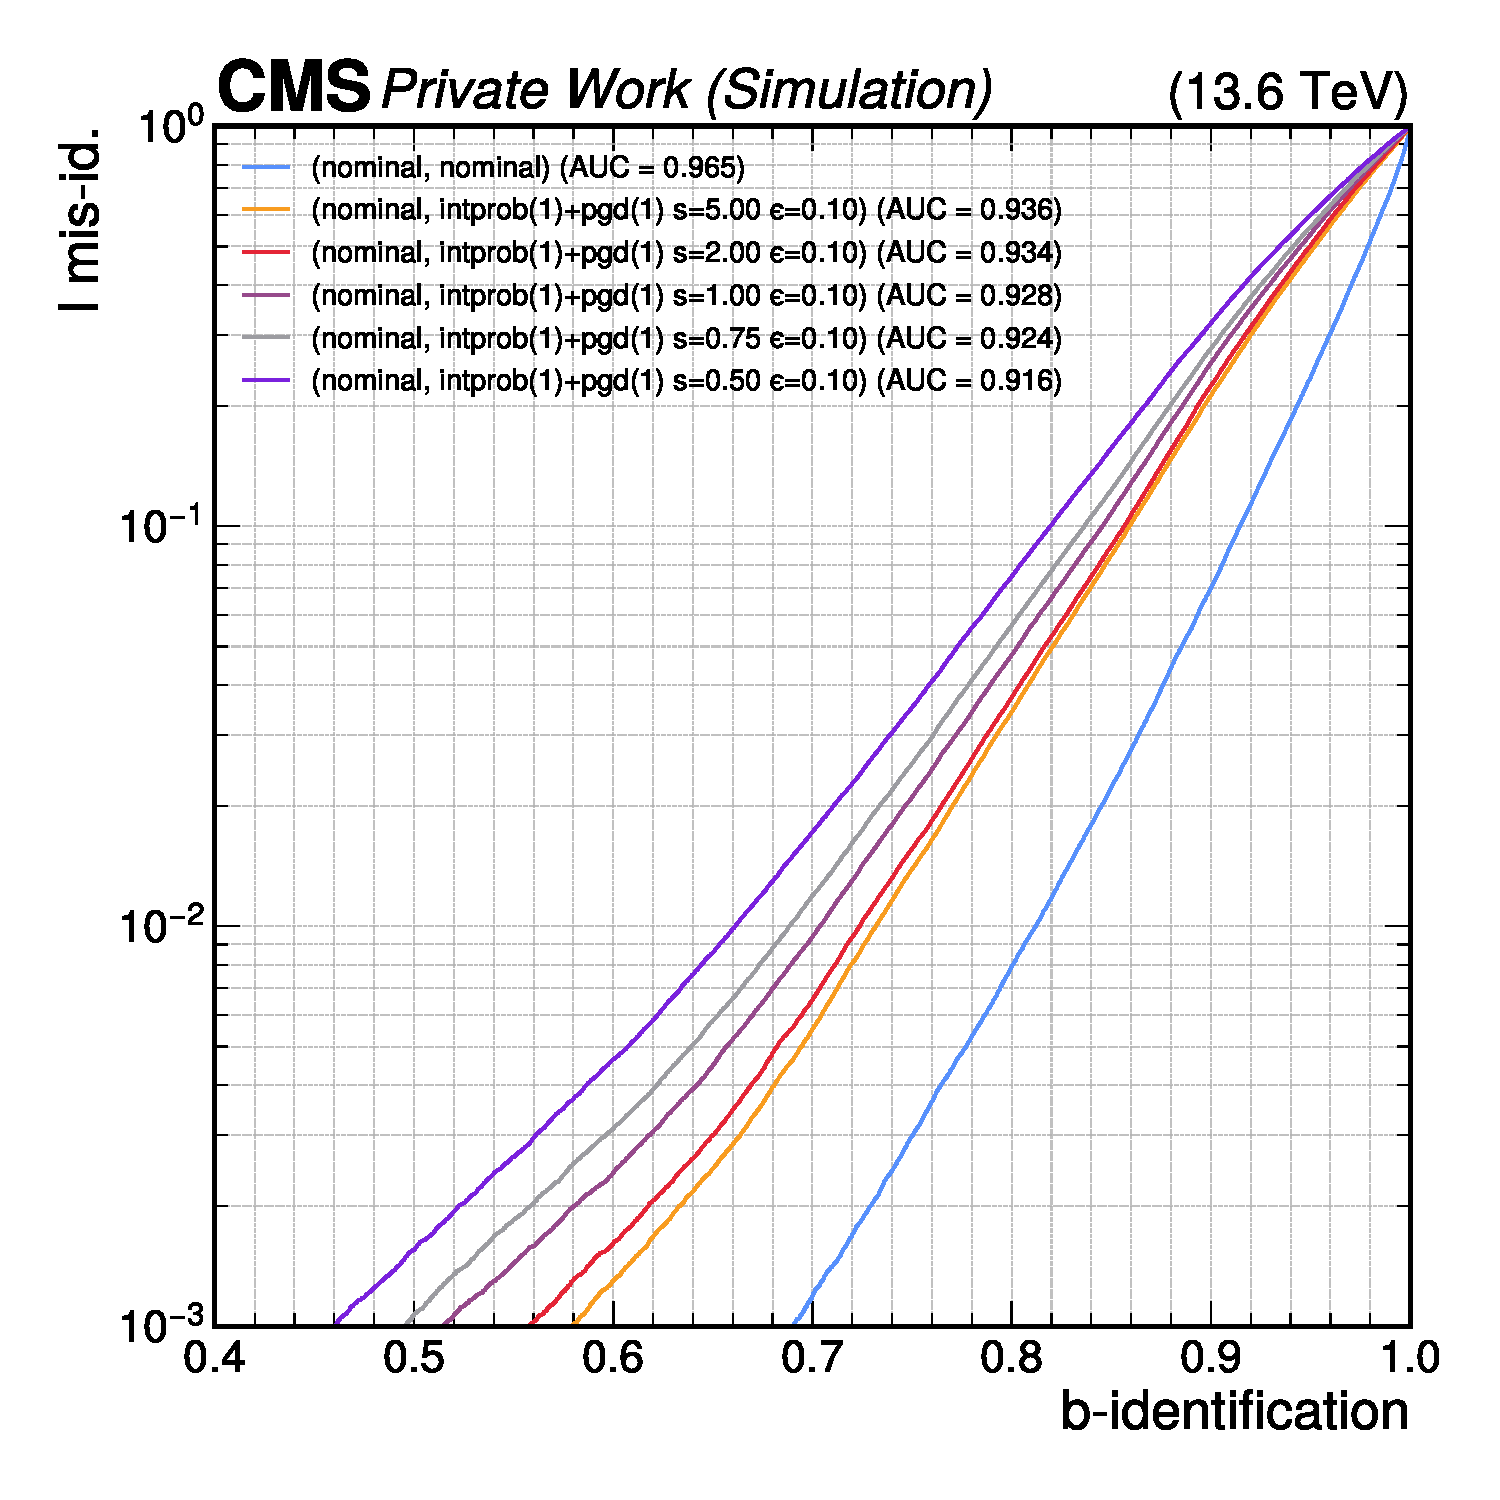
\includegraphics[width=15cm]{media/output/roc_bvsl_combined_sharpness.pdf}
    \caption{AUC score of BvsL misidentification for PIP-PGD with sharpness between $s=0.5$ and $s=5$ at one iteration with a magnitude of $\epsilon=0.10$ tested against the nominal trained model.}
    \label{fig:combined_testing_sharpness}
\end{figure}

Likewise, the AUC score degrades with increasing iterations for the combined PIP-PGD attack from $AUC=0.928$ at one iteration towards stark inference of $AUC=0.885$ at five (see figure \ref{fig:combined_testing_iterations}). The continued AUC decline for iterations > 1 is largely due to PIP stochastic nature, as discussed in Section \ref{sec:inprob_result}.

\begin{figure}[h]
\centering
    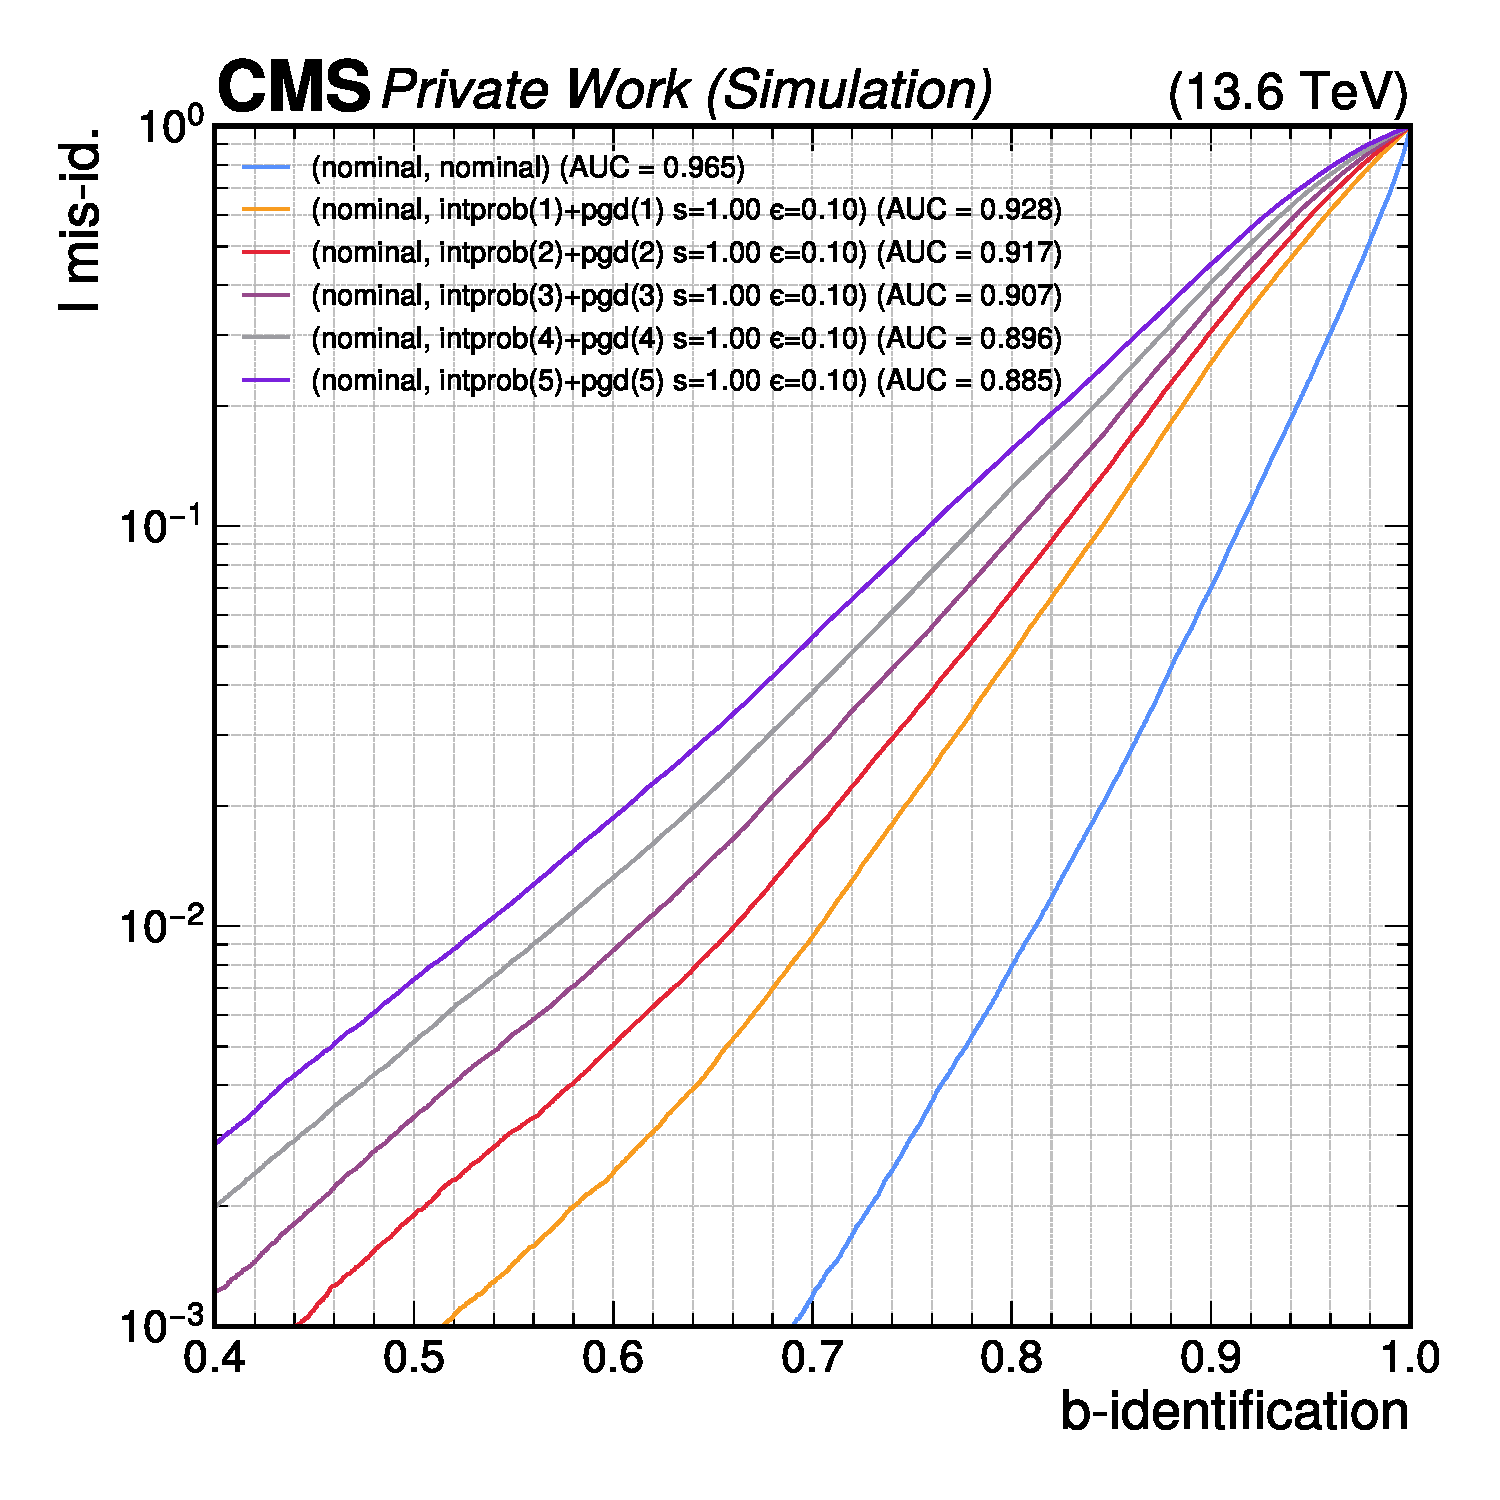
\includegraphics[width=15cm]{media/output/roc_bvsl_combined_iterations.pdf}
    \caption{AUC score of PIP-PGD for BvsL misidentification for up to 5 iterations with a fixed magnitude of $\epsilon=0.1$ and a sharpness of $s=1$ tested against the nominal trained model.}
    \label{fig:combined_testing_iterations}
\end{figure}


\begin{figure}[H]
\centering
    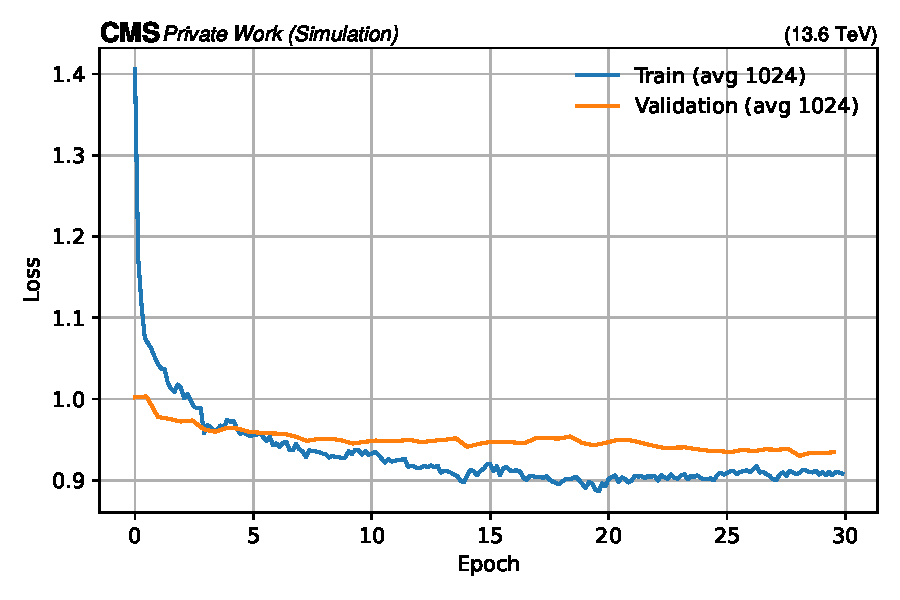
\includegraphics[width=15cm]{media/output/combined_loss_validation.pdf}
    \caption{Training and validation loss for PIP-PGD(1) with a sharpness of $s=1$ and a magnitude of $\epsilon=0.1$, while scaling individual attack features based on an epsilon tensor.}
    \label{fig:combined_training_loss}
\end{figure}


\FloatBarrier
\paragraph{Adversarial Training:} The training loss curve (see figure \ref{fig:combined_training_loss}) for PIP-PGD exhibits moderate volatility, falling between the stability of pure PGD training and the higher volatility of PIP training . This intermediate behaviour is attributable to the model's need to develop defences that are effective against continuous and probabilistic discrete modifications.



The validation loss demonstrates robust generalization, suggesting that the combined training approach successfully teaches the model to recognize and resist both perturbation types. The convergence pattern indicates that the model learns to balance the competing objectives of maintaining nominal performance while developing comprehensive adversarial defences.

Notably, the final validation loss values are competitive with single-method adversarial training and even surpass pure PIP training. This is an indication that the combined approach does not sacrifice overall performance for broader robustness. It furthermore suggests that the two perturbation types target complementary aspects of the model's decision boundaries, allowing for more comprehensive defence development.

The training efficiency appears reasonable, with convergence achieved within a similar time frame to single-method approaches. This efficiency is particularly important given the increased computational complexity of generating both types of adversarial examples during training.

\begin{figure}[h]
\centering
    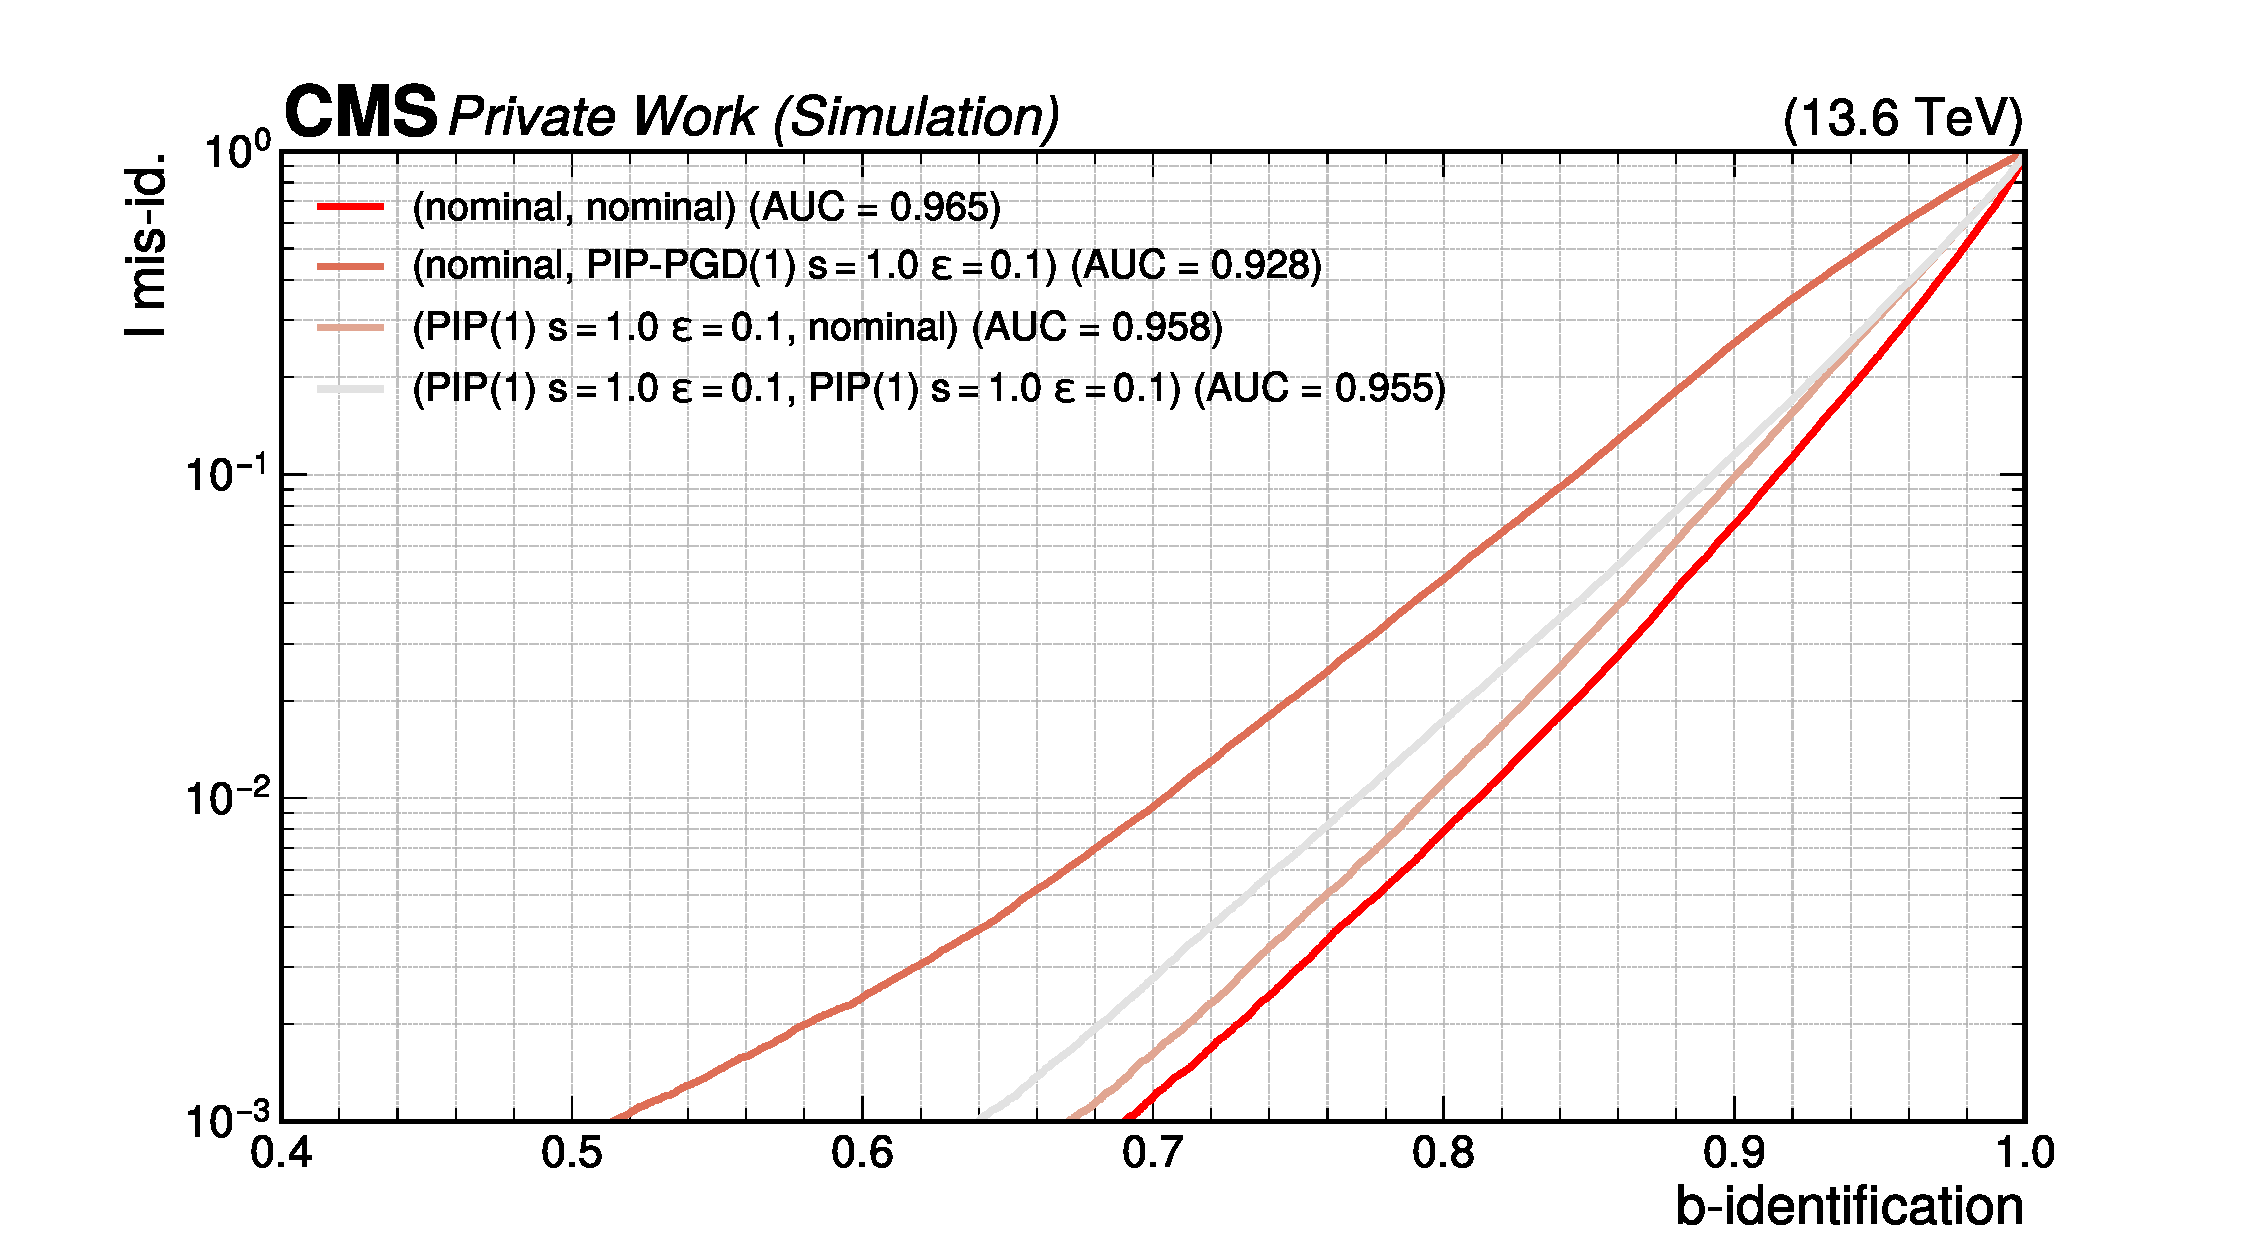
\includegraphics[width=15cm]{media/output/roc_bvsl_combined_crossing.pdf}
    \caption{ROC curves for BvsL misidentification for a PIP-PGD(1) and nominal trained model tested against nominal or PIP-PGD(1) perturbed inputs with $s=1.0$ and $\epsilon=0.1$.}
    \label{fig:joint_training_crossing}
\end{figure}

Figure \ref{fig:joint_training_crossing} shows that the adversarially trained PIP-PGD model, with an AUC of $0.958$ against nominal inputs, closely matches the baseline AUC for nominal inputs ($AUC = 0.965$). It also demonstrates robustness across PGD ($AUC = 0.952$), PIP ($AUC = 0.960$), and itself ($AUC = 0.955$). Compared to the nominal-trained model on PIP-PGD perturbed data ($AUC = 0.928$), the PIP-PGD model achieves consistently strong performance across all tested scenarios.




\FloatBarrier
\section{Transferability and Cross-Robustness}

This section concludes the evaluation of PIP by assessing the transferability and cross-robustness of adversarial training strategies, with a focus on the combined PIP-PGD attack. By analysing the interplay of \textit{iteration count} and \textit{sharpness} in PIP’s variability and assessing robustness across diverse attack scenarios, it is demonstrated how the hybrid approach balances efficacy and generalization.

\subsection{Variability of PIP}
\label{sec:intprob_variability}

\begin{figure}[h]
\centering
    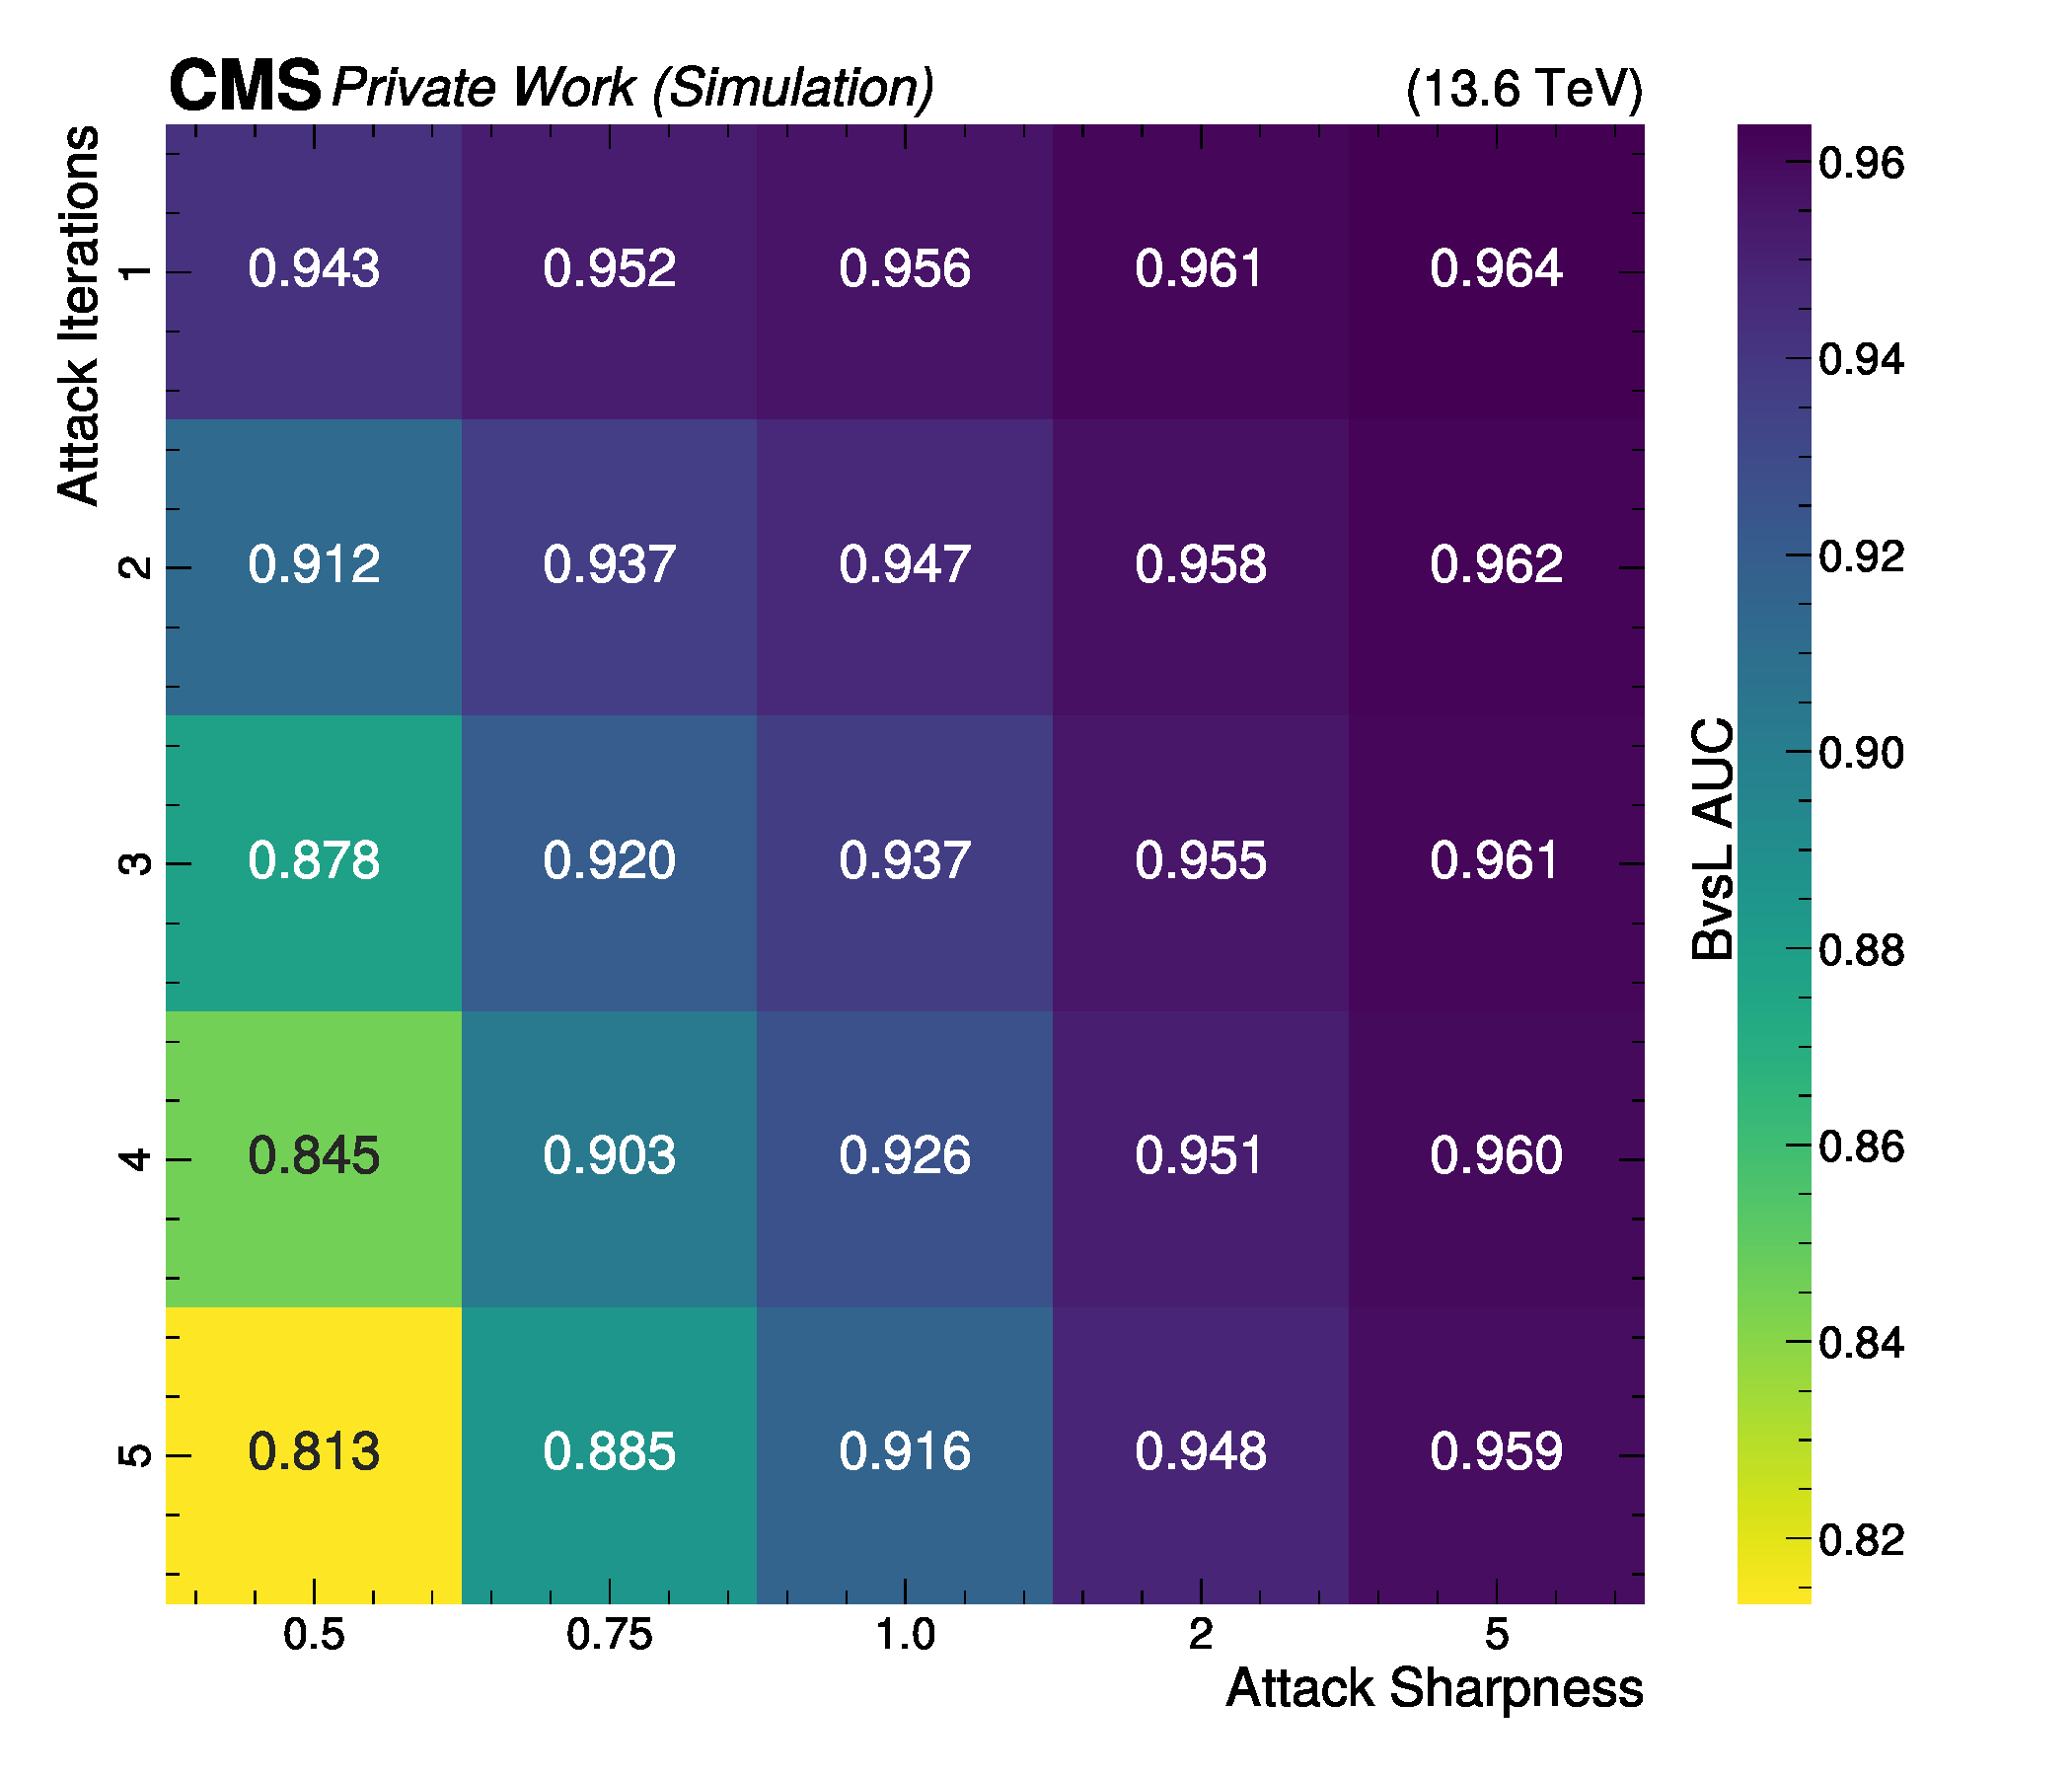
\includegraphics[width=15cm]{media/output/sharpness_iterations_scan.pdf}
    \caption{AUC score matrix of BvsL misidentification for different iteration and sharpness values in the PIP-PGD attack tested against the nominal trained model.}
    \label{fig:joint_sharpness_vs_iterarions}
\end{figure}

Figure~\ref{fig:joint_sharpness_vs_iterarions} visualises the impact of jointly varying the \emph{iteration count} $k$ (rows) and the \emph{sharpness} parameter $s$ (columns) on the attack efficacy for PIP. For each $(k,s)$ point the resulting BvsL AUC is reported after the attack has been applied to the nominally trained model. Notably, the heatmap is inverted to emphasize stronger degradation from the nominal baseline.

\newpage
\paragraph{Key trends.}
\begin{enumerate}
  \item \textbf{Iteration depth controls raw attack power.}  
        Increasing from $k=1$ (single-step FGSM/PIP) to $k=5$ the AUC degrades monotonically, with the most pronounced drop occurring for low-$s$ columns.  Concretely, the AUC falls from $0.943$ to $0.813$ at
        $(s{=}0.5)$ — a relative reduction of roughly 13\% for only four extra gradient evaluations.
  \item \textbf{Sharpness $s$ trades off focus against coverage.}
        As anticipated in section \ref{sec:intprob_methodology}, large $s$ produces a more sparse integer perturbation pattern, meaning the attack relies mainly on the continuous PGD component. This yields noticeably smaller AUC drops (right-most column remains ${\gtrsim}0.959$ even at $k{=}5$).
        Conversely, $s\!\le\!1$ flips a broader set of integer features; the
        attack strength then scales almost linearly with $k$.
  \item \textbf{Region for practical settings.}  
        The contour where $\text{AUC}\!\approx\!0.937$ — the same degradation as for PGD(1) — occurs at $(k{=}3,\,s{=}1)$. Any application of a combined attack should therefore lie below this threshold (so at higher sharpness or less iterations) to not overshadow the application of PGD(1).
\end{enumerate}

The heatmap highlights the flexibility of PIP: by adjusting iteration count $k$ and sharpness $s$, one can interpolate between subtle, nearly imperceptible perturbations and aggressive attacks that reduce the tagger’s performance by $\gtrsim15\%$, targeting only integer features. The $(k,s)$ plane is non-degenerate, with no single optimal setting; the ideal configuration depends on prioritizing stealth (larger $s$, smaller $k$) or maximum performance degradation (smaller $s$, larger $k$). Thus, PIP can be tuned to remain subtle when combined with other attacks while enhancing robustness against integer-based corruption, extending existing adversarial algorithms.

\subsection{Cross-Robustness of PIP-PGD}

The last section of this thesis focuses on a cross-robustness study between trained and tested models across all previous mentioned adversarial attacks. For the sake of simplicity, a sharpness of $s=1$, PGD magnitude of $\epsilon=0.1$, and only one iteration is discussed here.

\begin{figure}[h]
\centering
    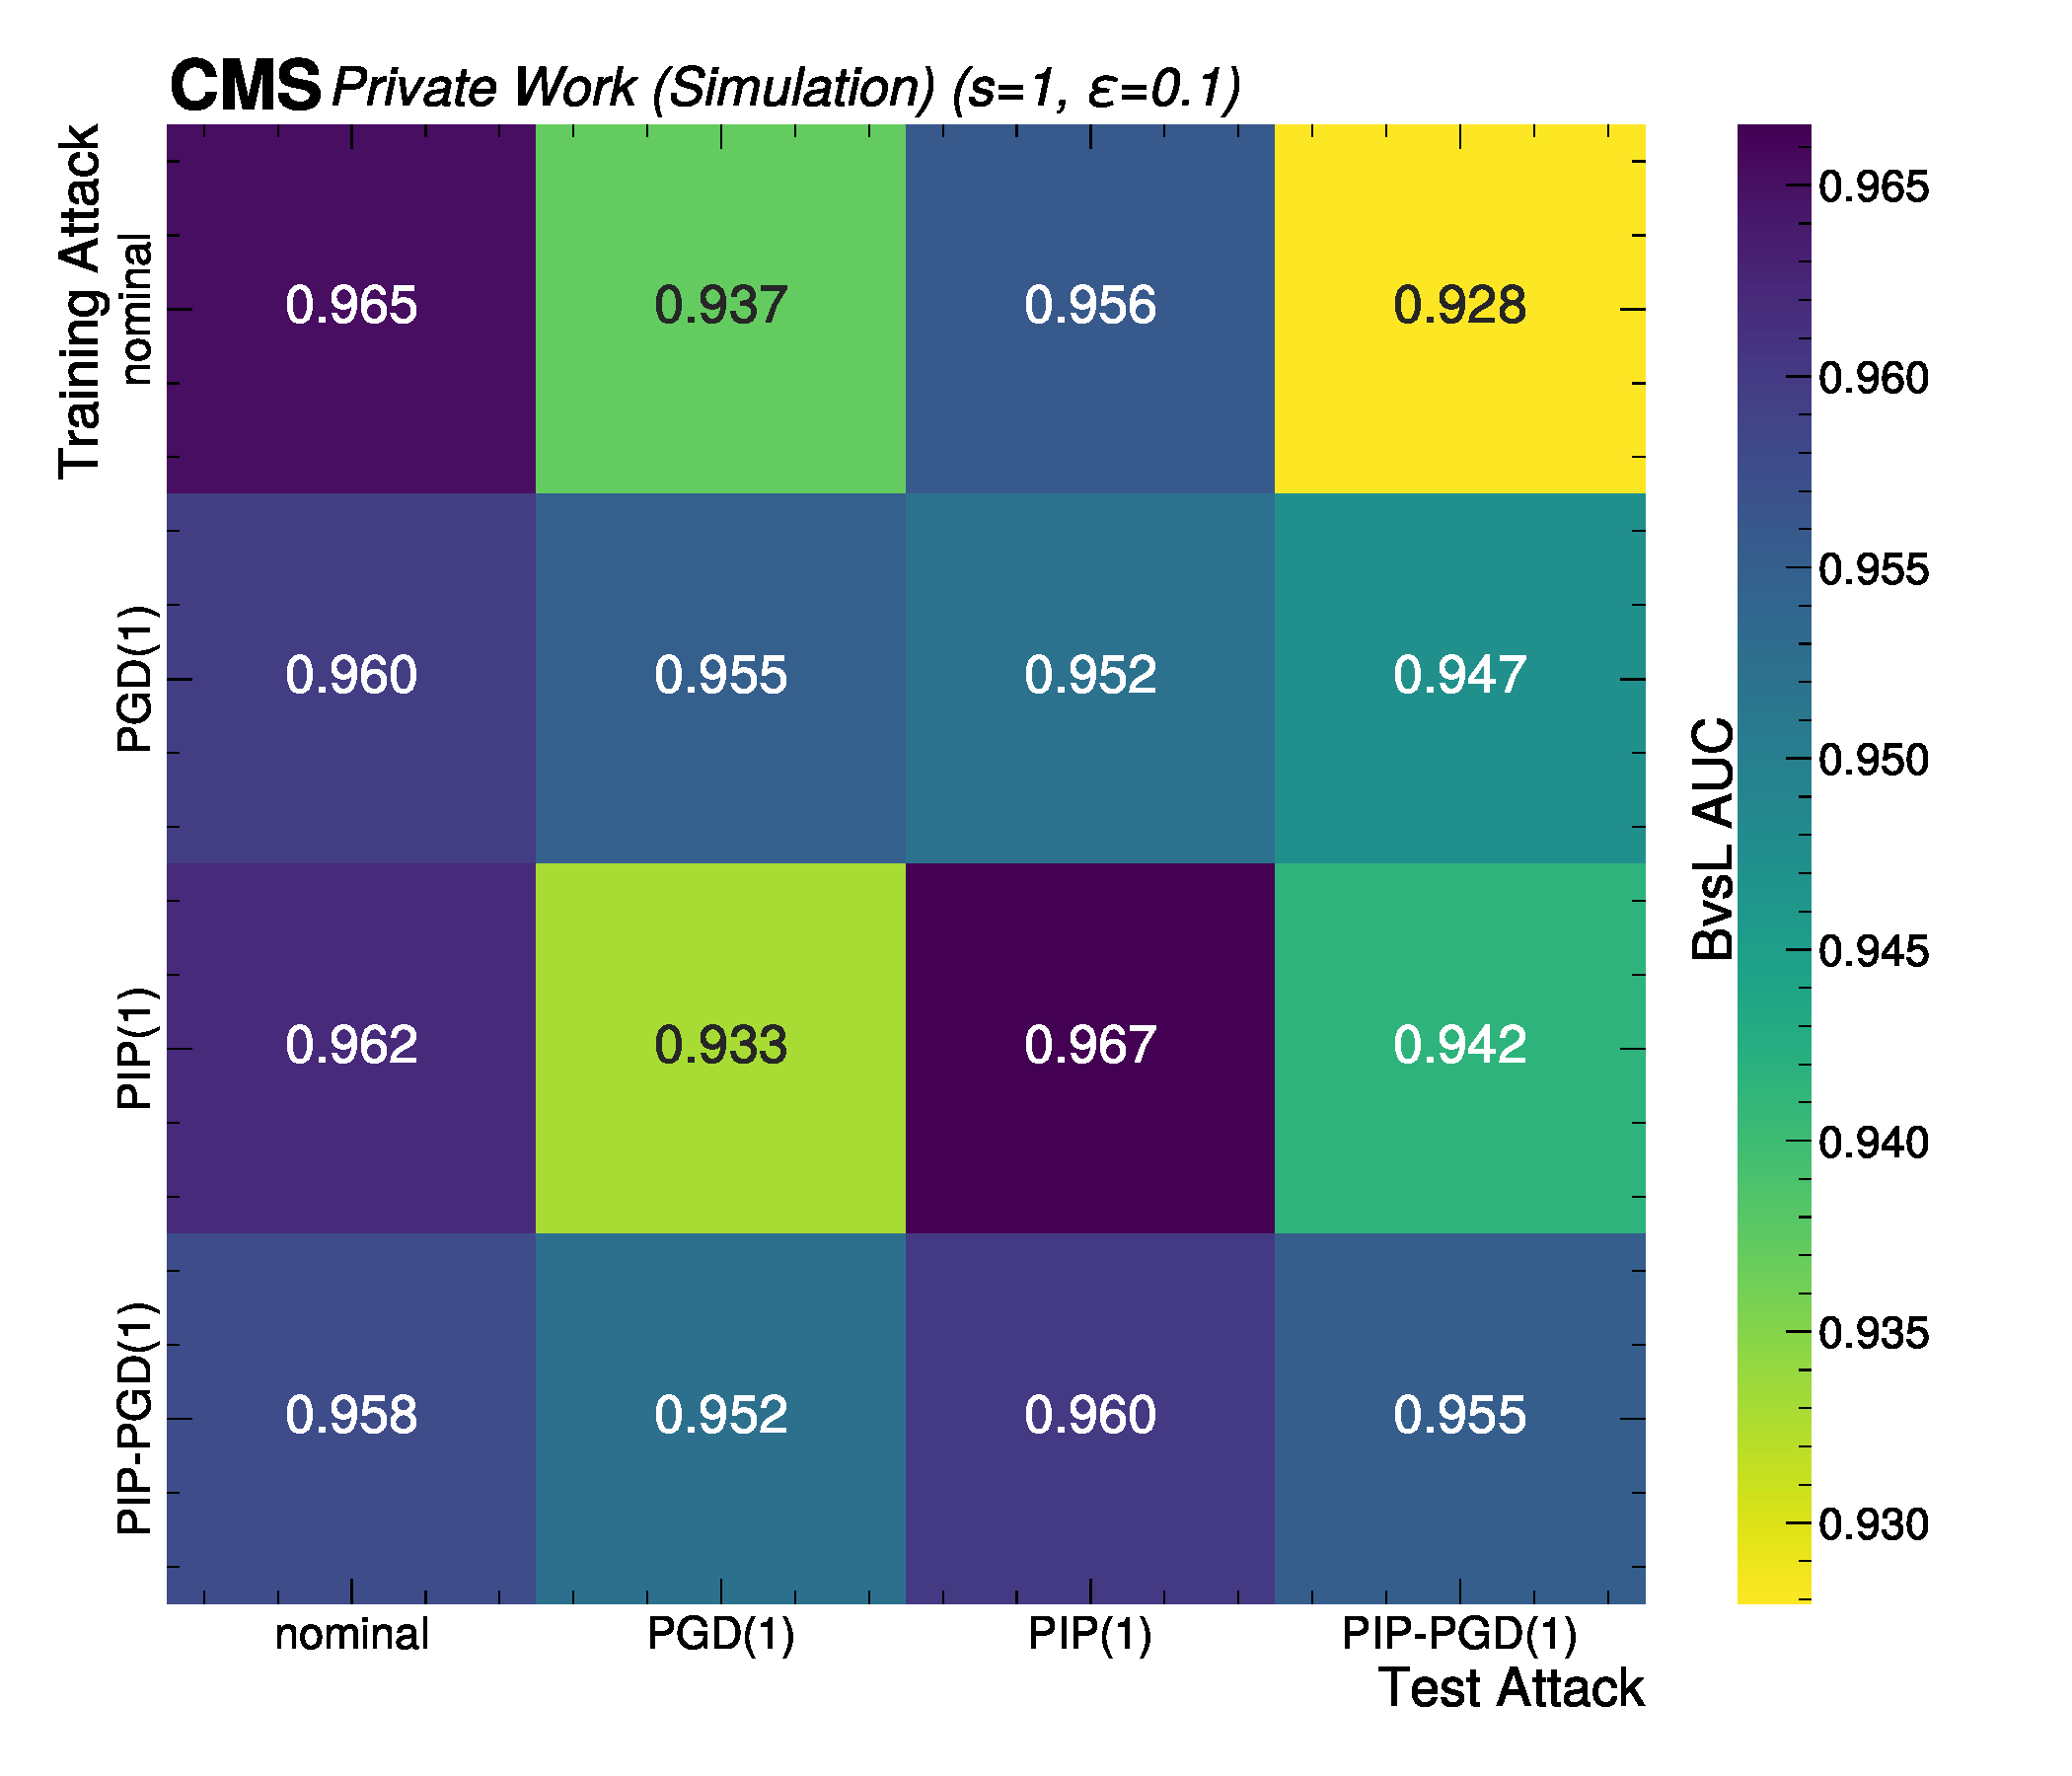
\includegraphics[width=15cm]{media/cross_robustness.pdf}
    \caption{AUC score for BvsL misidentification for all combinations of adversarial training and adversarial testing between nominal, PGD(1), PIP(1), and joint PIP-PGD(1) attacks with a sharpness of $s=1.0$ and $\epsilon=0.1$ while attributing for individual features.}
    \label{fig:cross_robustness}
\end{figure}

Figure \ref{fig:cross_robustness} illustrates a key property of adversarial training with integer-based attacks. The model trained on PIP achieves excellent performance against the same attack ($AUC = 0.967$), slightly outperforming the nominal model on unperturbed data ($AUC = 0.965$). This suggests strong adaptation to the characteristic perturbations of probabilistic integer modifications. However, this enhanced robustness is highly specific to the trained attack pattern. When evaluated against other attacks, such as PGD or PIP-PGD, performance degrades noticeably, indicating a form of adversarial overfitting where the model resists a narrow class of perturbations but struggles to generalize.

In contrast, adversarial training with the PIP-PGD strategy yields more balanced robustness across all tested attack scenarios. Although its AUC on the PIP attack is slightly lower than that of models trained solely on PIP or PGD, the combined model exhibits better transferability, maintaining robust performance under both PIP ($AUC = 0.960$) and PGD ($AUC = 0.952$) attacks. This suggests that combined adversarial training mitigates attack-specific overfitting, fostering a more generalizable defence.

Models trained solely on PGD struggle to achieve robustness against integer-based attacks, with an AUC of  $\le0.952$, though they remain stable against PGD perturbations.

Overall, the PIP-PGD training strategy offers the best cross-attack robustness while closely preserving nominal performance, with degradation of approximately 1.3\% for PGD-perturbed data, 0.5\% for PIP-perturbed data, and 1\% for PIP-PGD-perturbed data.